\documentclass[10pt,a4paper,twoside]{book}

\input{../../../Libri/template_dispense.tex}

	\usepackage{geometry}
	\geometry{
		nomarginpar, % Toglie doppi margini
		margin=1in, % Imposta i margini a 1 inch
	}

\usepackage{chngcntr}
\counterwithout{figure}{chapter}
\counterwithout{equation}{chapter}

\allowdisplaybreaks[4] % Consente di rompere equazioni su più pagine

%%%%%%%%%%%%%%%%%%%%%%%%%%%%%%%%%%%%%%%%%%%%%%%
%%%%%%%%%%%%%%%%%%%%%%%%%%%%%%%%%%%%%%%%%%%%%%%


\begin{document}

%%%%%%%%%%%%%%%%%%%%%%%%%%%%%%%%%%%%%%%%%%%%%%%
%%%%%%%%%%%%%%%%%%%%%%%%%%%%%%%%%%%%%%%%%%%%%%%

\frontmatter % The pages after this command and before the command \mainmatter, will be numbered with lowercase Roman numerals.

\pagestyle{empty} % SWITCHA PER NON AVERE NUMERO PAGINA
\vspace*{\fill}
%Teo Bucci \\
\begin{center}
	{\large \textsc{Appunti di}}\\
	\vspace*{0.4cm}
	{\Huge \textsc{Meccanica dei Continui}}\\
	\vspace*{1cm}
	{\large {Dalle lezioni del Prof. Maurizio Vianello}}\\
	\vspace*{0.1cm}
	{\large per il corso di Ingegneria Matematica}\\
	\vspace*{0.4cm}
	{\large {di Teo Bucci}}\\
	\vspace*{1cm}
	Politecnico di Milano\\
	A.A. 2020/2021
\end{center}
\vspace*{\fill}
\newpage

%%%%%%%%%%%%%%%%%%%%%%%%%%%%%%%%%%%%%%%%%%%%%%%
%%%%%%%%%%%%%%%%%%%%%%%%%%%%%%%%%%%%%%%%%%%%%%%

{\Large \textit{Appunti di Meccanica dei Continui}}

\vspace*{\fill}

\textbf{Disclaimer.}

In questo testo sono raccolti gli appunti tratti dalle lezioni del corso di Meccanica dei Continui, tenuto dal Professor Maurizio Vianello per il corso di Ingegneria Matematica, al Politecnico di Milano, nell'anno 2020/21.

La proprietà intellettuale rimane al docente sopracitato, il quale non ha revisionato la seguente opera, che si presenta unicamente come un supporto ulteriore alle lezioni, fatta da studenti per studenti, senza pretese di sostituire libri di testo ufficiali o la frequenza delle lezioni. La maggior parte delle illustrazioni è tratta dei disegni del docente, a lui rimane anche la proprietà intellettuale di esse.

%\textcopyright \ Gli autori, tutti i diritti riservati

Sono proibite tutte le riproduzioni senza autorizzazione scritta degli autori.

Revisione del \today

Developed by Teo Bucci - \texttt{teobucci8@gmail.com}\\ \\
Compiled with \ensuremath\heartsuit \\

%\textbf{Prefazione}

Per segnalare eventuali errori o suggerimenti potete contattare gli autori.

\newpage

%%%%%%%%%%%%%%%%%%%%%%%%%%%%%%%%%%%%%%%%%%%%%%%
%%%%%%%%%%%%%%%%%%%%%%%%%%%%%%%%%%%%%%%%%%%%%%%

% INDICE

\tableofcontents
\addtocontents{toc}{\protect\thispagestyle{empty}}
\thispagestyle{empty}
%\newpage

%%%%%%%%%%%%%%%%%%%%%%%%%%%%%%%%%%%%%%%%%%%%%%%
%%%%%%%%%%%%%%%%%%%%%%%%%%%%%%%%%%%%%%%%%%%%%%%

% PAGINA VUOTA PER FAR PARTIRE IL CAPITOLO IN UNA PAGINA DISPARI
%\myNewEmptyPage

\AtEndDocument{\cleardoublepage}

%%%%%%%%%%%%%%%%%%%%%%%%%%%%%%%%%%%%%%%%%%%%%%%
%%%%%%%%%%%%%%%%%%%%%%%%%%%%%%%%%%%%%%%%%%%%%%%

\mainmatter % This will restart the page counter and change the style to Arabic numbers

\pagestyle{fancy} % RISWITCHA PER RIAVERE IL NUMERO PAGINA
%\setcounter{page}{1} % FA RIPARTIRE IL CONTATORE PAGINA DA 1



%%%%%%%%%%%%%%%%%%%%%%%%%%%%%%%%%%%%%%%%%%%%%%%
%%%%%%%%%%%%%%%%%%%%%%%%%%%%%%%%%%%%%%%%%%%%%%%

\chapter{Corpi e deformazioni}

Studia i corpi deformabili. Abbiamo una \textbf{configurazione di riferimento}, poi il corpo viene collocato in un contesto e viene deformato in una \textbf{configurazione attuale}.

\fg[La deformazione e la sua inversa creano una corrispondenza biunivoca e regolare fra $\mathcal{B}_{\ast }$ e la configurazione deformata $\mathcal{B}$.]{0.4}{c0811ba9304bc37b90940e848c7072fb-MM3vWHMCKX}

I punti della configurazione di riferimento li indico con $p$ e con $x$ quelli della configurazione attuale. C'è una \textbf{deformazione}, cioè una corrispondenza
\begin{itemize}
\item uno a uno, 
\item regolare, almeno $C^{2}$
\end{itemize}
\begin{equation*}
\mathbf{f} :\mathcal{B}_{*}\rightarrow \mathcal{E}^{3} \ \ \ \ \mathbf{x} =\mathbf{f}(\mathbf{p} ,t)
\end{equation*}
Questa storia dell'uno a uno mi convince poco nel caso di autocontatto, quindi è uno a uno \textit{all'interno}.

\fg{0.2}{5c014c68cb931abd95bdd2a202257039-WIdel4Rb4w}

Questa storia del regolare mi convince poco nel caso di fratture

\fg{0.2}{dd7923f5e7224e013de65a4ca13c5730-srDfZzMMty}

Dicendo $\mathbf{x} =\mathbf{f}(\mathbf{p} ,t)$ stiamo dicendo che il punto materiale $\mathbf{p}$ al tempo $t$ va a collocarsi nel punto dello spazio $\mathbf{x}$. I punti materiali occupano punti dello spazio in funzione del tempo. Prendiamo un sistema di coordinate solidale all'osservatore, come assegnamo questa $\mathbf{f}$?
\begin{equation*}
\mathbf{p} =( X_{1} ,X_{2} ,X_{3}) \ \ \ \ \mathbf{x} =( x_{1} ,x_{2} ,x_{3})
\end{equation*}
Quindi la deformazione in realtà è
\begin{gather*}
x_{1} =f_{1}( X_{1} ,X_{2} ,X_{3} ,t)\\
x_{2} =f_{2}( X_{1} ,X_{2} ,X_{3} ,t)\\
x_{3} =f_{3}( X_{1} ,X_{2} ,X_{3} ,t)
\end{gather*}
A volte indicata anche con $\mathbf{x} =\mathbf{\chi }(\mathbf{p} ,t)$.
\section{Gradiente di deformazione}

Che relazione c'è tra le due frecce rosse?

\fg{0.4}{4d858e04c461555080cfb78fb5dfbbcb-kYmpfAANd1}

\begin{equation*}
\mathbf{f}(\mathbf{p} +\mathbf{h}) -\mathbf{f}(\mathbf{p}) =Df(\mathbf{p})[\mathbf{h}] +o(\mathbf{h})
\end{equation*}
Dove $Df$ è la trasformazione lineare che rende vera quell'uguaglianza. Questo $Df$ è chiamato \textbf{gradiente di deformazione}, che è un tensore.
\begin{equation*}
Df:\mathcal{V}\rightarrow \mathcal{V}
\end{equation*}
che chiamiamo $\mathbf{F}$
\begin{equation*}
\mathbf{F} :\mathcal{V}\rightarrow \mathcal{V}
\end{equation*}
Le sue componenti sono
\begin{equation*}
F_{ik} =\left[\frac{\partial f_{i}}{\partial x_{j}}\right]
\end{equation*}
Qui non c'è un campo, è un gradiente tra virgolette, matematicamente c'è un'analogia, ma non c'è un campo di cui fare il gradiente.

\fg{0.4}{9f68572fea8778d5ba527dd25be3d821-xRkRn0ND9m}

$\mathbf{p} +\mathbf{u}$ va a finire con buona approssimazione in $\mathbf{f}(\mathbf{p})$ più la trasformazione lineare $\mathbf{F}(\mathbf{u})$, questa cosa funziona meglio al tendere di $\mathbf{u}\rightarrow \mathbf{0}$.
\begin{equation*}
\mathbf{f}(\mathbf{p} +\mathbf{u}) =\mathbf{f}(\mathbf{p}) +\mathbf{Fu} +o(\mathbf{u})
\end{equation*}
che posso scrivere anche come
\begin{equation*}
\Delta \mathbf{x} =\mathbf{F} \Delta \mathbf{p} +o( \Delta \mathbf{p})
\end{equation*}
Posso scriverli anche in forma infinitesima
\begin{equation*}
\boxed{d\mathbf{x} =\mathbf{F} d\mathbf{p}}
\end{equation*}
che è un'uguaglianza esatta, cioè a meno di infinitesimi superiori.

Chiediamo a priori, per motivi successivi, che sia
\begin{equation*}
\mathrm{det}\mathbf{F}  >0
\end{equation*}
in aggiunta alle proprietà di regolarità e uno a uno della deformazione.

Consideriamo delle deformazioni particolarmente semplici.
\section{Deformazioni omogenee}

In queste deformazioni $\mathbf{F}$ è costante, non c'è l'o piccolo. Sono la prima approssimazione di una deformazione.
\begin{equation*}
\mathbf{f}(\mathbf{q}) =\mathbf{f}(\mathbf{p}) +\mathbf{F}(\mathbf{q} -\mathbf{p})\cancel{+o(\mathbf{q} -\mathbf{p})}
\end{equation*}
In questo mondo ci concentreremo sulle deformazioni che lasciano fisso un punto.
\section{Deformazioni omogenee con punto fisso}
\begin{equation*}
\begin{aligned}
\mathbf{f}(\mathbf{q}) & =\mathbf{\textcolor[rgb]{0.82,0.01,0.11}{f}}\textcolor[rgb]{0.82,0.01,0.11}{(}\textcolor[rgb]{0.82,0.01,0.11}{\overline{\mathbf{p}}}\textcolor[rgb]{0.82,0.01,0.11}{)} +\mathbf{F}(\mathbf{q} -\overline{\mathbf{p}})\\
 & =\textcolor[rgb]{0.82,0.01,0.11}{\overline{\mathbf{p}}} +\mathbf{F}(\mathbf{q} -\overline{\mathbf{p}})
\end{aligned}
\end{equation*}
Se conosco il punto fisso e il gradiente di deformazione, allora conosco la deformazione. Ogni deformazione omogenea è pari a una traslazione + una deformazione omogenea con punto fisso, perciò ci concentriamo su queste ultime, dato che le transazioni non cambiano la vera e propria deformazione.

Tutti i punti vicino a $\mathbf{p}$ sono approssimabili a una trasformazione omogenea, tutte le deformazioni sono localmente omogenee.
\section{Rotazioni}

Indichiamo l'insieme dei tensori ortogonali con
\begin{equation*}
\boxed{\mathbf{Q} \in \mathrm{Orth}} \ \ \Leftrightarrow \ \ \boxed{\mathbf{Q}^{T} =\mathbf{Q}^{-1}}
\end{equation*}
e sono tensori che preservano il prodotto scalare
\begin{equation*}
\mathbf{Qa} \cdotp \mathbf{Qb} =\mathbf{a} \cdotp \mathbf{b}
\end{equation*}
Tutti i tensori ortogonali hanno determinante $\pm 1$
\begin{equation*}
\mathrm{det}(\mathbf{I}) =\mathrm{det}(\mathbf{Q}) \cdotp \mathrm{det}\left(\mathbf{Q}^{T}\right) =[\mathrm{det}(\mathbf{Q})]^{2} \ \ \Rightarrow \ \ \mathrm{det}\mathbf{Q} =\pm 1
\end{equation*}
Diciamo che una \textbf{rotazione} è una trasformazione lineare su spazi vettoriali, un tensore
\begin{equation*}
\boxed{\mathbf{R} \in \mathrm{Rot}} \ \ \Leftrightarrow \ \ \boxed{\mathbf{R} \in \mathrm{Orth} ,\ \mathrm{det}\mathbf{R} =1}
\end{equation*}
Se $\mathbf{R}_{1} ,\mathbf{R}_{2}$ sono due rotazioni allora $\mathbf{R}_{1}\mathbf{R}_{2}$ ed $\mathbf{R}_{2}\mathbf{R}_{1}$ sono rotazioni composte.
\subsection{Teorema di esistenza dell'asse di rotazione}

\textit{Per ogni rotazione esiste un asse di rotazione.}

È quell'asse $\mathbf{e}$ tale che $\mathbf{Re} =\mathbf{e}$.

\textit{Dimostrazione.}

Infatti sapendo che $\mathbf{R}^{T}\mathbf{R} =\mathbf{I}$ e $\mathrm{det}\mathbf{R} =1$
\begin{equation*}
\begin{aligned}
\mathbf{R}^{T}(\mathbf{R} -\mathbf{I}) & =-(\mathbf{R} -\mathbf{I})^{T}\\
\mathbf{R}^{T}\mathbf{R} -\mathbf{R}^{T} & =-\mathbf{R}^{T} +\mathbf{I}\\
\mathbf{I} -\mathbf{R}^{T} & =-\mathbf{R}^{T} +\mathbf{I}
\end{aligned}
\end{equation*}
Allora
\begin{equation*}
\begin{aligned}
\mathrm{det}\left[\mathbf{R}^{T}(\mathbf{R} -\mathbf{I})\right] & =\mathrm{det}\left[ -(\mathbf{R} -\mathbf{I})^{T}\right]\\
\mathrm{det}\left(\mathbf{R}^{T}\right)\mathrm{det}(\mathbf{R} -\mathbf{I}) & =-\mathrm{det}(\mathbf{R} -\mathbf{I})\\
\mathrm{det}(\mathbf{R} -\mathbf{I}) & =-\mathrm{det}(\mathbf{R} -\mathbf{I})
\end{aligned}
\end{equation*}
Allora per forza
\begin{equation*}
\mathrm{det}(\mathbf{R} -\mathbf{I}) =0
\end{equation*}
Allora $\lambda =1$ è un autovalore di $\mathbf{R}$. Allora c'è un autovettore $\mathbf{v}$, e il suo corrispondente autoversore $\mathbf{e} =\frac{\mathbf{v}}{| \mathbf{v}| }$ tale che
\begin{equation*}
\mathbf{Re} =\lambda \mathbf{e} =\mathbf{e}
\end{equation*}
L'asse di rotazione è l'autospazio di $\lambda =1$.
\begin{oss}
Ricordiamo questo risultato di Algebra Lineare sul prodotto matrici vettori\footnote{ovvero possiamo spostare la matrice più a \textit{sinistra} dall'altra parte del prodotto scalare, sempre a \textit{sinistra}, facendone il trasposto.}
\begin{equation*}
\mathbf{ABc} \cdotp \mathbf{d} =\mathbf{Bc} \cdotp \mathbf{A}^{T}\mathbf{d} =\mathbf{c} \cdotp \mathbf{B}^{T}\mathbf{A}^{T}\mathbf{d}
\end{equation*}
I vettori perpendicolari all'asse di rotazione, rimangono perpendicolari
\begin{equation*}
\mathbf{a} \Bot \mathbf{e} \ \ \Rightarrow \ \ \mathbf{a\cdotp e} =0=\mathbf{Ia} \cdotp \mathbf{e} =\mathbf{R}^{T}\mathbf{Ra} \cdotp \mathbf{e} =\mathbf{Ra} \cdotp \mathbf{Re} =\mathbf{Ra} \cdotp \mathbf{e} \ \ \Rightarrow \ \ \mathbf{Ra} \Bot \mathbf{e}
\end{equation*}
Le rotazioni non alterano il modulo dei vettori
\begin{equation*}
| \mathbf{Ra}| ^{2} =\mathbf{Ra} \cdotp \mathbf{Ra} =\mathbf{R}^{T}\mathbf{Ra} \cdotp \mathbf{a} =\mathbf{a} \cdotp \mathbf{a} =| \mathbf{a}| ^{2}
\end{equation*}
\end{oss}
Definiamo un \textbf{tensore simmetrico}
\begin{equation*}
\boxed{\mathbf{S} \in \mathrm{Sym}} \ \ \Leftrightarrow \ \ \boxed{\mathbf{S} =\mathbf{S}^{T}}
\end{equation*}
Definiamo un \textbf{tensore simmetrico positivo}
\begin{equation*}
\boxed{\mathbf{S} \in \mathrm{Sym}^{+}} \ \ \Leftrightarrow \ \ \boxed{\mathbf{S} \in \mathrm{Sym} \ \land \ \mathbf{Sa} \cdotp \mathbf{a}  >0\ \ \forall \mathbf{a} \neq \mathbf{0}}
\end{equation*}
\subsection{Teorema della radice quadrata}

Sia $\mathbf{C} \in \mathrm{Sym}^{+}$ allora $\exists !\ \mathbf{U} \in \mathrm{Sym}^{+}$ tale che $\mathbf{U}^{2} =\mathbf{C}$, cioè $\mathbf{U} =\sqrt{\mathbf{C}}$.

\textit{Dimostrazione.}
\begin{itemize}
\item \textit{Esistenza.}

La matrice $\mathbf{C}$ essendo simmetrica e definita positiva si può diagonalizzare:

\begin{equation*}
\mathbf{C} =\begin{bmatrix}
\lambda ^{2}_{1} & 0 & 0\\
0 & \lambda ^{2}_{2} & 0\\
0 & 0 & \lambda ^{2}_{3}
\end{bmatrix}
\end{equation*}

rispetto a una terna. Rispetto alla stessa definisco:

\begin{equation*}
\mathbf{U} =\begin{bmatrix}
\lambda _{1} & 0 & 0\\
0 & \lambda _{2} & 0\\
0 & 0 & \lambda _{3}
\end{bmatrix}
\end{equation*}
\item \textit{Unicità.}

L'unicità è garantita dal positivo. Supponiamo ne esista un'altro, diverso, $\overline{\mathbf{U}}$.

\begin{equation*}
\mathbf{U}^{2} =\mathbf{C} \ \ \ \ \overline{\mathbf{U}}^{2} =\mathbf{C} \ \ \ \ \overline{\mathbf{U}} \neq \mathbf{U}
\end{equation*}

Prendiamo un autovalore e un autovettore di $\mathbf{U}$

\begin{equation*}
\mathbf{Ue} =\lambda \mathbf{e} \ \ \ \ \lambda  >0
\end{equation*}

allora

\begin{equation*}
\mathbf{U}^{2}\mathbf{e} =\mathbf{UUe} =\mathbf{U} \lambda \mathbf{e} =\lambda \mathbf{Ue} =\lambda ^{2}\mathbf{e} \ \ \Rightarrow \ \ \mathbf{Ce} =\lambda ^{2}\mathbf{e}
\end{equation*}

allora

\begin{equation*}
\begin{aligned}
(\overline{\mathbf{U}} +\lambda \mathbf{I})(\overline{\mathbf{U}} -\lambda \mathbf{I})\mathbf{e} & =\left(\overline{\mathbf{U}}^{2} +\lambda \overline{\mathbf{U}} -\lambda \overline{\mathbf{U}} -\lambda ^{2}\mathbf{I}\right)\mathbf{e}\\
 & =\left(\mathbf{C} -\lambda ^{2}\mathbf{I}\right)\mathbf{e}\\
 & =\mathbf{Ce} -\lambda ^{2}\mathbf{e} =\mathbf{0}
\end{aligned}
\end{equation*}

scriviamo questa uguaglianza come

\begin{equation*}
(\overline{\mathbf{U}} +\lambda \mathbf{I})\underbrace{(\overline{\mathbf{U}} -\lambda \mathbf{I})\mathbf{e}}_{\mathbf{w}} =(\overline{\mathbf{U}} +\lambda \mathbf{I})\mathbf{w} =\mathbf{0} \ \ \Rightarrow \ \ \overline{\mathbf{U}}\mathbf{w} =-\lambda \mathbf{w}
\end{equation*}

ho due possibilità: $\mathbf{w} =\mathbf{0} ,\mathbf{w} \neq \mathbf{0}$.
\begin{itemize}
\item Se $\mathbf{w} \neq \mathbf{0}$ allora $\mathbf{w}$ sarebbe autovettore di $\overline{\mathbf{U}}$ con autovalore $-\lambda $. Ciò è impossibile perché $\overline{\mathbf{U}}$ avrebbe un autovalore negativo, mentre invece è un tensore simmetrico positivo.
\item Quindi $\mathbf{w} =\mathbf{0}$\begin{equation*}
\mathbf{w} =(\overline{\mathbf{U}} -\lambda \mathbf{I})\mathbf{e} =0\ \ \Rightarrow \ \ \overline{\mathbf{U}}\mathbf{e} =\lambda \mathbf{e}
\end{equation*}
\end{itemize}

ovvero ogni autovalore e autovettore di $\mathbf{U}$ sono autovalori e autovettori di $\overline{\mathbf{U}}$ e viceversa. Quindi hanno i medesimi autovalori e autovettori: dall'algebra, $\mathbf{U} =\overline{\mathbf{U}}$.
\end{itemize}
\subsection{Teorema di decomposizione polare}

Sia $\mathbf{F} \in \mathrm{Lin}^{+}$\footnote{Tensori a determinante positivo, come il gradiente di deformazione.}, allora $\exists !\ \mathbf{R} ,\mathbf{U} ,\mathbf{V}$, di cui $\mathbf{R} \in \mathrm{Rot}$ e $\mathbf{U} ,\mathbf{V} \in \mathrm{Sym}^{+}$ tali che
\begin{equation*}
\boxed{\mathbf{F} =\mathbf{RU} =\mathbf{VR}}
\end{equation*}
\textit{Dimostrazione.}

Il tensore che definiamo
\begin{equation*}
\boxed{\mathbf{C} =\mathbf{F}^{T}\mathbf{F}}
\end{equation*}
è simmetrico:
\begin{equation*}
\mathbf{C}^{T} =\left(\mathbf{F}^{T}\mathbf{F}\right)^{T} =\mathbf{F}^{T}\left(\mathbf{F}^{T}\right)^{T} =\mathbf{F}^{T}\mathbf{F} =\mathbf{C}
\end{equation*}
e definito positivo (ricordiamo che $\mathbf{F}$ è invertibile e $\mathbf{Fa} =\mathbf{0}$ solo se $\mathbf{a} =\mathbf{0}$):
\begin{equation*}
\mathbf{Ca} \cdotp \mathbf{a} =\mathbf{F}^{T}\mathbf{Fa} \cdotp \mathbf{a} =\mathbf{Fa} \cdotp \mathbf{Fa} =| \mathbf{Fa}| ^{2}  >0\ \ \forall \mathbf{a} \neq \mathbf{0}
\end{equation*}
Quindi abbiamo $\mathbf{C} \in \mathrm{Sym}^{+}$, allora per il teorema della radice quadrata
\begin{equation*}
\exists !\ \mathbf{U} \in \mathrm{Sym}^{+} \ \text{tale che} \ \boxed{\mathbf{U} =\sqrt{\mathbf{C}} =\sqrt{\mathbf{F}^{T}\mathbf{F}}}
\end{equation*}
Abbiamo quindi determinato $\mathbf{C}$ ed $\mathbf{U}$, per avere l'uguaglianza $\mathbf{F} =\mathbf{RU}$ ci serve da determinare come è fatto $\mathbf{R}$, la sua unicità e il fatto che sia una rotazione.
\begin{equation*}
\boxed{\mathbf{R} =\mathbf{FU}^{-1}}
\end{equation*}
Verifichiamo che sia una rotazione:
\begin{itemize}
\item è ortogonale\begin{align*}
\mathbf{R}^{T}\mathbf{R} & =\left(\mathbf{FU}^{-1}\right)^{T}\left(\mathbf{FU}^{-1}\right) =\mathbf{U}^{-T}\mathbf{F}^{T}\mathbf{FU}^{-1}\\
 & =\mathbf{U}^{-1}\mathbf{U}^{2}\mathbf{U}^{-1} =\mathbf{U}^{-1}\mathbf{UUU}^{-1} =\mathbf{II} =\mathbf{I}
\end{align*}
\item essendo ortogonale il suo determinante può essere solo $\pm 1$\begin{equation*}
\mathrm{det}\mathbf{R} =(\mathrm{det}\mathbf{F})\left(\mathrm{det}\mathbf{U}^{-1}\right) =\frac{\mathrm{det}\mathbf{F}}{\mathrm{det}\mathbf{U}}
\end{equation*}

ma il determinante di $\mathbf{F}$ è positivo per ipotesi e il determinante di $\mathbf{U}$ è positivo essendo simmetrico e definito positivo, quindi per forza $\mathrm{det}\mathbf{R} =1$.
\end{itemize}

Quindi $\mathbf{R}$ definita come sopra, è una rotazione, ed è unica per costruzione.

Passiamo alla seconda parte del teorema, per determinare $\mathbf{V}$ è sufficiente definirlo come
\begin{equation*}
\boxed{\mathbf{V} =\mathbf{RUR}^{T}}
\end{equation*}
e far vedere che è $\mathrm{Sym}^{+}$.
\begin{itemize}
\item È simmetrico, grazie alla simmetria di $\mathbf{U}$

\begin{equation*}
\mathbf{V}^{T} =\left(\mathbf{RUR}^{T}\right)^{T} =\mathbf{RU}^{T}\mathbf{R}^{T} =\mathbf{RUR}^{T} =\mathbf{V}
\end{equation*}
\item È positivo, grazie alla positività di $\mathbf{U}$ e al fatto che $\mathrm{det}\mathbf{R} \neq 0$

\begin{equation*}
\mathbf{Va} \cdot \mathbf{a} =\mathbf{RUR}^{T}\mathbf{a} \cdot \mathbf{a} =\mathbf{U}\left(\mathbf{R}^{T}\mathbf{a}\right) \cdot \left(\mathbf{R}^{T}\mathbf{a}\right)  >0\ \ \text{per ogni} \ \mathbf{a} \neq \mathbf{0}
\end{equation*}
\end{itemize}
\begin{oss}
Essendo $\mathbf{V} =\mathbf{RUR}^{T}$, prendiamo $\lambda ,\mathbf{e}$ tali che
\begin{equation*}
\mathbf{Ue} =\lambda \mathbf{e} \ \ \lambda  >0
\end{equation*}
se faccio
\begin{equation*}
\mathbf{V}(\mathbf{Re}) =\mathbf{RUR}^{T}(\mathbf{Re}) =\mathbf{RUe} =\mathbf{R}( \lambda \mathbf{e}) =\lambda (\mathbf{Re})
\end{equation*}
quind $\lambda $ e $\mathbf{Re}$ sono autovalori e autovettori di $\mathbf{V}$, ovvero $\mathbf{U}$ e $\mathbf{V}$ \emph{hanno gli stessi autovalori, mentre gli autovettori / autospazi si ottengono per rotazione tramite} $\mathbf{R}$. Inoltre vale
\begin{equation*}
\mathbf{RU} =\mathbf{VR} \ \ \Rightarrow \ \ \mathbf{U} =\mathbf{R}^{T}\mathbf{VR}
\end{equation*}
\end{oss}
\section{Deformazioni pure}

Consideriamo $\mathbf{U} \in \mathrm{Sym}^{+}$. Supponiamo che $\mathbf{e}_{i}$ sia una terna ortonormale di autovettori di $\mathbf{U}$. Ricordiamo che la matrice del prodotto tensore è fatta così
\begin{equation*}
[\mathbf{a} \otimes \mathbf{b}] =\begin{bmatrix}
a_{1} b_{1} & a_{1} b_{2} & a_{1} b_{3}\\
a_{2} b_{1} & a_{2} b_{2} & a_{2} b_{3}\\
a_{3} b_{1} & a_{3} b_{2} & a_{3} b_{3}
\end{bmatrix}
\end{equation*}
In questo sistema di riferimento calcoliamo i prodotti tensori degli $\mathbf{e}_{i}$
\begin{equation*}
\mathbf{e}_{1} \otimes \mathbf{e}_{1} =\begin{bmatrix}
1\cdotp 1 & 0 & 0\\
0 & 0 & 0\\
0 & 0 & 0
\end{bmatrix} =\begin{bmatrix}
1 & 0 & 0\\
0 & 0 & 0\\
0 & 0 & 0
\end{bmatrix}
\end{equation*}
e analogamente
\begin{equation*}
\mathbf{e}_{1} \otimes \mathbf{e}_{2} =\begin{bmatrix}
0 & 1 & 0\\
0 & 0 & 0\\
0 & 0 & 0
\end{bmatrix} \ \ \ \ \mathbf{e}_{2} \otimes \mathbf{e}_{3} =\begin{bmatrix}
0 & 0 & 0\\
0 & 0 & 1\\
0 & 0 & 0
\end{bmatrix}
\end{equation*}
Usando la terna di riferimento, la matrice del tensore $\mathbf{U}$ si può scrivere come
\begin{equation*}
\mathbf{U} =\begin{bmatrix}
\lambda _{1} & 0 & 0\\
0 & \lambda _{2} & 0\\
0 & 0 & \lambda _{3}
\end{bmatrix} =\lambda _{1}\begin{bmatrix}
1 & 0 & 0\\
0 & 0 & 0\\
0 & 0 & 0
\end{bmatrix} +\lambda _{2}\begin{bmatrix}
0 & 0 & 0\\
0 & 1 & 0\\
0 & 0 & 0
\end{bmatrix} +\lambda _{3}\begin{bmatrix}
0 & 0 & 0\\
0 & 0 & 0\\
0 & 0 & 1
\end{bmatrix}
\end{equation*}
ovvero
\begin{equation*}
\mathbf{U} =\lambda _{1}[\mathbf{e}_{1} \otimes \mathbf{e}_{1}] +\lambda _{2}[\mathbf{e}_{2} \otimes \mathbf{e}_{2}] +\lambda _{3}[\mathbf{e}_{3} \otimes \mathbf{e}_{3}] =\sum\limits ^{3}_{i=1} \lambda _{i}[\mathbf{e}_{i} \otimes \mathbf{e}_{i}]
\end{equation*}
Torniamo alle deformazioni omogenee con $\overline{\mathbf{p}}$ fisso e consideriamo due trasformazioni diverse
\begin{gather*}
\mathbf{f}_{1}(\mathbf{q}) =\overline{\mathbf{p}} +\mathbf{F}_{1}(\mathbf{q} -\overline{\mathbf{p}})\\
\mathbf{f}_{2}(\mathbf{q}) =\overline{\mathbf{p}} +\mathbf{F}_{2}(\mathbf{q} -\overline{\mathbf{p}})
\end{gather*}
cosa succede se faccio la composta?
\begin{equation*}
\begin{aligned}
(\mathbf{f}_{2} \circ \mathbf{f}_{1})(\mathbf{q}) =\mathbf{f}_{2}(\mathbf{f}_{1}(\mathbf{q})) & =\mathbf{f}_{2}(\overline{\mathbf{p}} +\mathbf{F}_{1}(\mathbf{q} -\overline{\mathbf{p}}))\\
 & =\overline{\mathbf{p}} +\mathbf{F}_{2}(\overline{\mathbf{p}} +\mathbf{F}_{1}(\mathbf{q} -\overline{\mathbf{p}}) -\overline{\mathbf{p}})\\
 & =\overline{\mathbf{p}} +\mathbf{F}_{2}(\mathbf{F}_{1}(\mathbf{q} -\overline{\mathbf{p}}))\\
 & =\overline{\mathbf{p}} +\mathbf{F}_{2}\mathbf{F}_{1}(\mathbf{q} -\overline{\mathbf{p}})
\end{aligned}
\end{equation*}
Leggiamo questa cosa nell'ottica della decomposizione polare
\begin{equation*}
\mathbf{f}(\mathbf{q}) =\overline{\mathbf{p}} +\mathbf{F}(\mathbf{q} -\overline{\mathbf{p}}) =\overline{\mathbf{p}} +\mathbf{RU}(\mathbf{q} -\overline{\mathbf{p}})
\end{equation*}
Quella $\mathbf{R}$ dà una rotazione, ma in che senso? Le rotazioni ruotano i \textit{vettori}, qui siamo nello spazio e stiamo parlando di \textit{punti}.
\begin{equation*}
\mathbf{r}(\mathbf{q}) =\overline{\mathbf{p}} +\mathbf{R}(\mathbf{q} -\overline{\mathbf{p}}) \ \ \Leftrightarrow \ \ \mathbf{r}(\mathbf{q}) -\overline{\mathbf{p}} =\mathbf{R}(\mathbf{q} -\overline{\mathbf{p}})
\end{equation*}
Stiamo ruotando il vettore $\mathbf{q} -\overline{\mathbf{p}}$ \textit{attorno} a $\overline{\mathbf{p}}$. Ricordando
\begin{equation*}
\mathbf{F} =\mathbf{RU} =\mathbf{VR}
\end{equation*}
e avendo capito che la $\mathbf{R}$ è una rotazione, deduciamo che $\mathbf{U}$ e $\mathbf{V}$ sono \textbf{deformazioni pure}. Per capirlo introduciamo una terna di riferimento e studiamo
\begin{equation*}
\mathbf{f}(\mathbf{q}) =\overline{\mathbf{p}} +\mathbf{U}(\mathbf{q} -\overline{\mathbf{p}})
\end{equation*}
mettiamo il punto fisso nell'origine
\begin{equation*}
\overline{\mathbf{p}} =( 0,0,0) \ \ \ \ \mathbf{q} =( X_{1} ,X_{2} ,X_{3}) \ \ \ \ \mathbf{f}(\mathbf{q}) =( x_{1} ,x_{2} ,x_{3})
\end{equation*}
Come assi prendo gli autovettori di $\mathbf{U}$ e ricordiamo che
\begin{equation*}
\mathbf{U} =\sum\limits ^{3}_{i=1} \lambda _{i}[\mathbf{e}_{i} \otimes \mathbf{e}_{i}]
\end{equation*}
allora
\begin{equation*}
\mathbf{f}(\mathbf{q}) =\overline{\mathbf{p}} +\left(\sum\limits ^{3}_{i=1} \lambda _{i}[\mathbf{e}_{i} \otimes \mathbf{e}_{i}]\right)(\mathbf{q} -\overline{\mathbf{p}}) =\left(\sum\limits ^{3}_{i=1} \lambda _{i}[\mathbf{e}_{i} \otimes \mathbf{e}_{i}]\right)(\mathbf{q})
\end{equation*}
cioé
\begin{equation*}
\mathbf{f}(\mathbf{q}) =( \lambda _{1}[\mathbf{e}_{1} \otimes \mathbf{e}_{1}] +\lambda _{2}[\mathbf{e}_{2} \otimes \mathbf{e}_{2}] +\lambda _{3}[\mathbf{e}_{3} \otimes \mathbf{e}_{3}])\underbrace{( X_{1}\mathbf{e}_{1} +X_{2}\mathbf{e}_{2} +X_{3}\mathbf{e}_{3})}_{(\mathbf{q})}
\end{equation*}
Per farlo ricordiamoci che
\begin{equation*}
(\mathbf{a} \otimes \mathbf{b})\mathbf{v} =(\mathbf{b} \cdotp \mathbf{v})\mathbf{a} \ \ \ \ \land \ \ \ \ \mathbf{e}_{i} \cdotp \mathbf{e}_{j} =0\ \forall i\neq j
\end{equation*}
Allora
\begin{equation*}
\boxed{\mathbf{f}(\mathbf{q}) =\lambda _{1} X_{1}\mathbf{e}_{1} +\lambda _{2} X_{2}\mathbf{e}_{2} +\lambda _{3} X_{3}\mathbf{e}_{3}}
\end{equation*}
cioé
\begin{equation*}
\begin{cases}
x_{1} =\lambda _{1} X_{1}\\
x_{2} =\lambda _{2} X_{2}\\
x_{3} =\lambda _{3} X_{3}
\end{cases}
\end{equation*}
quindi per passare dalle coordinate di $\overline{\mathbf{p}}$ a quelle di $\mathbf{q}$ stiamo facendo \textbf{un'estensione (o contrazione) lungo gli assi coordinati scegli come autovettori} di $\mathbf{U}$. Quindi possiamo avere deformazione pura seguita da rotazione, o viceversa. La rotazione è sempre la stessa, ma la deformazione è diversa (ruotata).
\subsection{Riassunto}
\begin{itemize}
\item Ogni deformazione finita è localmente omogenea
\item Ogni deformazione omogenea è a meno di una traslazione una deformazione omogenea con punto fisso
\item Ogni deformazione omogenea con punto fisso è la composizione di una rotazione preceduta (o seguita) da una deformazione pura
\item Ogni deformazione pura è l'insieme di $3$ estensioni (o contrazioni) lungo tre assi ortogonali, gli autospazi di $\mathbf{U}$, o $\mathbf{V}$.
\end{itemize}

\fg[Un cubo soggetto a una deformazione omogenea di gradiente $\mathbf{F}$. È possibile eseguire prima una deformazione pura $\mathbf{U}$ seguita da una rotazione $\mathbf{R}$ oppure la medesima rotazione $\mathbf{R}$ seguita da una deformazione pura $\mathbf{V}$: $\mathbf{F} =\mathbf{RU} =\mathbf{VR}$. Le deformazioni $\mathbf{U}$ e $\mathbf{V}$ avvengono secondo assi principali legati dalla rotazione $\mathbf{R}$ stessa.]{0.4}{4f3970c68ba5a6be4ef9d856bc106124-fPZOYGXnp2}

\section{Tensori di Cauchy-Green}

Avevamo già definito un certo tensore $\mathbf{C}$, che affianchiamo a $\mathbf{B}$
\begin{equation*}
\boxed{\mathbf{B} =\mathbf{FF}^{T}} \ \ \ \ \boxed{\mathbf{C} =\mathbf{F}^{T}\mathbf{F}}
\end{equation*}
chiaramente $\mathbf{B} ,\mathbf{C} \in \mathrm{Sym}^{+}$ per il teorema di decomposizione polare e si chiamano\footnote{per dove va a finire $\mathbf{F}$.}
\begin{itemize}
\item $\mathbf{B} =\mathbf{FF}^{T}$: \textbf{tensore di Cauchy-Green sinistro}
\item $\mathbf{C} =\mathbf{F}^{T}\mathbf{F}$: \textbf{tensore di Cauchy-Green destro}
\end{itemize}

Si ha che
\begin{equation*}
\boxed{\mathbf{B} =\mathbf{FF^{T}} =\mathbf{V}^{2}} \ \ \ \ \boxed{\mathbf{C} =\mathbf{F^{T} F} =\mathbf{U}^{2}}
\end{equation*}
\section{Stiramenti e deformazioni longitudinali}

Introduciamo una curva $\hat{\mathbf{p}}$ che passa per la configurazione di riferimento

\fg{0.4}{553bb69ce14330205436896ea3ff416a-1DTWFGH9He}

che ha $\mathbf{d}$ come versore tangente, detta $S$ l'ascissa curvilinea della configurazione di riferimento
\begin{equation*}
\frac{d\hat{\mathbf{p}}}{dS} =\mathbf{d}
\end{equation*}
Tramite $\mathbf{f}$ diventa una curva nella configurazione attuale
\begin{equation*}
\hat{\mathbf{x}}( S) =\mathbf{f}(\hat{\mathbf{p}}( S))
\end{equation*}
Derivo rispetto a $S$
\begin{equation*}
\frac{d\hat{\mathbf{x}}}{dS} =\frac{d\hat{\mathbf{x}}}{d\hat{\mathbf{p}}}\frac{d\hat{\mathbf{p}}}{dS} =\mathbf{Fd}
\end{equation*}
Derivo rispetto a $s$, l'ascissa curvilinea della configurazione attuale
\begin{equation*}
\frac{d\hat{\mathbf{x}}}{ds} =\mathbf{e}
\end{equation*}
Sostituendo nella relazione precedente
\begin{equation*}
\mathbf{Fd} =\frac{d\hat{\mathbf{x}}}{dS} =\frac{d\hat{\mathbf{x}}}{ds}\frac{ds}{dS} =\mathbf{e}\frac{ds}{dS} =\mathbf{e} \delta 
\end{equation*}
L'ultima quantità si chiama \textbf{coefficiente di stiramento}
\begin{equation*}
\boxed{\delta (\mathbf{d}) =\frac{ds}{dS}  >0} \ \ \ \ \boxed{\mathbf{Fd} =\mathbf{e} \delta }
\end{equation*}
che dipende dal punto e dalla curva scelta, dalla direzione.

Se $\delta (\mathbf{d})  >1$ localmente c'è allungamento, se $\delta (\mathbf{d}) < 1$ localmente c'è accorciamento.

Per calcolare in modo facile $\delta (\mathbf{d})$, sappiamo che $\mathbf{e} \cdotp \mathbf{e} =1$:
\begin{equation*}
\begin{aligned}
\mathbf{Fd} \cdotp \mathbf{Fd} & =\delta ^{2}(\mathbf{d})\\
\mathbf{F}^{T}\mathbf{Fd} \cdotp \mathbf{d} & =\delta ^{2}(\mathbf{d})\\
\mathbf{Cd} \cdotp \mathbf{d} & =\delta ^{2}(\mathbf{d})
\end{aligned}
\end{equation*}
allora essendo $\mathbf{C} \in \mathrm{Sym}^{+}$
\begin{equation*}
\boxed{\delta (\mathbf{d}) =\sqrt{\mathbf{Cd} \cdotp \mathbf{d}}}
\end{equation*}
Aggiungiamo il concetto di \textbf{deformazione longitudinale}
\begin{equation*}
\boxed{\varepsilon (\mathbf{d}) =\delta (\mathbf{d}) -1}
\end{equation*}
ha il significato di variazione di lunghezza per unità di lunghezza
\begin{equation*}
\varepsilon (\mathbf{d}) =\frac{ds}{dS} -1=\frac{ds-dS}{dS}
\end{equation*}
\section{Angoli di scorrimento}

Procedendo in modo simile deduciamo anche gli \textbf{angoli di scorrimento}.

\fg[Due filamenti si intersecano nella configurazione di riferimento secondo le direzioni dei versori ortogonali $\mathbf{d}_{1}$ e $\mathbf{d}_{2}$. Nella configurazione deformata le curve formano un angolo $\vartheta $, con angolo di scorrimento pari a $\gamma =\pi /2-\vartheta $.]{0.4}{31f0fdad07d10e67c64d57b9e78ebe4a-nXjNx2ku96}

Applichiamo la formula per lo stiramento a due direzioni diverse, prendendo $\mathbf{d}_{1}$ e $\mathbf{d}_{2}$ ortogonali
\begin{gather*}
\mathbf{Fd}_{1} =\delta (\mathbf{d}_{1})\mathbf{e}_{1}\\
\mathbf{Fd}_{2} =\delta (\mathbf{d}_{2})\mathbf{e}_{2}
\end{gather*}
Facciamone il prodotto scalare
\begin{equation*}
\begin{aligned}
\mathbf{Fd}_{1} \cdotp \mathbf{Fd}_{2} & =\delta (\mathbf{d}_{1})\mathbf{e}_{1} \cdotp \delta (\mathbf{d}_{2})\mathbf{e}_{2}\\
\mathbf{F}^{T}\mathbf{Fd}_{1} \cdotp \mathbf{d}_{2} & =\delta (\mathbf{d}_{1}) \delta (\mathbf{d}_{2})\mathbf{e}_{1} \cdotp \mathbf{e}_{2}\\
\mathbf{Cd}_{1} \cdotp \mathbf{d}_{2} & =\delta (\mathbf{d}_{1}) \delta (\mathbf{d}_{2})\cos \vartheta 
\end{aligned}
\end{equation*}
allora
\begin{equation*}
\boxed{\cos \vartheta =\frac{\mathbf{Cd}_{1} \cdotp \mathbf{d}_{2}}{\delta (\mathbf{d}_{1}) \delta (\mathbf{d}_{2})} =\frac{\mathbf{Cd}_{1} \cdotp \mathbf{d}_{2}}{\sqrt{\mathbf{Cd}_{1} \cdotp \mathbf{d}_{1}}\sqrt{\mathbf{Cd}_{2} \cdotp \mathbf{d}_{2}}}}
\end{equation*}
\begin{oss}
$\mathbf{C}$ ha degli autoversori, scopriamo subito che se chiamiamo tale terna $\mathbf{h}_{j}$ allora $\mathbf{Ch}_{i} \cdotp \mathbf{h}_{j} =0\ \forall i\neq j$, quindi $\cos \vartheta =0$, cioè se come direzioni prendiamo quelle degli autospazi, le direzioni saranno magari ruotate, ma \textit{ancora ortogonali}. Le direzioni degli autospazi di $\mathbf{C}$ si chiamano \textbf{direzioni principali di deformazione.}
\end{oss}
Definiamo inoltre
\begin{equation*}
\boxed{\gamma =\frac{\pi }{2} -\vartheta } \ \ \Rightarrow \ \ \sin \gamma =\frac{\mathbf{Cd}_{1} \cdotp \mathbf{d}_{2}}{\sqrt{\mathbf{Cd}_{1} \cdotp \mathbf{d}_{1}}\sqrt{\mathbf{Cd}_{2} \cdotp \mathbf{d}_{2}}}
\end{equation*}
che viene chiamato \textbf{angolo di scorrimento}. Lo scorrimento è nullo se $\vartheta =\pi /2$, se le curve si sono matenute ortogonali. Ci dice quanto si scostano dall'ortogonalità due curve.
\begin{itemize}
\item se $\gamma  >0$ l'angolo $\vartheta $ si stringe
\item se $\gamma < 0$ l'angolo $\vartheta $ si apre
\end{itemize}



Possiamo determinare le varie componenti della matrice tramite la relazione
\begin{equation*}
C_{ij} =\mathbf{Ce}_{i} \cdotp \mathbf{e}_{j}
\end{equation*}
Le componenti sulla diagonale sono pertanto gli \textbf{stiramenti principali}
\begin{gather*}
C_{11} =\mathbf{Ce}_{1} \cdotp \mathbf{e}_{1} =\delta ^{2}(\mathbf{e}_{1}) =\delta ^{2}_{1}\\
C_{22} =\mathbf{Ce}_{2} \cdotp \mathbf{e}_{2} =\delta ^{2}(\mathbf{e}_{2}) =\delta ^{2}_{2}\\
C_{33} =\mathbf{Ce}_{3} \cdotp \mathbf{e}_{3} =\delta ^{2}(\mathbf{e}_{3}) =\delta ^{2}_{3}
\end{gather*}
Le componenti fuori diagonale
\begin{equation*}
\cos \vartheta _{12} =\frac{\mathbf{Cd}_{1} \cdotp \mathbf{d}_{2}}{\sqrt{\mathbf{Cd}_{1} \cdotp \mathbf{d}_{1}}\sqrt{\mathbf{Cd}_{2} \cdotp \mathbf{d}_{2}}} =\frac{C_{12}}{\delta _{1} \delta _{2}} \ \ \Rightarrow \ \ C_{12} =\delta _{1} \delta _{2}\cos \vartheta _{12}
\end{equation*}
possiamo quindi costruire tutto il tensore $\mathbf{C}$
\begin{equation*}
\mathbf{C} =[ \delta _{i} \delta _{j}\cos \vartheta _{ij}] =\begin{bmatrix}
\delta ^{2}_{1} & \delta _{1} \delta _{2}\cos \vartheta _{12} & \delta _{1} \delta _{3}\cos \vartheta _{13}\\
\delta _{1} \delta _{2}\cos \vartheta _{12} & \delta ^{2}_{2} & \delta _{2} \delta _{3}\cos \vartheta _{23}\\
\delta _{1} \delta _{3}\cos \vartheta _{13} & \delta _{2} \delta _{3}\cos \vartheta _{23} & \delta ^{2}_{3}
\end{bmatrix}
\end{equation*}
\section{Tensore di Green-SaintVenant}

Si introduce anche il \textbf{tensore di Green-SaintVenant}
\begin{equation*}
\boxed{\mathbf{G} =\frac{1}{2}(\mathbf{C} -\mathbf{I})}
\end{equation*}
Non c'è deformazione quando $\mathbf{U} =\mathbf{V} =\mathbf{I}$, cioè quando $\mathbf{F} =\mathbf{R}$, in tal caso anche $\mathbf{F}^{T}\mathbf{F} =\mathbf{U}^{2} =\mathbf{C} =\mathbf{I}$. Non c'è stiramento e non c'è scorrimento:
\begin{equation*}
\mathbf{C} =\begin{bmatrix}
1 & 0 & 0\\
0 & 1 & 0\\
0 & 0 & 1
\end{bmatrix}
\end{equation*}
In questo modo abbiamo un tensore che si annulla quando non c'è deformazione.
\section{Trasformazioni inverse e tensore di Finger}

In generale quando abbiamo una trasformazione lineare tra due spazi $\mathbf{A} :\mathcal{V}\rightarrow \mathcal{W}$ ogni spazio ha un suo prodotto scalare. Se scrivo
\begin{equation*}
\mathbf{Aa} \cdotp \mathbf{b} \ \ \ \ \mathbf{Aa} \in \mathcal{W} ,\mathbf{b} \in \mathcal{W}
\end{equation*}
sto usando il prodotto scalare di $\mathcal{W}$. Se definisco il trasposto, scrivo
\begin{equation*}
\mathbf{a} \cdotp \mathbf{A}^{T}\mathbf{b} \ \ \ \ \mathbf{A}^{T}\mathbf{b} \in \mathcal{V} ,\mathbf{a} \in \mathcal{V}
\end{equation*}
Il trasposto, sostanzialmente, va al contrario $\mathbf{A}^{T} :\mathcal{W}\rightarrow \mathcal{V}$, esattamente come l'inverso $\mathbf{A}^{-1} :\mathcal{W}\rightarrow \mathcal{V}$. Se faccio l'inverso del trasposto, o il trasposto dell'inverso
\begin{equation*}
\mathbf{A}^{-T} :\mathcal{V}\rightarrow \mathcal{W}
\end{equation*}
Immaginiamo ora i vettori uscenti da un punto e diamo un nome allo spazio vettoriale dei vettori uscenti da quel punto

\fg{0.4}{912fc7ae03722eed32b58b7dff7ef4d1-nokncJV1vj}

Possiamo dire che

\fg[Il tensore di Cauchy-Green $\mathbf{C} =\mathbf{F}^{T}\mathbf{F}$ trasforma vettori $\mathbf{v}$ uscenti da $\mathbf{p}$ in vettori $\mathbf{Cv}$ uscenti dal medesimo punto.]{0.4}{d0337350928d2bdad590e8eddbd161e8-oeTdwfbQYs}


\fg[Il tensore di Cauchy-Green $\mathbf{B} =\mathbf{FF}^{T}$ trasforma vettori $\mathbf{v}$ uscenti da $\mathbf{x}$ in vettori $\mathbf{Bv}$ uscenti dal medesimo punto.]{0.4}{95a65d9f7200b5406d9e3f0fd4eaf90f-5fW0OSnLRc}


\fg[L'inverso di $\mathbf{B}$, e cioè $\mathbf{B}^{-1} =\mathbf{F}^{-T}\mathbf{F}^{-1}$, trasforma vettori $\mathbf{v}$ uscenti da $\mathbf{x}$ in vettori $\mathbf{B}^{-1}\mathbf{v}$ uscenti dal medesimo punto.]{0.4}{bb4699ece2601216ac950a117fdf49f0-bb1mrutHom}

La deformazione è biunivoca e regolare, allora esiste la funzione inversa
\begin{equation*}
\mathbf{f} :\mathbf{p}\rightarrow \mathbf{x} \ \ \ \ \mathbf{f}^{-1} :\mathbf{x}\rightarrow \mathbf{p}
\end{equation*}
per motivi storici l'inversa si chiama $\mathbf{f^{-1}} =\mathbf{\pi }$. Il suo differenziale vale $D\mathbf{\pi } =\mathbf{F}^{-1}$. Il $\mathbf{C}$ associato alla trasformazione diretta è $\mathbf{F}^{T}\mathbf{F}$, quello associato all'inversa vale $\tilde{\mathbf{C}} =\mathbf{F}^{-T}\mathbf{F}^{-1} =\mathbf{B}^{-1}$. Se quindi consideriamo un vettore $\mathbf{e}$ uscente da $\mathbf{x}$ nella condizione attuale, la quantità
\begin{equation*}
\sqrt{\mathbf{B}^{-1}\mathbf{e} \cdotp \mathbf{e}} =\frac{dS}{ds} =\frac{1}{\delta (\mathbf{d})}
\end{equation*}
è l'inverso dello stiramento della deformazione diretta.

Il tensore $\mathbf{B}^{-1}$ si chiama \textbf{tensore di Finger}.
\section{Variazioni di volume}

Vogliamo capire come varia il volume. Considero un \textbf{campo scalare} $\Phi (\mathbf{x})$.

\fg{0.4}{2cf5e6391ae95e04180edb08287b1b34-usNTLvGq3v}

Dalla legge del cambiamento di variabili per gli integrali
\begin{equation*}
\int _{\mathcal{P}} \Phi (\mathbf{x}) dV_{x} =\int _{\mathcal{P}_{*}} \Phi (\mathbf{f}(\mathbf{p}))(\mathrm{det}\mathbf{F}) dV_{p}
\end{equation*}
dove
\begin{equation*}
\mathrm{det}\mathbf{F} =\mathrm{det}\left[\frac{\partial x_{i}}{\partial X_{k}}\right]
\end{equation*}
Se $\Phi (\mathbf{x}) =1$
\begin{equation*}
\boxed{\mathrm{Vol}(\mathcal{P}) =\int _{\mathcal{P}} dV_{x} =\int _{\mathcal{P}_{*}}(\mathrm{det}\mathbf{F}) dV_{p}}
\end{equation*}
I volumi sono uguali se e solo se $\mathrm{det}\mathbf{F} =1$ (deformazioni isocore).

Nella configurazione di riferimento so che per ogni punto esiste una densità $\rho _{*}(\mathbf{p})$ tale che
\begin{equation*}
m(\mathcal{P}_{*}) =\int _{\mathcal{P}_{*}} \rho _{*}(\mathbf{p}) dV_{p}
\end{equation*}
analogamente avrò una densità nella configurazione attuale $\rho (\mathbf{x})$ tale che
\begin{equation*}
m(\mathcal{P}) =\int _{\mathcal{P}} \rho (\mathbf{x}) dV_{x}
\end{equation*}
ma le masse sono uguali
\begin{equation*}
\textcolor[rgb]{0.82,0.01,0.11}{\int _{\mathcal{P}}}\textcolor[rgb]{0.82,0.01,0.11}{\rho }\textcolor[rgb]{0.82,0.01,0.11}{(}\mathbf{\textcolor[rgb]{0.82,0.01,0.11}{x}}\textcolor[rgb]{0.82,0.01,0.11}{)}\textcolor[rgb]{0.82,0.01,0.11}{dV}\textcolor[rgb]{0.82,0.01,0.11}{_{x}} =m(\mathcal{P}) =m(\mathcal{P}_{*}) =\textcolor[rgb]{0.29,0.56,0.89}{\int _{\mathcal{P}_{*}}}\textcolor[rgb]{0.29,0.56,0.89}{\rho }\textcolor[rgb]{0.29,0.56,0.89}{_{*}}\textcolor[rgb]{0.29,0.56,0.89}{(}\mathbf{\textcolor[rgb]{0.29,0.56,0.89}{p}}\textcolor[rgb]{0.29,0.56,0.89}{)}\textcolor[rgb]{0.29,0.56,0.89}{dV}\textcolor[rgb]{0.29,0.56,0.89}{_{p}}
\end{equation*}
applichiamo il teorema di prima con $\Phi =\rho $ al primo termine
\begin{equation*}
\textcolor[rgb]{0.82,0.01,0.11}{\int _{\mathcal{P}}}\textcolor[rgb]{0.82,0.01,0.11}{\rho }\textcolor[rgb]{0.82,0.01,0.11}{(}\mathbf{\textcolor[rgb]{0.82,0.01,0.11}{x}}\textcolor[rgb]{0.82,0.01,0.11}{)}\textcolor[rgb]{0.82,0.01,0.11}{dV}\textcolor[rgb]{0.82,0.01,0.11}{_{x}}\textcolor[rgb]{0.82,0.01,0.11}{=}\textcolor[rgb]{0.82,0.01,0.11}{\int _{\mathcal{P}_{*}}}\textcolor[rgb]{0.82,0.01,0.11}{\rho }\textcolor[rgb]{0.82,0.01,0.11}{(}\mathbf{\textcolor[rgb]{0.82,0.01,0.11}{f}}\textcolor[rgb]{0.82,0.01,0.11}{(}\mathbf{\textcolor[rgb]{0.82,0.01,0.11}{p}}\textcolor[rgb]{0.82,0.01,0.11}{)}\textcolor[rgb]{0.82,0.01,0.11}{)}\textcolor[rgb]{0.82,0.01,0.11}{(}\mathrm{\textcolor[rgb]{0.82,0.01,0.11}{det}}\mathbf{\textcolor[rgb]{0.82,0.01,0.11}{F}}\textcolor[rgb]{0.82,0.01,0.11}{)}\textcolor[rgb]{0.82,0.01,0.11}{dV}\textcolor[rgb]{0.82,0.01,0.11}{_{p}}
\end{equation*}
e uguagliamolo al secondo
\begin{equation*}
\textcolor[rgb]{0.82,0.01,0.11}{\int _{\mathcal{P}_{*}}}\textcolor[rgb]{0.82,0.01,0.11}{\rho }\textcolor[rgb]{0.82,0.01,0.11}{(}\mathbf{\textcolor[rgb]{0.82,0.01,0.11}{f}}\textcolor[rgb]{0.82,0.01,0.11}{(}\mathbf{\textcolor[rgb]{0.82,0.01,0.11}{p}}\textcolor[rgb]{0.82,0.01,0.11}{)}\textcolor[rgb]{0.82,0.01,0.11}{)}\textcolor[rgb]{0.82,0.01,0.11}{(}\mathrm{\textcolor[rgb]{0.82,0.01,0.11}{det}}\mathbf{\textcolor[rgb]{0.82,0.01,0.11}{F}}\textcolor[rgb]{0.82,0.01,0.11}{)}\textcolor[rgb]{0.82,0.01,0.11}{dV}\textcolor[rgb]{0.82,0.01,0.11}{_{p}} =\textcolor[rgb]{0.29,0.56,0.89}{\int _{\mathcal{P}_{*}}}\textcolor[rgb]{0.29,0.56,0.89}{\rho }\textcolor[rgb]{0.29,0.56,0.89}{_{*}}\textcolor[rgb]{0.29,0.56,0.89}{(}\mathbf{\textcolor[rgb]{0.29,0.56,0.89}{p}}\textcolor[rgb]{0.29,0.56,0.89}{)}\textcolor[rgb]{0.29,0.56,0.89}{dV}\textcolor[rgb]{0.29,0.56,0.89}{_{p}} \ \ \ \ \forall \mathcal{P}_{*}
\end{equation*}
allora otteniamo questo modo per esprimere la conservazione della massa
\begin{equation*}
\boxed{\rho (\mathbf{f}(\mathbf{p}))(\mathrm{det}\mathbf{F}) =\rho _{*}(\mathbf{p})} \ \ \ \ \mathbf{f}(\mathbf{p}) =\mathbf{x}
\end{equation*}
possiamo anche esprimere la variazione di volume infinitesimo
\begin{equation*}
\boxed{dV_{x} =(\mathrm{det}\mathbf{F}) dV_{p}}
\end{equation*}
infine si chiama
\begin{equation*}
\boxed{J=\mathrm{det}\mathbf{F}}
\end{equation*}
\section{Spostamento e gradiente di spostamento}

Si dice spostamento\footnote{dov'è $-$ dov'era.}
\begin{equation*}
\mathbf{u}(\mathbf{p}) =\mathbf{f}(\mathbf{p}) -\mathbf{p}
\end{equation*}
Derivando rispetto a $\mathbf{p}$ troviamo il \textbf{gradiente si spostamento}
\begin{equation*}
\boxed{\nabla \mathbf{u} =\mathbf{F} -\mathbf{I}} \ \ \Rightarrow \ \ \mathbf{F} =\mathbf{I} +\nabla \mathbf{u}
\end{equation*}
Consideriamo spostamenti \textit{infinitesimi}, sia
\begin{equation*}
\mathbf{u} =\varepsilon \overline{\mathbf{u}} =o( \varepsilon ) \ \ \ \ \varepsilon \rightarrow 0
\end{equation*}
Vediamo cosa succede al tensore $\mathbf{C}$ in caso di spostamenti infinitesimi
\begin{equation*}
\begin{aligned}
\mathbf{C} & =\mathbf{F}^{T}\mathbf{F}\\
 & =(\mathbf{I} +\nabla \mathbf{u})^{T}(\mathbf{I} +\nabla \mathbf{u})\\
 & =\mathbf{I} +\nabla \mathbf{u} +\nabla \mathbf{u}^{T} +\nabla \mathbf{u}^{T} \nabla \mathbf{u}\\
 & =\mathbf{I} +2\frac{1}{2}\left( \nabla \mathbf{u} +\nabla \mathbf{u}^{T}\right) +\nabla \mathbf{u}^{T} \nabla \mathbf{u}
\end{aligned}
\end{equation*}
riconosco la parte simmetrica di un tensore
\begin{equation*}
\boxed{\mathbf{E} =\frac{1}{2}\left( \nabla \mathbf{u} +\nabla \mathbf{u}^{T}\right) =\mathrm{Sym}( \nabla \mathbf{u})}
\end{equation*}
allora
\begin{equation*}
\mathbf{C} =\mathbf{I} +2\mathbf{E} +\nabla \mathbf{u}^{T} \nabla \mathbf{u} =\mathbf{I} +2\mathbf{E} +o( \varepsilon )
\end{equation*}
Avevamo detto che
\begin{equation*}
\delta (\mathbf{d}) =\sqrt{\mathbf{Cd} \cdotp \mathbf{d}} =\frac{ds}{dS} =\sqrt{(\mathbf{I} +2\mathbf{E} +o( \varepsilon ))\mathbf{d} \cdotp \mathbf{d}} =\sqrt{1+2\mathbf{Ed} \cdotp \mathbf{d} +o( \varepsilon )}
\end{equation*}
ma
\begin{equation*}
\sqrt{1+2x} =1+x+o( x) \ \ x\rightarrow 0
\end{equation*}
allora
\begin{equation*}
\delta (\mathbf{d}) =1+\mathbf{Ed} \cdotp \mathbf{d} +o( \varepsilon ) \approx 1+\mathbf{Ed} \cdotp \mathbf{d}
\end{equation*}
e inoltre, trascurando i termini infinitesimi e valutando quando $\mathbf{d}_{1} \cdotp \mathbf{d}_{2} =0$
\begin{equation*}
\cos \vartheta =\frac{\mathbf{Cd}_{1} \cdotp \mathbf{d}_{2}}{\sqrt{\mathbf{Cd}_{1} \cdotp \mathbf{d}_{1}}\sqrt{\mathbf{Cd}_{2} \cdotp \mathbf{d}_{2}}} =\frac{\cancel{\mathbf{Id}_{1} \cdotp \mathbf{d}_{2}} +2\mathbf{Ed}_{1} \cdotp \mathbf{d}_{2} +\cancel{o( \varepsilon )}}{\sqrt{1+2\mathbf{Ed}_{1} \cdotp \mathbf{d}_{1} +\cancel{o( \varepsilon )}}\sqrt{1+2\mathbf{Ed}_{2} \cdotp \mathbf{d}_{2} +\cancel{o( \varepsilon )}}}
\end{equation*}
ma
\begin{equation*}
\frac{1}{\sqrt{1+2x}} =1-x+o( x) \ \ x\rightarrow 0
\end{equation*}
allora
\begin{align*}
\cos \vartheta  & =2\mathbf{Ed}_{1} \cdotp \mathbf{d}_{2}( 1-\mathbf{Ed}_{1} \cdotp \mathbf{d}_{1} +o( \varepsilon ))( 1-\mathbf{Ed}_{2} \cdotp \mathbf{d}_{2} +o( \varepsilon ))\\
 & =2\mathbf{Ed}_{1} \cdotp \mathbf{d}_{2}( 1-\mathbf{Ed}_{1} \cdotp \mathbf{d}_{1} -\mathbf{Ed}_{2} \cdotp \mathbf{d}_{2} -\mathbf{Ed}_{1} \cdotp \mathbf{d}_{1} \cdotp \mathbf{Ed}_{2} \cdotp \mathbf{d}_{2})\\
 & \approx 2\mathbf{Ed}_{1} \cdotp \mathbf{d}_{2}\left( 1-\varepsilon -\varepsilon -\varepsilon ^{2}\right)\\
 & \approx 2\mathbf{Ed}_{1} \cdotp \mathbf{d}_{2}
\end{align*}
Possiamo quindi costruire tutto il tensore $\mathbf{E}$
\begin{equation*}
\mathbf{E} =\begin{bmatrix}
\delta _{1} -1 & \frac{1}{2}\cos \vartheta _{12} & \frac{1}{2}\cos \vartheta _{13}\\
\frac{1}{2}\cos \vartheta _{12} & \delta _{2} -1 & \frac{1}{2}\cos \vartheta _{23}\\
\frac{1}{2}\cos \vartheta _{13} & \frac{1}{2}\cos \vartheta _{23} & \delta _{3} -1
\end{bmatrix}
\end{equation*}
Il tensore $\mathbf{E}$ dà informazioni secondo gli stiramenti e gli scorrimenti infinitesimi.
\chapter{Cinematica}

Il moto è descritto da una funzione $\mathbf{x} =\mathbf{f}(\mathbf{p} ,t)$. $\mathbf{x}$ è la posizione occupata dal punto materiale $\mathbf{p}$ al tempo $t$. L'inversa è $\mathbf{p} =\mathbf{\pi }(\mathbf{x} ,t)$

\fg{0.4}{d2f857b9040988c6f74bb2ea362a2eb8-0aiuqz7Baz}

Il moto si porta dietro dei concetti naturali
\begin{equation*}
\begin{array}{ l l }
\boxed{\dot{\mathbf{x}} (\mathbf{p} ,t):=\dot{\mathbf{f}} (\mathbf{p} ,t)=\frac{\partial \mathbf{f}}{\partial t} (\mathbf{p} ,t)} & \text{velocità materiale}\\\\
\boxed{\ddot{\mathbf{x}} (\mathbf{p} ,t):=\ddot{\mathbf{f}} (\mathbf{p} ,t)=\frac{\partial ^{2}\mathbf{f}}{\partial t^{2}} (\mathbf{p} ,t)} & \text{accelerazione materiale}
\end{array}
\end{equation*}
questi concetti sono espressi in funzione della particella $\mathbf{p}$, non in funzione di $\mathbf{x}$.
\section{Campi materiali e campi spaziali}
\begin{itemize}
\item $\psi (\mathbf{p} ,t)$ è un \textbf{campo materiale (lagrangiano)} (scalare, vettoriale, tensoriale, ...)
\item $\Phi (\mathbf{x} ,t)$ è un \textbf{campo spaziale (euleriano) }(scalare, vettoriale, tensoriale, ...)
\end{itemize}

Posso scrivere scrivere il campo spaziale e dedurre la \textit{descrizione materiale}, la \textit{materializzazione} del campo \textit{spaziale}
\begin{equation*}
\Phi (\mathbf{x} ,t) |_{\mathbf{x} =\mathbf{f}(\mathbf{p} ,t)} =\boxed{\Phi (\mathbf{f}(\mathbf{p} ,t) ,t) =\Phi _{m}(\mathbf{p} ,t)}
\end{equation*}
Posso scrivere scrivere il campo materiale e dedurre la \textit{descrizione spaziale}, la \textit{spazializzazione} del campo \textit{materiale}
\begin{equation*}
\psi (\mathbf{p} ,t) |_{\mathbf{p} =\mathbf{\pi }(\mathbf{x} ,t)} =\boxed{\psi (\mathbf{\pi }(\mathbf{x} ,t) ,t) =\psi _{s}(\mathbf{x} ,t)}
\end{equation*}
Quindi scrivendo $\dot{\mathbf{x}} (\mathbf{p} ,t)$ e $\ddot{\mathbf{x}} (\mathbf{p} ,t)$ stiamo scrivendo la \textbf{descrizione materiale} della velocità e dell'accelerazione, che possiamo spazializzare e indicare con $\mathbf{v}$ e $\mathbf{a}$
\begin{equation*}
\begin{array}{ c c c }
\boxed{\dot{\mathbf{x}}_{s}(\mathbf{x} ,t) =\dot{\mathbf{x}}(\mathbf{\pi }(\mathbf{x} ,t) ,t) =\mathbf{v}(\mathbf{x} ,t)} & \boxed{\mathbf{v} =\dot{\mathbf{x}}_{s}} & \boxed{\dot{\mathbf{x}} =\mathbf{v}_{m}}\\\\
\boxed{\ddot{\mathbf{x}}_{s}(\mathbf{x} ,t) =\ddot{\mathbf{x}}(\mathbf{\pi }(\mathbf{x} ,t) ,t) =\mathbf{a}(\mathbf{x} ,t)} & \boxed{\mathbf{a} =\ddot{\mathbf{x}}_{s}} & \boxed{\mathbf{\ddot{\mathbf{x}}} =\mathbf{a}_{m}}
\end{array}
\end{equation*}
Per esempio a un certo punto avevamo detto che
\begin{equation*}
\rho _{*}(\mathbf{p} ,t) =\rho (\mathbf{x} ,t) J(\mathbf{p} ,t) =\underbrace{\rho (\mathbf{\pi }(\mathbf{x} ,t) ,t)}_{\rho _{m}} J(\mathbf{x} ,t) \ \ \ \ J=\mathrm{det}\mathbf{F} \ \ \Rightarrow \ \ \rho _{*} =\rho _{m} J
\end{equation*}
\subsection{Chiarimenti di notazioni}

Derivata rispetto al tempo
\begin{itemize}
\item di un campo materiale $\dot{\psi } =\partial _{t} \psi (\mathbf{p} ,t)$
\item di un campo spaziale $\Phi '=\partial _{t} \Phi (\mathbf{x} ,t)$
\end{itemize}

Derivata rispetto allo spazio (cioè il gradiente)
\begin{itemize}
\item di un campo materiale $D_{p} \psi =\nabla _{p} \psi $ ma lo chiameremo $\nabla \psi $
\item di un campo spaziale $D_{x} \Phi =\nabla _{x} \Phi $ ma lo chiameremo $\mathrm{grad} \Phi $
\end{itemize}
\section{Richiami di analisi}
\begin{equation*}
\mathbf{z} =\mathbf{f}(\mathbf{w}) \ \ \mathbf{w} =\mathbf{g}(\mathbf{x}) \ \ \Rightarrow \ \ \mathbf{z} =\mathbf{f}(\mathbf{g}(\mathbf{x}))
\end{equation*}
Per derivare $\mathbf{z}$ rispetto a una certa $x_{k}$
\begin{equation}
\boxed{\frac{\partial \mathbf{z}}{\partial x_{k}} =\sum\limits _{i}\left. \frac{\partial \mathbf{f}}{\partial w_{i}}\right| _{w_{i} =g_{i}( x_{k})}\frac{\partial g_{i}}{\partial x_{k}}}
\end{equation}

\fg{0.4}{bd91fa818d592c09eebc60c977a665bc-aT1tcLwq9b}

\begin{equation*}
\begin{cases}
x_{h} =f_{h}( X_{K} ,t) & \text{indice} \ h\\
X_{K} =\pi _{K}( x_{h} ,t) & \text{indice} \ K
\end{cases}
\end{equation*}
Il gradiente di deformazione era definito come
\begin{equation*}
F_{hK} =\frac{\partial f_{h}}{\partial X_{K}} =\frac{\partial x_{h}}{\partial X_{K}}
\end{equation*}
Usiamo la notazione con la \textit{virgola} per la derivata parziale
\begin{equation*}
F_{hK} =f_{h,K} =x_{h,K}
\end{equation*}
Quando facciamo $\dot{\psi }$ siamo derivando rispetto al tempo a $\mathbf{p}$ (punto materiale) fissato.

Quando facciamo $\Phi '$ siamo derivando rispetto al tempo a $\mathbf{x}$ (punto dello spazio) fissato.
\section{Gradienti spaziali e materiali di velocità e accelerazione}

Deduciamo ora che $\boxed{\dot{\mathbf{F}} =\nabla \dot{\mathbf{x}}}$.

$\dot{\mathbf{F}}$ è la derivata rispetto al tempo di $\mathbf{F}(\mathbf{p} ,t)$. Denotiamo con $\nabla \dot{\mathbf{x}} =\nabla _{p}\dot{\mathbf{x}}$ il gradiente, cioè fatto rispetto al punto, del campo vettoriale $\dot{\mathbf{x}}$. 

\textit{Dimostrazione.}
\begin{equation*}
\nabla \dot{\mathbf{x}} =\nabla \partial _{t}\mathbf{f} =\nabla _{p} \partial _{t}\mathbf{f} =\partial _{t} \nabla _{p}\mathbf{f} =\partial _{t}\mathbf{F} =\dot{\mathbf{F}} \ \ \Rightarrow \ \ \dot{\mathbf{F}} =\nabla \dot{\mathbf{x}}
\end{equation*}
Possiamo anche dedurlo per componenti
\begin{gather*}
\dot{x}_{h} (X_{K} ,t)=\frac{\partial f_{h}( X_{K} ,t)}{\partial t}\\
( \nabla \dot{\mathbf{x}})_{hK} =\frac{\partial \dot{x}_{h}}{\partial X_{K}} =\frac{\partial }{\partial X_{K}}\frac{\partial f_{h}}{\partial t} =\frac{\partial }{\partial t}\frac{\partial f_{h}}{\partial X_{K}} =\frac{\partial }{\partial t} F_{hK} =\dot{F}_{hK} =(\dot{\mathbf{F}})_{hK}\\
\qed 
\end{gather*}
Deduciamo ora che $\boxed{\dot{\mathbf{F}} =(\mathrm{grad}\mathbf{v})_{m}\mathbf{F}}$.

\textit{Dimostrazione.}

Ricordiamo che $\dot{\mathbf{x}} =\mathbf{v}_{m}$ ovvero
\begin{equation*}
\dot{\mathbf{x}}(\mathbf{p} ,t) =\mathbf{v}_{m}(\mathbf{x} ,t)_{\mathbf{x} =\mathbf{f}(\mathbf{p} ,t)}
\end{equation*}
che in componenti è
\begin{equation*}
\dot{x}_{h}( X_{K} ,t) =v_{h}( x_{i} ,t) |_{x_{i} =f_{i}( X_{K} ,t)}
\end{equation*}
ne faccio il gradiente
\begin{align*}
\frac{\partial \dot{x}_{h}}{\partial X_{K}} & =\sum ^{3}_{i=1}\left. \frac{\partial v_{h}}{\partial x_{i}}\right| _{x_{i} =f_{i}( X_{K} ,t)}\frac{\partial x_{i}}{\partial X_{K}}\\
\frac{\partial \dot{x}_{h}}{\partial X_{K}} & =\sum ^{3}_{i=1}\left. \textcolor[rgb]{0.25,0.46,0.02}{\frac{\partial v_{h}}{\partial x_{i}}}\right| _{x_{i} =f_{i}( X_{K} ,t)}\textcolor[rgb]{0.82,0.01,0.11}{\frac{\partial f_{i}}{\partial X_{K}}}\\
( \nabla \dot{\mathbf{x}})_{hK} & =\sum ^{3}_{i=1}(\mathrm{\textcolor[rgb]{0.25,0.46,0.02}{grad}}\mathbf{\textcolor[rgb]{0.25,0.46,0.02}{v}})_{hi}| _{x_{i} =f_{i}( X_{K} ,t)}\textcolor[rgb]{0.82,0.01,0.11}{F}\textcolor[rgb]{0.82,0.01,0.11}{_{iK}}\\
( \nabla \dot{\mathbf{x}})_{hK} & =[(\mathrm{grad}\mathbf{v})| _{\mathbf{x} =\mathbf{f}(\mathbf{p} ,t)}\mathbf{F}]_{hK}\\
(\dot{\mathbf{F}})_{hK} & =[(\mathrm{grad}\mathbf{v})_{m}\mathbf{F}]_{hK}
\end{align*}
da cui la tesi
\begin{equation*}
\qed 
\end{equation*}
analogamente si può dimostrare $\boxed{\ddot{\mathbf{F}} =(\mathrm{grad}\mathbf{a})_{m}\mathbf{F}}$.

Dalle due relazioni otteniamo
\begin{gather*}
\dot{\mathbf{F}} =(\mathrm{grad}\mathbf{v})_{m}\mathbf{F} \ \ \Rightarrow \ \ \boxed{(\mathrm{grad}\mathbf{v})_{m} =\dot{\mathbf{F}}\mathbf{F}^{-1}}\\
\ddot{\mathbf{F}} =(\mathrm{grad}\mathbf{a})_{m}\mathbf{F} \ \ \Rightarrow \ \ \boxed{(\mathrm{grad}\mathbf{a})_{m} =\mathbf{\ddot{\mathbf{F}} F}^{-1}}
\end{gather*}
\section{Legame tra campi spaziali e materiali}

Se ho un campo spaziale $\mathbf{v}(\mathbf{x} ,t)$ la sua derivata parziale nel tempo non corrisponde all'accelerazione, infatti la quantità
\begin{equation*}
\frac{\partial \mathbf{v}(\mathbf{x} ,t)}{\partial t} =\lim\limits _{\Delta t\rightarrow 0}\frac{\mathbf{v}(\mathbf{x} ,t+\Delta t) -\mathbf{v}(\mathbf{x} ,t)}{\Delta t}
\end{equation*}
fa capire come al tempo $t$ e al tempo $t+\Delta t$ vi siano nello stesso punto spaziale due punti materiali \textit{diversi}. Quello che vogliamo fare, pertanto, è \textit{seguire} il punto materiale $\mathbf{p}$. Dobbiamo prima materializzare il campo, poi derivare a $\mathbf{p}$ fissato e poi ri-spazializzare
\begin{equation*}
\boxed{\dot{\Phi }\overset{\text{def}}{=}\left[( \Phi _{m})\dot{}\right]_{s}}
\end{equation*}
\begin{equation*}
\begin{aligned}
\Phi ( x_{h} ,t) & \  & \text{campo spaziale}\\
\Phi _{m}( X_{K} ,t) & =\Phi (\textcolor[rgb]{0.29,0.56,0.89}{f_{h}(X_{K},t)} ,\textcolor[rgb]{0.82,0.01,0.11}{t}) & \text{campo materializzato}
\end{aligned}
\end{equation*}
deriviamo fissando $\mathbf{p}$, ricordando che abbiamo due argomenti, il tempo $\textcolor[rgb]{0.82,0.01,0.11}{t}$ e la $\textcolor[rgb]{0.29,0.56,0.89}{f}$ (che contiene il tempo a sua volta)
\begin{equation*}
\partial _{t} \Phi _{m}( X_{K} ,t) =\textcolor[rgb]{0.29,0.56,0.89}{\sum _{h,K}\left. \frac{\partial \Phi ( x_{h} ,t)}{\partial x_{h}}\right| _{x_{h} =f_{h}( X_{K} ,t)}\frac{\partial f_{h}( X_{K} ,t)}{\partial t}} +\textcolor[rgb]{0.82,0.01,0.11}{\partial _{t}\Phi (x_{h},t)|_{x_{h} =f_{h}( X_{K} ,t)}}
\end{equation*}
ovvero
\begin{equation*}
( \Phi _{m})\dot{} =( \partial _{t} \Phi )_{m} +(\mathrm{grad} \Phi )_{m} \cdotp \dot{\mathbf{x}}
\end{equation*}
adesso ri-spazializziamo
\begin{equation*}
\boxed{\dot{\Phi } =\left[( \Phi _{m})\dot{}\right]_{s} =\Phi '+(\mathrm{grad} \Phi ) \cdotp \mathbf{v}}
\end{equation*}
Nel caso in cui il campo fosse vettoriale, chiamiamolo $\mathbf{w}$
\begin{equation*}
\boxed{\dot{\mathbf{w}} =\mathbf{w} '+(\mathrm{grad}\mathbf{w})\mathbf{v}}
\end{equation*}
Nel caso in cui il campo spaziale è proprio $\mathbf{v}(\mathbf{x} ,t)$ notiamo che
\begin{equation*}
\dot{\mathbf{v}} =\left[(\mathbf{v}_{m})\dot{}\right]_{s} =\left[(\dot{\mathbf{x}})\dot{}\right]_{s} =(\ddot{\mathbf{x}})_{s} =\mathbf{a}
\end{equation*}
allora possiamo determinare $\mathbf{a}$ come
\begin{equation*}
\boxed{\mathbf{a} =\mathbf{v} '+(\mathrm{grad}\mathbf{v})\mathbf{v}}
\end{equation*}
\section{Variazione di volume nel tempo}
\begin{equation*}
\mathrm{Vol}(\mathcal{P}_{t}) =\int _{\mathcal{P}_{t}} dV_{x} \ \ \ \ \xrightarrow{\frac{d}{dt}} \ \ \ \ \frac{d}{dt}\mathrm{Vol}(\mathcal{P}_{t}) =\frac{d}{dt}\int _{\mathcal{P}_{t}} dV_{x}
\end{equation*}
La regione $\mathcal{P}_{t}$ dipende dal tempo, quindi non possiamo scambiare derivata e integrale, ma noi sappiamo che
\begin{equation*}
dV_{x} =JdV_{p} \ \ \ \ J=\mathrm{det}\mathbf{F}
\end{equation*}
allora
\begin{equation*}
\mathrm{Vol}(\mathcal{P}_{t}) =\int _{\mathcal{P}_{t}} dV_{x} =\int _{\mathcal{P}_{*}} JdV_{p}
\end{equation*}
La regione $\mathcal{P}_{*}$ è invece costante
\begin{equation*}
\frac{d}{dt}\mathrm{Vol}(\mathcal{P}_{t}) =\int _{\mathcal{P}_{*}}\dot{J} dV_{p} =\int _{\mathcal{P}_{*}}(\mathrm{det}\mathbf{F})\dot{} dV_{p}
\end{equation*}
Come faccio la derivata del determinante? È sostanzialmente un polinomio da derivare, vediamo il risultato e poi la dimostrazione più avanti
\begin{equation*}
\mathrm{det}\mathbf{F}  >0\ \ \ \ (\mathrm{det}\mathbf{F})\dot{} =(\mathrm{det}\mathbf{F})\mathrm{tr}\left(\dot{\mathbf{F}}\mathbf{F}^{-1}\right) \ \ \Rightarrow \ \ \dot{J} =J\mathrm{tr}\left(\dot{\mathbf{F}}\mathbf{F}^{-1}\right)
\end{equation*}
sostituiamo
\begin{equation*}
\frac{d}{dt}\mathrm{Vol}(\mathcal{P}_{t}) =\int _{\mathcal{P}_{*}} J\mathrm{tr}\left(\dot{\mathbf{F}}\mathbf{F}^{-1}\right) dV_{p} =\int _{\mathcal{P}_{t}}\left[\mathrm{tr}\left(\dot{\mathbf{F}}\mathbf{F}^{-1}\right)\right]_{s} dV_{x}
\end{equation*}
avevo dimostrato che
\begin{equation*}
(\mathrm{grad}\mathbf{v})_{m} =\dot{\mathbf{F}}\mathbf{F}^{-1} \ \ \Rightarrow \ \ ((\mathrm{grad}\mathbf{v})_{m})_{s} =\left(\dot{\mathbf{F}}\mathbf{F}^{-1}\right)_{s} =\mathrm{grad}\mathbf{v}
\end{equation*}
quindi
\begin{equation*}
\frac{d}{dt}\mathrm{Vol}(\mathcal{P}_{t}) =\int _{\mathcal{P}_{t}}\mathrm{tr}(\mathrm{grad}\mathbf{v}) dV_{x}
\end{equation*}
notiamo che la traccia del gradiente è la divergenza del campo, dal momento che
\begin{equation*}
\mathrm{grad}\mathbf{v} =\begin{bmatrix}
v_{1,1} & v_{1,2} & v_{1,3}\\
v_{2,1} & v_{2,2} & v_{2,3}\\
v_{3,1} & v_{3,2} & v_{3,3}
\end{bmatrix} \ \ \Rightarrow \ \ \mathrm{tr}(\mathrm{grad}\mathbf{v}) =v_{1,1} +v_{2,2} +v_{3,3} =\mathrm{div}(\mathbf{v})
\end{equation*}
quindi
\begin{equation*}
\boxed{\frac{d}{dt}\mathrm{Vol}(\mathcal{P}_{t}) =\int _{\mathcal{P}_{t}}\mathrm{div}(\mathbf{v}) dV_{x}}
\end{equation*}
Chiamo \textbf{moto isocoro} un moto in cui $\mathrm{Vol}(\mathcal{P}_{t})$ è costante, quindi un moto è isocoro se e solo se $\mathrm{div}(\mathbf{v}) =0$.\footnote{Vedremo più avanti che $\mathrm{grad}\mathbf{v} =\mathbf{L} =\mathbf{D} +\mathbf{W}$, quindi il moto isocoro è caratterizzato anche da
\begin{equation*}
0=\mathrm{tr}(\mathbf{L}) =\mathrm{tr}(\mathbf{D} +\mathbf{W}) =\mathrm{tr}(\mathbf{D}) +\cancel{\mathrm{tr}(\mathbf{W})} =\mathrm{tr}(\mathbf{D})
\end{equation*}
e vedremo anche che la traccia di un tensore non è altro che il \textit{prodotto scalare tra tensori} di tale tensore per l'identità $\mathrm{tr}(\mathbf{D}) =\mathbf{D} \cdotp \mathbf{I}$.



}
\section{Conservazione della massa ed equazione di continuità}

Abbiamo detto che
\begin{gather*}
\rho _{*} =\rho J\ \ \ \ J=\mathrm{det}\mathbf{F} \ \ \ \ \dot{J} =J\mathrm{div}(\mathbf{v})\\
\begin{aligned}
\frac{d}{dt} \rho _{*} & =\frac{d}{dt}( \rho J)\\
0 & =\dot{\rho } J+\rho \dot{J}\\
0 & =\dot{\rho } J+\rho J\mathrm{div}(\mathbf{v})
\end{aligned}
\end{gather*}
semplificando $J$ otteniamo l'\textbf{equazione di continuità}
\begin{equation*}
\boxed{\dot{\rho } +\rho \mathrm{div}(\mathbf{v}) =0}
\end{equation*}
Possiamo scriverla anche funzione di $\rho '$, dal momento che
\begin{equation*}
\begin{cases}
\dot{\Phi } =\Phi '+(\mathrm{grad} \Phi ) \cdotp \mathbf{v}\\
\Phi =\rho 
\end{cases} \ \ \Rightarrow \ \ \dot{\rho } =\rho '+(\mathrm{grad} \rho ) \cdotp \mathbf{v}
\end{equation*}
possiamo sostituire nell'equazione di continuità
\begin{equation*}
\begin{aligned}
\rho '+(\mathrm{grad} \rho ) \cdotp \mathbf{v} +\rho \mathrm{div}(\mathbf{v}) & =0\\
\rho '+\sum\limits _{h} \rho _{,h} v_{h} +\rho \sum _{h} v_{h,h} & =0\\
\rho '+\sum\limits _{h}[ \rho _{,h} v_{h} +\rho v_{h,h}] & =0\\
\rho '+\sum\limits _{h}[ \rho v_{h}]_{,h} & =0
\end{aligned}
\end{equation*}
otteniamo
\begin{equation*}
\boxed{\rho '+\mathrm{div}( \rho \mathbf{v}) =0}
\end{equation*}
\subsection{Una conseguenza importante}

Quando integriamo \textbf{con un campo e la densità e deriviamo}, possiamo mettere la derivazione solo su $\Phi $ nell'integrale sulla configurazione attuale
\begin{equation*}
\boxed{\frac{d}{dt}\int _{\mathcal{P}_{t}} \Phi (\mathbf{x} ,t) \rho (\mathbf{x} ,t) dV_{x} =\int _{\mathcal{P}_{t}}\dot{\Phi }(\mathbf{x} ,t) \rho (\mathbf{x} ,t) dV_{x}}
\end{equation*}
\textit{Dimostrazione.}

Dato che $dV_{x} =JdV_{p}$, materializziamo e calcoliamo la derivata, dato che la regione di integrazione ora non dipende dal tempo
\begin{equation*}
\frac{d}{dt}\int _{\mathcal{P}_{t}} \Phi \rho dV_{x} =\frac{d}{dt}\int _{\mathcal{P}_{*}} \Phi _{m} \rho _{m} JdV_{p} =\int _{\mathcal{P}_{*}}( \Phi _{m})\dot{} \rho _{m} JdV_{p} +\int _{\mathcal{P}_{*}} \Phi _{m}\underbrace{( \rho _{m} J)\dot{}}_{=0} dV_{p}
\end{equation*}
il secondo termine è nullo dato che $\rho _{*} =\rho _{m} J$ è costante.

Dobbiamo ri-spazializzare, $( \Phi _{m} \rho _{m})_{s} =\Phi \rho $
\begin{gather*}
\int _{\mathcal{P}_{*}}( \Phi _{m})\dot{} \rho _{m} JdV_{p} =\int _{\mathcal{P}_{t}}\dot{\Phi } \rho dV_{x}\\
\qed 
\end{gather*}
\textit{Esempio.}

Quantità di moto di una regione $\mathcal{P}$
\begin{equation*}
\boxed{\mathbf{Q} =\int _{\mathcal{P}_{t}} \rho \mathbf{v} dV_{x} \ \ \Rightarrow \ \ \dot{\mathbf{Q}} =\int _{\mathcal{P}_{t}} \rho \mathbf{a} dV_{x}}
\end{equation*}
\textit{Esempio.}

Momento delle quantità di moto rispetto a $O$ \underline{\textbf{fisso}}.
\begin{equation*}
\boxed{\mathbf{K}_{O} =\int _{\mathcal{P}_{t}} OP\land \rho \mathbf{v} dV_{x} \ \ \Rightarrow \ \ \dot{\mathbf{K}}_{O} =\int _{\mathcal{P}_{t}} OP\land \rho \mathbf{a} dV_{x}}
\end{equation*}
dato che la derivata di $OP$ è $\mathbf{v}$ e $\mathbf{v} \land \mathbf{v} =\mathbf{0}$.
\section{Tensore velocità di deformazione}

Definiamo due nuovi tensori
\begin{itemize}
\item la parte simmetrica di $\mathrm{grad}\mathbf{v}$\footnote{Ricordiamo che essendo $\mathbf{v}$ un vettore, il suo gradiente è un tensore, pertanto si può fare il suo trasposto e sommarlo a se stesso.}, che è detta \textbf{tensore velocità di deformazione}\begin{equation*}
\boxed{\mathbf{D} =\frac{1}{2}\left(\mathrm{grad}\mathbf{v} +\mathrm{grad}\mathbf{v}^{T}\right)} \ \ \ \ \mathbf{D}^{T} =\mathbf{D}
\end{equation*}
\item la parte anti-simmetrica di $\mathrm{grad}\mathbf{v}$, che è detta \textbf{tensore di vorciticà} o\textbf{ di spin}\begin{equation*}
\boxed{\mathbf{W} =\frac{1}{2}\left(\mathrm{grad}\mathbf{v} -\mathrm{grad}\mathbf{v}^{T}\right)} \ \ \ \ \mathbf{W}^{T} =-\mathbf{W}
\end{equation*}
\end{itemize}

Vale quindi, definendo un nuovo tensore
\begin{equation*}
\mathrm{L :=grad}\mathbf{v} =\mathbf{D} +\mathbf{W}
\end{equation*}
Da $\mathbf{D}$ deduciamo informazioni su:
\begin{itemize}
\item velocità di stiramento
\item velocità di scorrimento
\end{itemize}
\subsection{Velocità di stiramento}

Prendo un versore $\mathbf{e}$ uscente da un punto $\mathbf{x}$, corrispondente a un punto $\mathbf{p}$ con uscente $\mathbf{d}$. Cerchiamo il significato di $\mathbf{De} \cdotp \mathbf{e}$
\begin{equation*}
\delta (\mathbf{d}) =\frac{ds}{dS} =\sqrt{\mathbf{Cd} \cdotp \mathbf{d}} =\sqrt{\mathbf{F}^{T}\mathbf{Fd} \cdotp \mathbf{d}} =\sqrt{\mathbf{Fd} \cdotp \mathbf{Fd}} =\mathbf{Fd} \ \ \ \ \ \ \ \ \mathbf{Fd} =\delta (\mathbf{d})\mathbf{e}
\end{equation*}
il $\mathbf{d}$ è fisso, $\mathbf{F} ,\mathbf{e} ,\delta $ sono funzioni del tempo, questa cosa succede istante per istante
\begin{equation*}
\mathbf{F}( t)\mathbf{d} =\delta ( t)\mathbf{e}( t)
\end{equation*}
moltiplichiamo scalarmente per se stesso
\begin{equation*}
\mathbf{Fd} \cdotp \mathbf{Fd} =\delta ^{2}\mathbf{e} \cdotp \mathbf{e} =\delta ^{2}
\end{equation*}
deriviamo nel tempo
\begin{align*}
\dot{\mathbf{F}}\mathbf{d} \cdotp \mathbf{Fd} +\mathbf{Fd} \cdotp \dot{\mathbf{F}}\mathbf{d} & =2\delta \dot{\delta }\\
2\dot{\mathbf{F}}\mathbf{d} \cdotp \mathbf{Fd} & =2\delta \dot{\delta }\\
\dot{\mathbf{F}}\mathbf{d} \cdotp \mathbf{Fd} & =\delta \dot{\delta }
\end{align*}
ma $\mathbf{d} =\delta \mathbf{F}^{-1}\mathbf{e}$
\begin{align*}
\dot{\mathbf{F}}\left( \delta \mathbf{F}^{-1}\mathbf{e}\right) \cdotp \delta \mathbf{e} & =\delta \dot{\delta }\\
\delta ^{2}\dot{\mathbf{F}}\mathbf{F}^{-1}\mathbf{e} \cdotp \mathbf{e} & =\delta \dot{\delta }\\
\mathbf{Le} \cdotp \mathbf{e} & =\frac{\dot{\delta }}{\delta }\\
(\mathbf{D} +\mathbf{W})\mathbf{e} \cdotp \mathbf{e} & =\frac{\dot{\delta }}{\delta }
\end{align*}
ma $\mathbf{We} \cdotp \mathbf{e} =0$, infatti
\begin{equation*}
\mathbf{We} \cdotp \mathbf{e} =\mathbf{e} \cdotp \mathbf{W}^{T}\mathbf{e} =\mathbf{W}^{T}\mathbf{e} \cdotp \mathbf{e} =-\mathbf{We} \cdotp \mathbf{e}
\end{equation*}
allora
\begin{equation*}
\boxed{\mathbf{De} \cdotp \mathbf{e} =\frac{\dot{\delta }}{\delta }}
\end{equation*}

\fg{0.4}{7b38695b9445785deb1960f9c12af488-UjEoshOSsr}

È la velocità di stiramento divisa per lo stiramento, di una curva materiale che ha in $\mathcal{B}_{*}$ versore tangente $\mathbf{d}$ tale che al tempo $t$ sia $\mathbf{Fd} =\delta \mathbf{e}$.
\subsection{Velocità di scorrimento}

Se consideriamo $\mathbf{De}_{1} \cdotp \mathbf{e}_{2}$, stiamo considerando due curve che \textbf{sono ortogonali in quel preciso istante}, ma l'angolo sta variando!
\begin{equation*}
\mathbf{Fd}_{1} =\delta _{1}\mathbf{e}_{1} \ \ \ \ \mathbf{Fd}_{2} =\delta _{2}\mathbf{e}_{2}
\end{equation*}
deriviamo nel tempo il loro prodotto scalare
\begin{gather*}
\mathbf{Fd}_{1} \cdotp \mathbf{Fd}_{2} =| \mathbf{Fd}_{1}| | \mathbf{Fd}_{2}| \cos \vartheta =\delta _{1} \delta _{2}\cos \vartheta \\
\downarrow \\
\dot{\mathbf{F}}\mathbf{d}_{1} \cdotp \mathbf{Fd}_{2} +\mathbf{Fd}_{1} \cdotp \dot{\mathbf{F}}\mathbf{d}_{2} =\dot{\delta }_{1} \delta _{2}\cos \vartheta +\delta _{1}\dot{\delta }_{2}\cos \vartheta +\delta _{1} \delta _{2}\dot{\cos \vartheta }
\end{gather*}
Moltiplichiamo per $\mathbf{F}^{-1}\mathbf{F} =\mathbf{I}$ e valutiamo quando $\mathbf{e}_{1} \Bot \mathbf{e}_{2}$, cioè $\vartheta =\pi /2$. Ricordando anche la derivata del coseno\footnote{$(\cos \vartheta )\dot{} |_{\vartheta =\pi /2} =-\sin \vartheta \dot{\vartheta } |_{\vartheta =\pi /2} =-\dot{\vartheta }$.} otteniamo
\begin{align*}
\dot{\mathbf{F}}\mathbf{\textcolor[rgb]{0.29,0.56,0.89}{F}}\textcolor[rgb]{0.29,0.56,0.89}{^{-1}}\mathbf{\textcolor[rgb]{0.29,0.56,0.89}{F} d}_{1} \cdotp \mathbf{Fd}_{2} +\mathbf{Fd}_{1} \cdotp \dot{\mathbf{F}}\mathbf{\textcolor[rgb]{0.29,0.56,0.89}{F}}\textcolor[rgb]{0.29,0.56,0.89}{^{-1}}\mathbf{\textcolor[rgb]{0.29,0.56,0.89}{F} d}_{2} & =\delta _{1} \delta _{2}( -\dot{\vartheta })\\
\mathbf{LFd}_{1} \cdotp \mathbf{Fd}_{2} +\mathbf{Fd}_{1} \cdotp \mathbf{LFd}_{2} & =\delta _{1} \delta _{2}( -\dot{\vartheta })\\
\mathbf{L} \delta _{1}\mathbf{e}_{1} \cdotp \delta _{2}\mathbf{e}_{2} +\delta _{1}\mathbf{e}_{1} \cdotp \mathbf{L} \delta _{2}\mathbf{e}_{2} & =\delta _{1} \delta _{2}( -\dot{\vartheta })\\
\mathbf{Le}_{1} \cdotp \mathbf{e}_{2} +\mathbf{e}_{1} \cdotp \mathbf{Le}_{2} & =-\dot{\vartheta }\\
\mathbf{Le}_{1} \cdotp \mathbf{e}_{2} +\mathbf{L}^{T}\mathbf{e}_{1} \cdotp \mathbf{e}_{2} & =-\dot{\vartheta }\\
\left(\mathbf{L} +\mathbf{L}^{T}\right)\mathbf{e}_{1} \cdotp \mathbf{e}_{2} & =-\dot{\vartheta }\\
2\mathbf{De}_{1} \cdotp \mathbf{e}_{2} & =-\dot{\vartheta }
\end{align*}
allora
\begin{equation*}
\boxed{\mathbf{De}_{1} \cdotp \mathbf{e}_{2} =-\frac{\dot{\vartheta }}{2}}
\end{equation*}

\fg{0.4}{f86440408a4baa037e2d5fa1fda920a6-jBRVMzppCY}

dove $\dot{\vartheta }$ è la velocità dell'angolo di scorrimento, la derivata di $\vartheta $, calcolata in questo istante, quando $\vartheta =\pi /2$.

$\mathbf{D}$, essendo simmetrico, si può diagonalizzare
\begin{equation*}
\mathbf{D} =\begin{bmatrix}
D_{11} & 0 & 0\\
0 & D_{22} & 0\\
0 & 0 & D_{33}
\end{bmatrix}
\end{equation*}
possiamo affermare che in ogni istante ci sono tre direzioni ortogonali per i quali la derivata dell'angolo di scorrimento è nulla.
\section{Tensore vorticità}

Capiamo le proprietà di
\begin{gather*}
\mathbf{W} =\frac{1}{2}\left(\mathrm{grad}\mathbf{v} -\mathrm{grad}\mathbf{v}^{T}\right) =\frac{1}{2}\left(\mathbf{L} -\mathbf{L}^{T}\right)\\
\mathbf{D} =\frac{1}{2}\left(\mathrm{grad}\mathbf{v} +\mathrm{grad}\mathbf{v}^{T}\right) =\frac{1}{2}\left(\mathbf{L} +\mathbf{L}^{T}\right)
\end{gather*}
A livello di componenti
\begin{gather*}
\left(\mathbf{T}^{T}\right)_{ik} =\mathbf{T}_{ki}\\
(\mathrm{grad}\mathbf{v})_{ik} =\mathbf{v}_{i,k} =\frac{\partial v_{i}}{\partial x_{k}}\\
\left(\mathrm{grad}\mathbf{v}^{T}\right)_{ik} =\mathbf{v}_{k,i}
\end{gather*}
Allora deduco
\begin{gather*}
2D_{ik} =v_{i,k} +v_{k,i}\\
2W_{ik} =v_{i,k} -v_{k,i}
\end{gather*}
\subsection{Tensori antisimmetrici e vettori}

Si identificano con $\mathrm{Skw}$ e $\mathcal{V}$. Sia $\mathbf{W} \in \mathrm{Skw}$
\begin{equation*}
\mathbf{W} =\begin{bmatrix}
0 & W_{12} & W_{13}\\
-W_{12} & 0 & W_{23}\\
-W_{13} & -W_{23} & 0
\end{bmatrix} \ \ \ \ \ \ \ \ \mathbf{W} =-\mathbf{W}^{T}
\end{equation*}
che scrivo come
\begin{equation*}
\mathbf{W} =\begin{bmatrix}
0 & -\gamma  & \beta \\
\gamma  & 0 & -\alpha \\
-\beta  & \alpha  & 0
\end{bmatrix} \ \ \ \ \ \ \ \ \mathbf{w} =( \alpha ,\beta ,\gamma )
\end{equation*}
(mnemonicamente, in posizione $(_{12})$ manca la terza lettera...)

Questa operazione in generale non è giusta a causa del sistema di riferimento, che può cambiare. Per giustificare, affermo allora che
\begin{gather*}
\boxed{\mathbf{Wa} =\mathbf{w} \land \mathbf{a}}\\
\mathbf{Wa} =\begin{bmatrix}
0 & -\gamma  & \beta \\
\gamma  & 0 & -\alpha \\
-\beta  & \alpha  & 0
\end{bmatrix}\begin{bmatrix}
a_{1}\\
a_{2}\\
a_{3}
\end{bmatrix} =( -\gamma a_{2} +\beta a_{3} ,\gamma a_{1} -\alpha a_{3} ,-\beta a_{1} +\alpha a_{2})\\
\mathbf{w} \land \mathbf{a} =\begin{bmatrix}
\mathbf{e}_{1} & \mathbf{e}_{2} & \mathbf{e}_{3}\\
\alpha  & \beta  & \gamma \\
a_{1} & a_{2} & a_{3}
\end{bmatrix} =( -\gamma a_{2} +\beta a_{3} ,\gamma a_{1} -\alpha a_{3} ,-\beta a_{1} +\alpha a_{2})
\end{gather*}
ma queste operazioni sono \textbf{indipendenti dal sistema di riferimento}, quindi abbiamo dimostrato l'uguaglianza e che \textbf{dentro ogni tensore antisimmetrico si nasconde un vettore in modo biunivoco}, quindi sostanzialmente lo spazio dei tensori antisimmetrici ha dimensione $3$, come i vettori
\begin{equation*}
\mathrm{dim}(\mathrm{Skw}) =3=\mathrm{dim}(\mathcal{V})
\end{equation*}

Ma se ora consideriamo il tensore di vorticità, qual è il $\mathbf{w}$ che corrisponde a $2\mathbf{W}$?
\begin{equation*}
2W_{ik} =v_{i,k} -v_{k,i} \ \ \Leftrightarrow \ \ \begin{cases}
2W_{12} =v_{1,2} -v_{2,1}\\
2W_{13} =v_{1,3} -v_{3,1}\\
2W_{23} =v_{2,3} -v_{3,2}
\end{cases}
\end{equation*}
quindi
\begin{equation*}
2\mathbf{W} =\begin{bmatrix}
0 & v_{1,2} -v_{2,1} & v_{1,3} -v_{3,1}\\
* & 0 & v_{2,3} -v_{3,2}\\
* & * & 0
\end{bmatrix} =\begin{bmatrix}
0 & -\gamma  & \beta \\
\gamma  & 0 & -\alpha \\
-\beta  & \alpha  & 0
\end{bmatrix} \ \ \Rightarrow \ \ \begin{cases}
\alpha =v_{3,2} -v_{2,3} & \\
\beta =v_{1,3} -v_{3,1} & \\
\gamma =v_{2,1} -v_{1,2} & 
\end{cases}
\end{equation*}
Ma ci ricordiamo che se abbiamo un certo vettore e ne facciamo il rotore abbiamo
\begin{equation*}
\mathrm{rot}\mathbf{v} =\left(\frac{\partial v_{3}}{\partial x_{2}} -\frac{\partial v_{2}}{\partial x_{3}} ,\frac{\partial v_{1}}{\partial x_{3}} -\frac{\partial v_{3}}{\partial x_{1}} ,\frac{\partial v_{2}}{\partial x_{1}} -\frac{\partial v_{1}}{\partial x_{2}}\right)
\end{equation*}
Ma quindi il vettore nascosto nel tensore antisimmetrico è proprio il rotore della velocità
\begin{equation*}
2\mathbf{W} \leftrightarrow \mathrm{rot}\mathbf{v}
\end{equation*}
Quindi
\begin{equation*}
\boxed{2\mathbf{W} =\mathrm{Skw}(\mathrm{grad}\mathbf{v})} \ \ \ \ \boxed{2\mathbf{Wa} =\mathrm{rot}\mathbf{v} \land \mathbf{a} \ \ \forall \mathbf{a}}
\end{equation*}
Inoltre vale la seguente proprietà
\begin{equation*}
\boxed{\text{moto irrotazionale} \ \ \Leftrightarrow \ \ \mathbf{W} =\mathbf{0} \ \ \Leftrightarrow \ \ \mathrm{rot}\mathbf{v} =\mathbf{0}}
\end{equation*}
Si dicono \textbf{linee di vorticità} le linee in un dato istante in un dato punto tangenti al rotore della velocità.



\textbf{Caso di un moto rigido:}
\begin{enumerate}
\item $\mathbf{D} =\mathbf{0}$ perché non ci sono deformazioni
\item $\mathbf{W} \neq \mathbf{0}$, $\mathbf{W} \leftrightarrow \mathbf{\omega }$, dentro $\mathbf{W}$ si nasconde la velocità angolare
\end{enumerate}
\section{Espressione del campo spaziale delle accelerazioni}

Dimostreremo ora che
\begin{equation*}
\boxed{\mathbf{a} =\mathbf{v} '+\mathrm{rot}\mathbf{v} \land \mathbf{v} +\frac{1}{2}\mathrm{grad}\left(\mathbf{v}^{2}\right)}
\end{equation*}
\textit{Dimostrazione.}

Cominciamo dimostrando che
\begin{equation*}
(\mathrm{grad}\mathbf{v})^{T}\mathbf{v} =\frac{1}{2}\mathrm{grad}\left(\mathbf{v}^{2}\right)
\end{equation*}
dal momento che
\begin{align*}
\left[\mathrm{grad}\left(\mathbf{v}^{2}\right)\right]_{i} & =\left[\mathrm{grad}\left(\sum\limits _{k} v_{k} v_{k}\right)\right]_{i} =\left[\sum\limits _{k} v_{k} v_{k}\right]_{,i} =2\sum\limits _{k} v_{k,i} v_{k}\\
 & =2(\mathrm{grad}\mathbf{v})_{ki} v_{k} =2\left[(\mathrm{grad}\mathbf{v})^{T}\right]_{ik} v_{k} =2\left[(\mathrm{grad}\mathbf{v})^{T}\mathbf{v}\right]_{i}
\end{align*}
Sappiamo che
\begin{equation*}
\mathbf{a} =\mathbf{v} '+(\mathrm{grad}\mathbf{v})\mathbf{v}
\end{equation*}
Aggiungiamo e togliamo la quantità appena determinata
\begin{align*}
\mathbf{a} & =\mathbf{v} '+(\mathrm{grad}\mathbf{v})\mathbf{v} -(\mathrm{grad}\mathbf{v})^{T}\mathbf{v} +(\mathrm{grad}\mathbf{v})^{T}\mathbf{v}\\
 & =\mathbf{v} '+2\frac{1}{2}\left[(\mathrm{grad}\mathbf{v})\mathbf{v} -(\mathrm{grad}\mathbf{v})^{T}\mathbf{v}\right] +(\mathrm{grad}\mathbf{v})^{T}\mathbf{v}\\
 & =\mathbf{v} '+2\frac{1}{2}\left[(\mathrm{grad}\mathbf{v})\mathbf{v} -(\mathrm{grad}\mathbf{v})^{T}\mathbf{v}\right] +\frac{1}{2}\mathrm{grad}\left(\mathbf{v}^{2}\right)\\
 & =\mathbf{v} '+2\mathbf{Wv} +\frac{1}{2}\mathrm{grad}\left(\mathbf{v}^{2}\right)\\
 & =\mathbf{v} '+\mathrm{rot}\mathbf{v} \land \mathbf{v} +\frac{1}{2}\mathrm{grad}\left(\mathbf{v}^{2}\right)
\end{align*}
È comodo perché a volte sappiamo che il campo è irrotazionale e si annulla un termine.
\begin{equation*}
\qed 
\end{equation*}
\section{Moto rigido come caso particolare}

Discutiamo di un argomento di cui abbiamo già parlato, ma come caso particolare di corpo continuo. Dedurremo l'atto di moto rigido ($\mathbf{v}_{P} =\mathbf{v}_{O} +\mathbf{\omega } \land \mathbf{OP}$) ma da un punto di vista più generale. Sappiamo che
\begin{equation*}
\mathbf{x}_{2} =\mathbf{x}_{1} +\mathbf{R}[\mathbf{p}_{2} -\mathbf{p}_{1}]
\end{equation*}
cioè
\begin{gather*}
\mathbf{x}_{2} -\mathbf{x}_{1} =\mathbf{R}[\mathbf{p}_{2} -\mathbf{p}_{1}]\\
\Downarrow \\
\mathbf{R}^{T}[\mathbf{x}_{2} -\mathbf{x}_{1}] =\mathbf{R}^{T}\mathbf{R}[\mathbf{p}_{2} -\mathbf{p}_{1}]\\
\Downarrow \\
\mathbf{\textcolor[rgb]{0.82,0.01,0.11}{p}}\textcolor[rgb]{0.82,0.01,0.11}{_{2}}\textcolor[rgb]{0.82,0.01,0.11}{-}\mathbf{\textcolor[rgb]{0.82,0.01,0.11}{p}}\textcolor[rgb]{0.82,0.01,0.11}{_{1}} =\mathbf{R}^{T}[\mathbf{x}_{2} -\mathbf{x}_{1}]
\end{gather*}
ma noi sappiamo che
\begin{gather*}
\dot{\mathbf{x}}(\mathbf{p}_{1} ,t) =\mathbf{v}(\mathbf{x}_{1} ,t)\\
\dot{\mathbf{x}}(\mathbf{p}_{2} ,t) =\mathbf{v}(\mathbf{x}_{2} ,t)
\end{gather*}
quindi derivando la prima relazione
\begin{equation*}
\begin{aligned}
\dot{\mathbf{x}}_{2} & =\dot{\mathbf{x}}_{1} +\dot{\mathbf{R}}[\mathbf{\textcolor[rgb]{0.82,0.01,0.11}{p}}\textcolor[rgb]{0.82,0.01,0.11}{_{2}}\textcolor[rgb]{0.82,0.01,0.11}{-}\mathbf{\textcolor[rgb]{0.82,0.01,0.11}{p}}\textcolor[rgb]{0.82,0.01,0.11}{_{1}}]\\
\mathbf{v}(\mathbf{x}_{2} ,t) & =\mathbf{v}(\mathbf{x}_{1} ,t) +\mathbf{\dot{\mathbf{R}} R}^{T}[\mathbf{x}_{2} -\mathbf{x}_{1}]
\end{aligned}
\end{equation*}
ma cos'è $\mathbf{\dot{\mathbf{R}} R}^{T}$? Per capirlo osserviamo che
\begin{equation*}
\begin{aligned}
\mathbf{RR}^{T} & =I\\
\dot{\mathbf{R}}\mathbf{R}^{T} +\mathbf{R}\dot{\mathbf{R}}^{T} & =0\\
\dot{\mathbf{R}}\mathbf{R}^{T} +\left(\mathbf{\dot{\mathbf{R}} R}^{T}\right)^{T} & =0\\
\dot{\mathbf{R}}\mathbf{R}^{T} & =-\left(\mathbf{\dot{\mathbf{R}} R}^{T}\right)^{T} \ \ \Rightarrow \ \ \boxed{\dot{\mathbf{R}}\mathbf{R}^{T}} \in \mathrm{Skw} ,\ \ \dot{\mathbf{R}}\mathbf{R}^{T} =\mathbf{W}
\end{aligned}
\end{equation*}
che possiamo sostituire ricordandoci che c'è un vettore $\mathbf{\omega }$ in corrispondenza e tale che $\mathbf{Wa} =\mathbf{\omega } \land \mathbf{a} ,\forall \mathbf{a}$.
\begin{gather*}
\begin{aligned}
\mathbf{v}(\mathbf{x}_{2} ,t) & =\mathbf{v}(\mathbf{x}_{1} ,t) +\mathbf{\dot{\mathbf{R}} R}^{T}[\mathbf{x}_{2} -\mathbf{x}_{1}]\\
 & =\mathbf{v}(\mathbf{x}_{1} ,t) +\mathbf{W}[\mathbf{x}_{2} -\mathbf{x}_{1}]\\
 & =\mathbf{v}(\mathbf{x}_{1} ,t) +\mathbf{\omega } \land [\mathbf{x}_{2} -\mathbf{x}_{1}]
\end{aligned}\\
\qed 
\end{gather*}
\textbf{NB.} Tutto questo è ovviamente nella configurazione spaziale.
\begin{oss}
Non lo abbiamo dimostrato, ma vale
\begin{equation*}
\boxed{\text{moto rigido} \ \ \Leftrightarrow \ \ \mathbf{D} =\mathbf{0}}
\end{equation*}
\end{oss}
\section{Curve materiali chiuse}

\fg{0.4}{bff9d75559abeca30d6a618153feaea1-TMSaMITSjL}

\begin{equation*}
\hat{\mathbf{p}}( \sigma ) ,\ \ 0\leqslant \sigma \leqslant 1,\ \ \hat{\mathbf{p}}( 0) =\hat{\mathbf{p}}( 1) \ \ \ \ \rightarrow \ \ \ \ \hat{\mathbf{x}}( \sigma ,t) =\mathbf{f}(\hat{\mathbf{p}}( \sigma ) ,t)
\end{equation*}
\textbf{Teorema (circuitazione).}

Sia $\gamma _{t}$ una curva chiusa:
\begin{equation*}
\boxed{\frac{d}{dt}\int _{\gamma _{t}}\mathbf{v} \cdotp d\mathbf{x} =\int _{\gamma _{t}}\mathbf{a} \cdotp d\mathbf{x}}
\end{equation*}

\fg{0.4}{adc3c738b006d0f1b347849c1ac1b0c6-CdU4LLjsKO}

\textit{Dimostrazione.}

Materializziamo e deriviamo
\begin{equation*}
\frac{d}{dt}\int _{\gamma _{t}}\mathbf{v} \cdotp d\mathbf{x} =\frac{d}{dt}\int _{\gamma _{*}}\dot{\mathbf{x}} \cdotp \mathbf{F} d\hat{\mathbf{p}} =\int _{\gamma _{*}}\ddot{\mathbf{x}} \cdotp \mathbf{F} d\hat{\mathbf{p}} +\int _{\gamma _{*}}\dot{\mathbf{x}} \cdotp \dot{\mathbf{F}} d\hat{\mathbf{p}}
\end{equation*}
rispazializziamo
\begin{equation*}
\int _{\gamma _{*}}\ddot{\mathbf{x}} \cdotp \mathbf{F} d\hat{\mathbf{p}} +\int _{\gamma _{*}}\dot{\mathbf{x}} \cdotp \dot{\mathbf{F}} d\hat{\mathbf{p}} =\int _{\gamma _{t}}\mathbf{a} \cdotp d\mathbf{x} +\int _{\gamma _{t}}\mathbf{v} \cdotp \dot{\mathbf{F}}\mathbf{F}^{-1} d\mathbf{x}
\end{equation*}
concentriamoci sull'ultimo termine, che deve essere nullo
\begin{align*}
\int _{\gamma _{t}}\mathbf{v} \cdotp \dot{\mathbf{F}}\mathbf{F}^{-1} d\mathbf{x} & =\int _{\gamma _{t}}\mathbf{v} \cdotp (\mathrm{grad}\mathbf{v}) d\mathbf{x}\\
 & =\int _{\gamma _{t}}(\mathrm{grad}\mathbf{v})^{T} \cdotp \mathbf{v} d\mathbf{x}\\
 & =\frac{1}{2}\int _{\gamma _{t}}\left(\mathrm{grad}\left(\mathbf{v}^{2}\right)\right) \cdotp d\mathbf{x} =0
\end{align*}
dal momento che stiamo integrando un gradiente su una curva \textit{chiusa} (potenziale nel punto iniziale e finale uguale).
\begin{equation*}
\qed 
\end{equation*}
\begin{corollario}
\begin{equation*}
\text{Se} \ \mathbf{a} =\mathrm{grad} \alpha \ \ \Rightarrow \ \ \int _{\gamma _{t}}\mathbf{v} \cdotp d\mathbf{x} \ \ \text{è costante nel tempo lungo ogni linea chiusa}
\end{equation*}
\end{corollario}
\section{Superficie materiale}

Superficie dipinta sul corpo, introduciamo la normale e scegliamo il verso di percorrenza coerente con la regola della mano destra.

\fg{0.3}{61f8aa2d18fb58fdd98645adbd2fb3ea-FzVVsaGeAf}

\textbf{Teorema di Stokes.}
\begin{gather*}
\boxed{\int _{\gamma _{t}}\mathbf{v} \cdotp d\mathbf{x} =\int _{y_{t}}(\mathrm{rot}\mathbf{v}) \cdotp \mathbf{n} dA_{x}}\\
\boxed{\int _{\gamma _{t}}\mathbf{a} \cdotp d\mathbf{x} =\int _{y_{t}}(\mathrm{rot}\mathbf{a}) \cdotp \mathbf{n} dA_{x}}\\
\qed 
\end{gather*}
\section{Equazione di evoluzione della vorticità}
\subsection{Premessa}

Consideriamo un tensore $\mathbf{F}$ funzione del tempo e invertibile (che sarà il gradiente di deformazione). Come si esprime $\left(\mathbf{F}^{-1}\right)\dot{}$$?$
\begin{equation*}
\begin{aligned}
\mathbf{FF}^{-1} & =\mathbf{I}\\
\dot{\mathbf{F}}\mathbf{F}^{-1} +\mathbf{F}\left(\mathbf{F}^{-1}\right)\dot{} & =\mathbf{0}\\
\mathbf{F}^{-1}\dot{\mathbf{F}}\mathbf{F}^{-1} +\cancel{\mathbf{F^{-1} F}}\left(\mathbf{F}^{-1}\right)\dot{} & =\mathbf{0} \ \ \Rightarrow \ \ \boxed{\left(\mathbf{F}^{-1}\right)\dot{} =-\mathbf{F}^{-1}\dot{\mathbf{F}}\mathbf{F}^{-1}}
\end{aligned}
\end{equation*}
\begin{oss}
Non è una cosa nuova, è una cosa più generale, perché i tensori non commutano:
\begin{equation*}
f( t) \ \ \ \ f^{-1}( t) =\frac{1}{f( t)} \ \ \ \ \Rightarrow \ \ \ \ \dot{\left(\frac{1}{f( t)}\right)} =-\frac{\dot{f}( t)}{f^{2}( t)}
\end{equation*}
\end{oss}
\subsection{Deduzione}

Ricordiamo ora che
\begin{equation*}
\begin{aligned}
\mathrm{grad}\mathbf{v} & =\dot{\mathbf{F}}\mathbf{F}^{-1} =\mathbf{L} =\mathbf{D} +\mathbf{W}\\
\mathrm{grad}\mathbf{a} & =\ddot{\mathbf{F}}\mathbf{F}^{-1}\\
\mathbf{J} & :=\frac{1}{2}\left(\mathrm{grad}\mathbf{a} -\mathrm{grad}\mathbf{a}^{T}\right) =\mathrm{Skw}(\mathrm{grad}\mathbf{a}) \ \ \ \ \ \ \ \ 2\mathbf{J} \leftrightarrow \mathrm{rot}\mathbf{a}
\end{aligned}
\end{equation*}
e che
\begin{equation*}
\begin{aligned}
\mathbf{L} & =\dot{\mathbf{F}}\mathbf{F}^{-1} & \text{(derivo)}\\
\dot{\mathbf{L}} & =\ddot{\mathbf{F}}\mathbf{F}^{-1} +\dot{\mathbf{F}}\left(\mathbf{F}^{-1}\right)\dot{} & \text{(premessa)}\\
\dot{\mathbf{L}} & =\ddot{\mathbf{F}}\mathbf{F}^{-1} -\mathbf{\dot{\mathbf{F}} F}^{-1}\dot{\mathbf{F}}\mathbf{F}^{-1} & \\
\dot{\mathbf{L}} & =\mathrm{grad}\mathbf{a} -\mathbf{L}^{2} & 
\end{aligned}
\end{equation*}
prendiamo ora la parte antisimmetrica di \textit{ogni} termine
\begin{equation*}
\mathrm{Skw}(\dot{\mathbf{L}}) =\mathrm{Skw}(\mathrm{grad}\mathbf{a}) -\mathrm{Skw}\left(\mathbf{L}^{2}\right)
\end{equation*}
analizziamo i vari termini
\begin{itemize}
\item $\dot{\mathbf{L}} =\dot{\mathbf{D}} +\dot{\mathbf{W}}$ dove $\dot{\mathbf{D}} \in \mathrm{Sym}$ e $\dot{\mathbf{W}} \in \mathrm{Skw}$
\item $\mathrm{Skw}(\mathrm{grad}\mathbf{a})$ la abbiamo definita noi come $\mathbf{J}$
\item $\mathbf{L}^{2} =(\mathbf{D} +\mathbf{W})(\mathbf{D} +\mathbf{W}) =\underbrace{\mathbf{D}^{2} +\mathbf{W}^{2}}_{\in \mathrm{Sym}} +\underbrace{\mathbf{DW} +\mathbf{WD}}_{\in \mathrm{Skw}}$ infatti\begin{gather*}
\mathbf{D} \in \mathrm{Sym} \ \ \Rightarrow \ \ (\mathbf{DD})^{T} =\mathbf{D}^{T}\mathbf{D}^{T} =\mathbf{DD} =\mathbf{D}^{2} \in \mathrm{Sym}\\
\\
\mathbf{W} \in \mathrm{Skw} \ \ \Rightarrow \ \ (\mathbf{WW})^{T} =\mathbf{W}^{T}\mathbf{W}^{T} =( -\mathbf{W})( -\mathbf{W}) =\mathbf{WW} =\mathbf{W}^{2} \in \mathrm{Sym}\\
\\
\begin{aligned}
(\mathbf{DW} +\mathbf{WD})^{T} & =(\mathbf{DW})^{T} +(\mathbf{WD})^{T}\\
 & =\mathbf{W}^{T}\mathbf{D}^{T} +\mathbf{D}^{T}\mathbf{W}^{T}\\
 & =-\mathbf{WD} +\mathbf{D}( -\mathbf{W}) =-\mathbf{WD} -\mathbf{DW} \ \ \Rightarrow \ \ \in \mathrm{Skw}
\end{aligned}
\end{gather*}
\end{itemize}

mettiamo tutto insieme
\begin{equation*}
\dot{\mathbf{W}} =\mathbf{J} -\mathbf{DW} -\mathbf{WD}
\end{equation*}
portando a sinistra otteniamo l'\textbf{equazione di evoluzione della vorticità}
\begin{equation*}
\boxed{\mathbf{J} =\dot{\mathbf{W}} +\mathbf{DW} +\mathbf{WD}}
\end{equation*}
\begin{oss}
Essendo tutti tensori antisimmetrici, ne esiste una versione vettoriale
\begin{equation*}
\mathrm{rot}\mathbf{a} =\dot{\mathbf{\omega }} +(\mathrm{div}\mathbf{v})\mathbf{\omega } -\mathbf{D\omega } \ \ \ \ \mathbf{\omega } =\mathrm{rot}\mathbf{v}
\end{equation*}
\end{oss}
\begin{corollario}
Analogamente a ciò che accade per il tensore $\mathbf{W}$ si ha che
\begin{equation*}
2\mathbf{Ju} =\mathrm{rot}\mathbf{a} \land \mathbf{u} \ \ \forall \mathbf{u}
\end{equation*}
per cui se l'accelerazione risulta essere il gradiente un certo campo $\alpha $, vale l'identità vettoriale\footnote{$\mathrm{rot}(\mathrm{grad} \alpha ) =0,\forall \alpha $.} per cui
\begin{equation*}
\mathbf{a} =\mathrm{grad} \alpha \ \ \Rightarrow \ \ \mathrm{rot}(\mathbf{a}) =\mathrm{rot}(\mathrm{grad} \alpha ) =0\ \ \Rightarrow \ \ \mathbf{J} =\mathbf{0}
\end{equation*}
in tal caso l'equazione della vorticità si riduce a
\begin{equation*}
\dot{\mathbf{W}} +\mathbf{DW} +\mathbf{WD} =\mathbf{0}
\end{equation*}
supponiamo che \textit{a un dato istante} $\mathbf{W}( t_{0}) =\mathbf{0}$, ovvero che $\mathrm{rot}\mathbf{v}( t_{0}) =\mathbf{0}$. È un problema di Cauchy, un'equazione differenziale lineare del I ordine in $\mathbf{W}$. Applicando il Teorema di Esistenza e Unicità di Cauchy otteniamo $\mathbf{W}( t) =\mathbf{0} ,\forall t$, \textbf{sempre!}

Ricordiamo che il fatto che $\mathbf{W} =\mathbf{0}$ coimplica che $\mathrm{rot}\mathbf{v} =0$, ovvero che il moto è irrotazionale.
\end{corollario}
\chapter{Forze agenti su corpi continui}
\section{Forze di volume}

\fg{0.4}{c8f6b40838a60c96486109567fe7ea7d-KsSeQ8T1tQ}

Consideriamo delle porzioni \textit{standard} di un corpo, senza cose strane.

Indicheremo con $\mathbf{b}(\mathbf{x} ,t)$ le forze di volume

\fg{0.4}{55fc19693d6ac89998a86e4246733dfe-hMJPdS5oSX}

\begin{gather*}
\mathbf{R}^{\text{vol}}(\mathcal{P}_{t}) =\int _{\mathcal{P}_{t}}\mathbf{b} dV_{x}\\
\mathbf{M}^{\text{vol}}(\mathcal{P}_{t}) =\int _{\mathcal{P}_{t}}(\mathbf{x} -O) \land \mathbf{b} dV_{x}
\end{gather*}
\section{Forze di contatto}

\fg{0.4}{524bae5157002066f9f18fa6c735b38f-Y0V9cHXoqv}

Immaginiamo una porzione di corpo, ci saranno delle forze sulla frontiera di quella parte
\begin{equation*}
\mathbf{R}^{\text{contatto}}(\mathcal{P}_{t}) =\int _{\partial \mathcal{P}_{t}}\mathbf{s} dA_{x}
\end{equation*}
Sottintendiamo un osservatore inerziale, le equazioni cardinali devono valere \textit{in ogni parte (dove esterno = di volume + di contatto)}
\begin{gather*}
\mathbf{R}^{\text{est}}(\mathcal{P}_{t}) =\dot{\mathbf{Q}}(\mathcal{P}_{t})\\
\mathbf{M}^{\text{est}}_{O}(\mathcal{P}_{t}) =\dot{\mathbf{K}}_{O}(\mathcal{P}_{t})
\end{gather*}
osserviamo una cosa
\begin{equation*}
\begin{array}{ l l }
\mathbf{Q}(\mathcal{P}_{t}) =\int _{\mathcal{P}_{t}} \rho \mathbf{v} dV_{x} & \Rightarrow \dot{\mathbf{Q}}(\mathcal{P}_{t}) =\int _{\mathcal{P}_{t}} \rho \mathbf{a} dV_{x}\\
\mathbf{K}_{O}(\mathcal{P}_{t}) =\int _{\mathcal{P}_{t}}(\mathbf{x} -O) \land \rho \mathbf{v} dV_{x} & \Rightarrow \dot{\mathbf{K}}_{O}(\mathcal{P}_{t}) =\int _{\mathcal{P}_{t}}(\mathbf{x} -O) \land \rho \mathbf{a} dV_{x}
\end{array}
\end{equation*}
il vero oggetto misterioso è $\mathbf{s}$!
\section{Sforzi nei corpi continui}

\fg{0.4}{b0259872c7adb896b70bc7ddd807412c-jvcKhfJYJ2}

La forza per unità di superficie dipende dal punto e dalla superficie scelta, è l'azione di $\mathcal{P}^{+}$ su $\mathcal{P}^{-}$.

\fg{0.4}{cf7af4eae4a01e68fca2cbda51c28b0f-bgH6R7rMXY}

Quello che conta non è \textit{tutta} la superficie, ma la parte di superficie \textit{vicina} ad $\mathbf{x}$, nella sua prima approssimazione, ovvero il piano tangente. Possiamo quindi considerare diversi piani tangenti, con \textit{ognuno} il suo versore normale, per \textit{ogni} diverso punto $\mathbf{x}$.

\fg{0.4}{bcc1ede278529746437e72db6107d0e8-qhM7SpVd1t}

Quindi per conoscere gli sforzi si dovrebbero in teoria conoscere in ogni punto $\mathbf{x}$, e per ogni $\mathbf{n}$, i vari valori di $\mathbf{s}$.
\section{Teorema di Cauchy}

Supponendo che $\mathbf{s}$ dipenda da $\mathbf{s}(\mathbf{x} ,\mathbf{n})$, da $\mathbf{x}$ con continuità, Cauchy dimostrò che \textbf{la dipendenza dalla normale è lineare tramite il tensore degli sforzi di Cauchy} (che per di più è simmetrico)! Quindi anziché dover conoscere $\infty ^{2}$ campi vettoriali, dobbiamo trovare $1$ campo tensoriale (cioè $9$, che poi $6$, campi scalari).

\fg{0.4}{b6376004c7d721ef04d7f8634ab02dfc-ukcOmnhjAV}

\textbf{Ipotesi.}
\begin{itemize}
\item $\forall \mathbf{n}$, $\mathbf{s}(\mathbf{x} ,\mathbf{n})$ dipende da $\mathbf{x}$ con continuità
\item nessuna ipotesi sul tipo di dipendenza da $\mathbf{n}$
\end{itemize}



\textbf{Premessa 1.}
\begin{equation*}
\mathrm{diam}( R) =\inf_{B\supseteq R}\mathrm{diam}( B) \ \ \ \ B\ \text{"sfera"} \ \ \ \ \ \ \ \ \mathrm{Vol}( R) \leqslant C\cdotp \mathrm{diam}( R)
\end{equation*}

\fg{0.2}{2212ff7fe58e989332c1e7ec6865f504-d1ou3uiuBy}

\textbf{Premessa 2.}

Teorema di analisi (teorema della media per campi vettoriali)

Sia $R_{\delta }$ una famiglia di regioni e $\mathbf{w}$ campo vettoriale continuo su $R_{\delta }$ allora
\begin{equation*}
\lim _{\delta \rightarrow 0}\frac{\int _{R_{\delta }}\mathbf{w} dV_{x}}{\mathrm{Vol}( R_{\delta })} =\mathbf{w}(\mathbf{x})
\end{equation*}
Analogamente su superfici
\begin{equation*}
\lim _{\delta \rightarrow 0}\frac{\int _{\mathcal{S}_{\delta }}\mathbf{w} dA}{\mathrm{Area}(\mathcal{S}_{\delta })} =\mathbf{w}(\mathbf{x})
\end{equation*}


\textbf{Costruzione.}

All'interno di $\mathcal{B}_{t}$ costruiamo il tetraedro di Cauchy, completamente interno al corpo, e lo faremo andare a zero.

\fg{0.4}{968ecf9d56752d1999d81aff1c807fd4-115hJ7BYTY}

La dimostrazione la faccio sul tetraedro, quindi non disegnerò più il corpo.

Supponiamo che $\mathbf{n}$ abbia le tre componenti positive, che sia nel primo ottante.



\fg{0.4}{e424baa1eb3e630569bb7789139ab241-Nf7ET5sfJ6}

Si fissa il $\delta $, si fissa $\mathbf{n}$, costruisco il tetraedro per costruzione con la faccia $\mathcal{S}$ perpendicolare a $\mathbf{n}$. Tutto va a collassare verso $\mathbf{x}$.

Chiamiamo le facce laterali $\mathcal{S}_{1} ,\mathcal{S}_{2} ,\mathcal{S}_{3}$ in base a quale asse sono perpendicolari.



\textbf{Nota importante 1.}

I versori $\mathbf{e}_{i}$ sono entranti nel tetraedro, mentre $\mathbf{n}$ è uscente.



\textbf{Nota importante 2.}

\begin{figure}[htpb]
     \centering
     \hfill
     \begin{subfigure}[b]{0.4\textwidth}
         \centering
         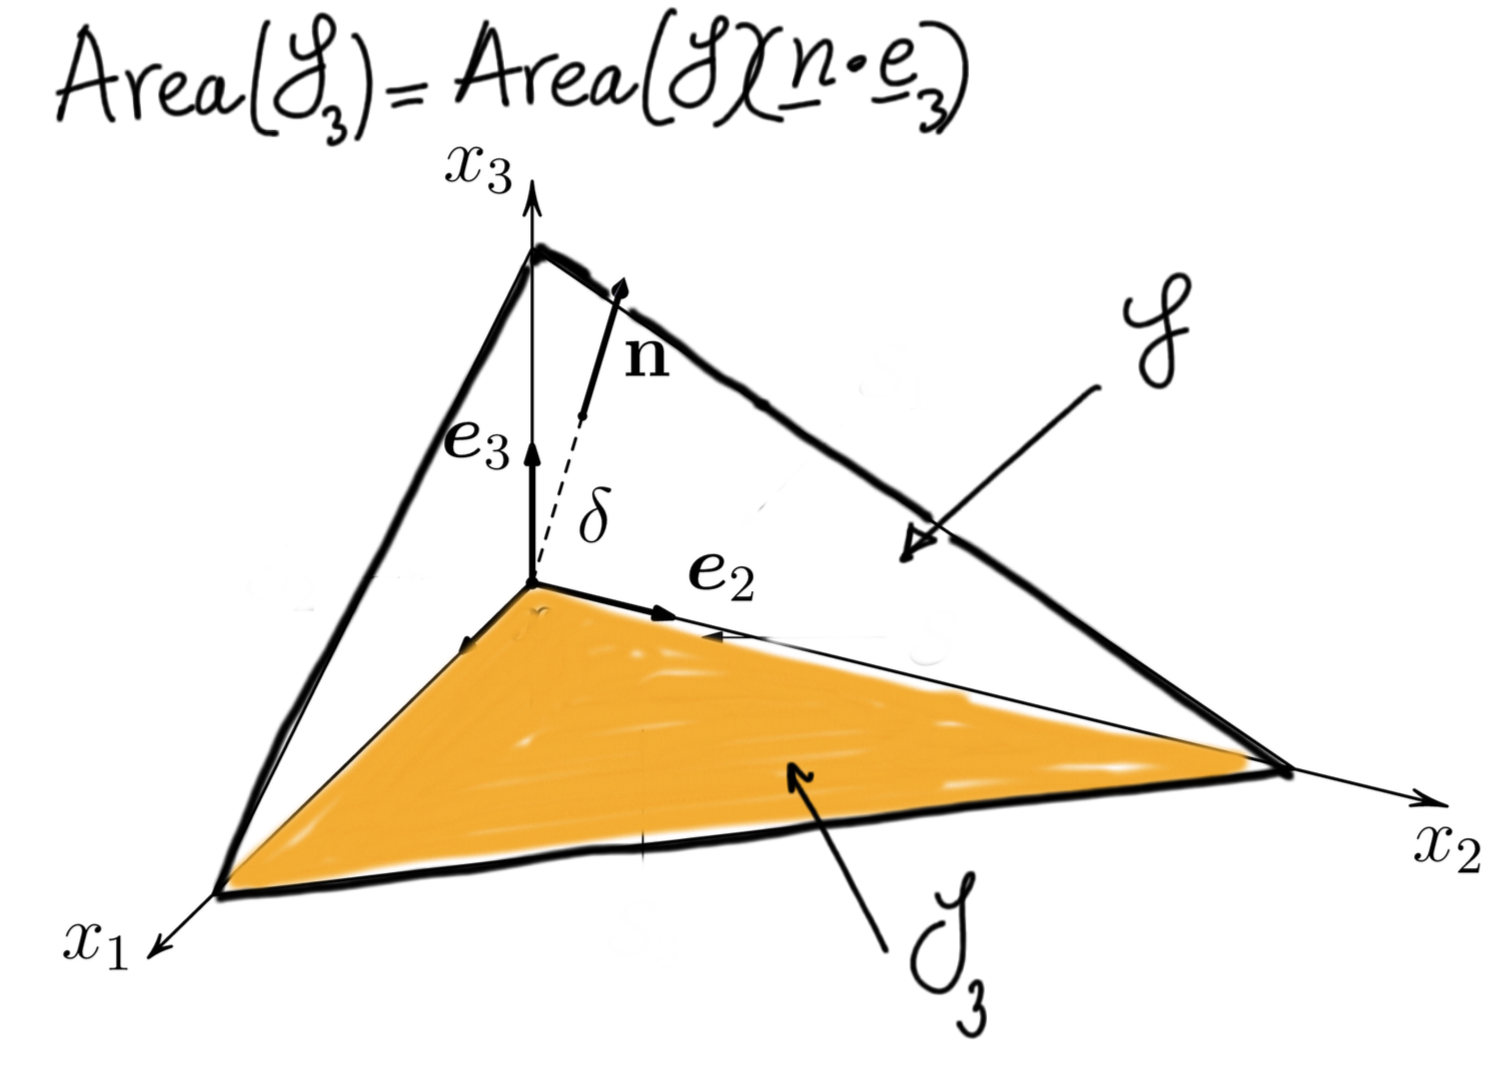
\includegraphics[width=\textwidth]{0bce64984c5c777909426f1b4db66ca6-v2xF77ePgG}
     \end{subfigure}
     \hfill
     \begin{subfigure}[b]{0.3\textwidth}
         \centering
         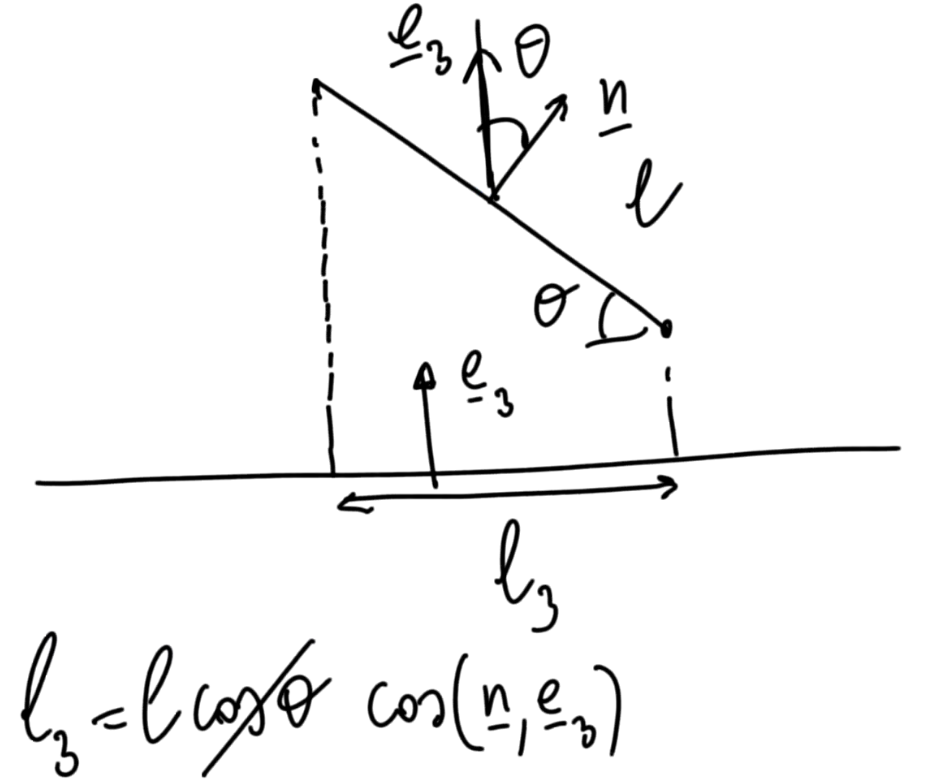
\includegraphics[width=\textwidth]{c8d471d6dc23ed5e0bee5afbe00c2756-5XM3NXdjmS}
     \end{subfigure}
     \hfill
\end{figure}
\FloatBarrier

analogamente per le altre facce

\begin{figure}[htpb]
     \centering
     \hfill
     \begin{subfigure}[b]{0.35\textwidth}
         \centering
         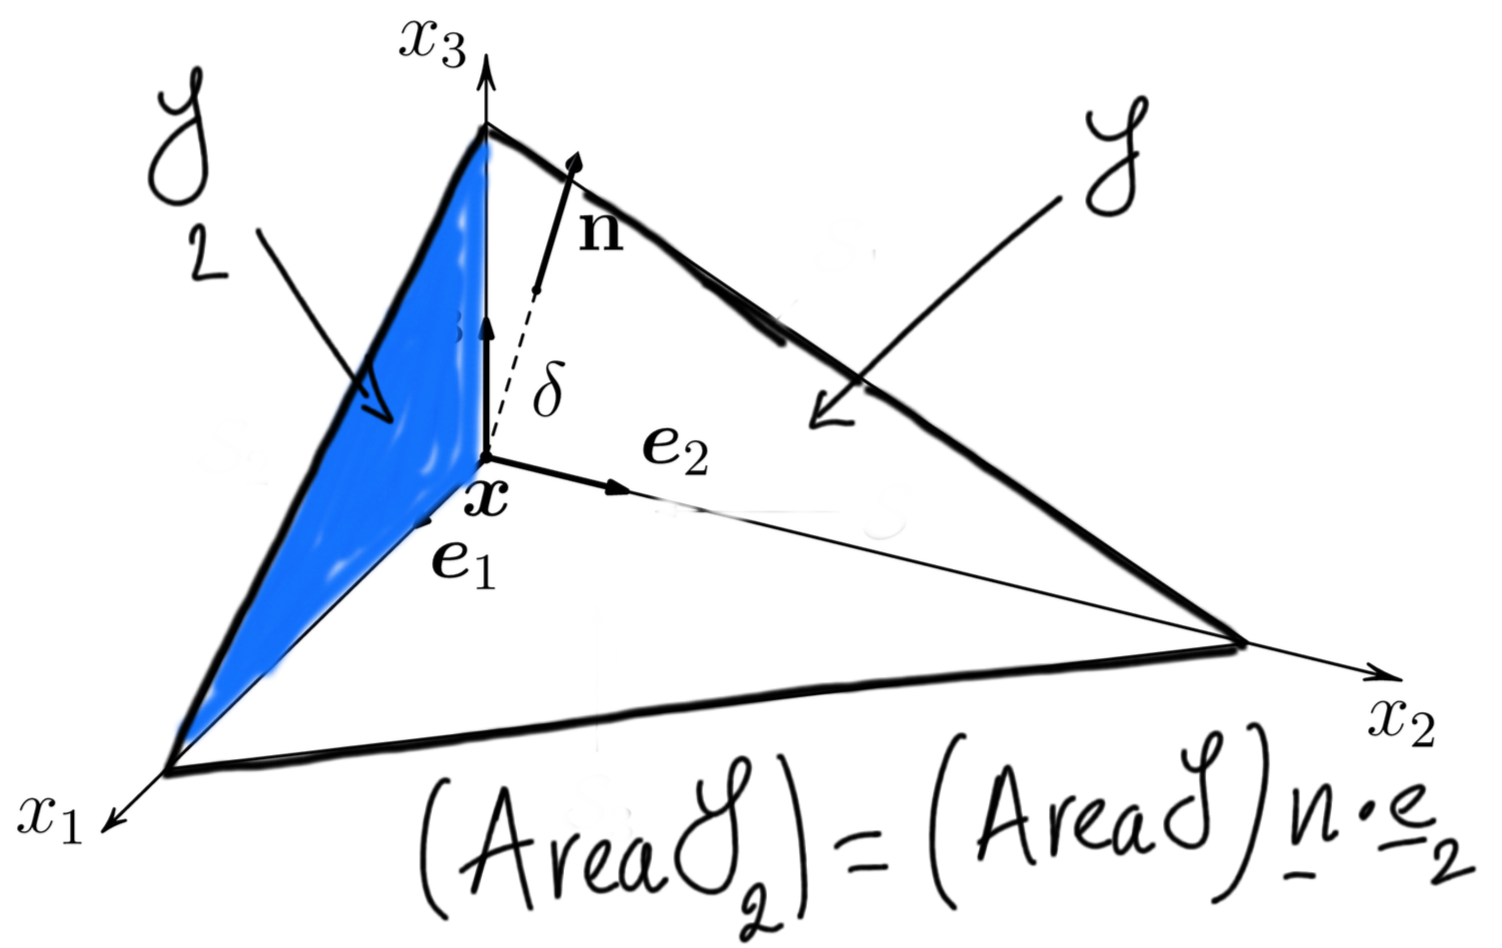
\includegraphics[width=\textwidth]{643fe22c279466a57b7e61a17b0096ae-vvHslRp3gY}
     \end{subfigure}
     \hfill
     \begin{subfigure}[b]{0.35\textwidth}
         \centering
         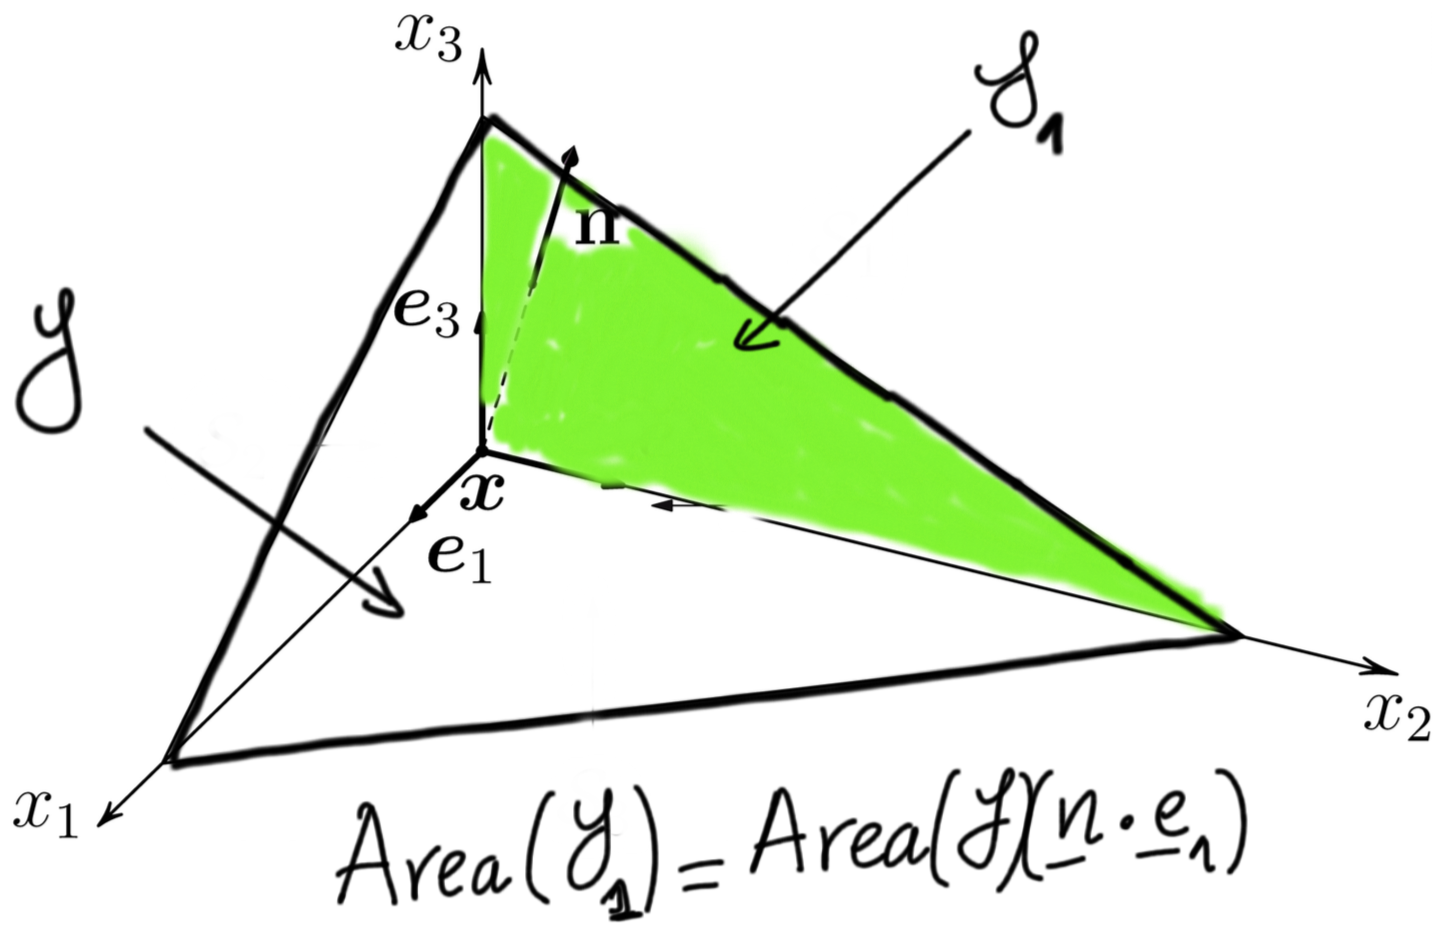
\includegraphics[width=\textwidth]{7cc1870c762f1de241ed7e7dcba96171-fG6hyVKATs}
     \end{subfigure}
     \hfill
\end{figure}
\FloatBarrier

Ovvero
\begin{equation*}
\mathrm{Area}(\mathcal{S}_{i}) =(\mathbf{n} \cdotp \mathbf{e}_{i})\mathrm{Area}(\mathcal{S}) \ \ \Rightarrow \ \ \frac{\mathrm{Area}(\mathcal{S}_{i})}{\mathrm{Area}(\mathcal{S})} =\mathbf{n} \cdotp \mathbf{e}_{i}
\end{equation*}
\textbf{Scriviamo la prima equazione cardinale.}
\begin{equation*}
\mathbf{R} =\dot{\mathbf{Q}}
\end{equation*}
\begin{itemize}
\item Abbiamo le forze di volume

\begin{equation*}
\int _{\mathcal{R}}\mathbf{b} dV_{x}
\end{equation*}
\item Abbiamo le forze di superficie
\begin{itemize}
\item sulla faccia $\mathcal{S}_{1}$\begin{equation*}
\int _{\mathcal{S}_{1}}\mathbf{s}(\mathbf{x} ,-\mathbf{e}_{1}) dAx
\end{equation*}infatti $-\mathbf{e}_{1}$ punta verso l'esterno, notiamo che qui $\mathbf{x}$ è generico, non fissato. Analoghe le altre due facce
\item sulla faccia $\mathcal{S}$\begin{equation*}
\int _{\mathcal{S}}\mathbf{s}(\mathbf{x} ,\mathbf{n}) dAx
\end{equation*}
\end{itemize}
\end{itemize}

Allora la risultante è
\begin{equation*}
\mathbf{R} =\int _{\mathcal{R}}\mathbf{b} dV_{x} +\sum\limits ^{3}_{i=1}\int _{\mathcal{S}_{i}}\mathbf{s}(\mathbf{x} ,-\mathbf{e}_{i}) dAx+\int _{\mathcal{S}}\mathbf{s}(\mathbf{x} ,\mathbf{n}) dAx
\end{equation*}
La derivata della quantità di moto è
\begin{equation*}
\dot{\mathbf{Q}} =\int _{\mathcal{R}} \rho \mathbf{a} dV_{x}
\end{equation*}
Siamo pronti per scrivere la I equazione cardinale
\begin{align*}
\int _{\mathcal{R}}\mathbf{b} dV_{x} +\sum\limits ^{3}_{i=1}\int _{\mathcal{S}_{i}}\mathbf{s}(\mathbf{x} ,-\mathbf{e}_{i}) dAx+\int _{\mathcal{S}}\mathbf{s}(\mathbf{x} ,\mathbf{n}) dAx & =\int _{\mathcal{R}} \rho \mathbf{a} dV_{x}\\
\int _{\mathcal{R}}\mathbf{b}^{*} dV_{x} +\sum\limits ^{3}_{i=1}\int _{\mathcal{S}_{i}}\mathbf{s}(\mathbf{x} ,-\mathbf{e}_{i}) dAx+\int _{\mathcal{S}}\mathbf{s}(\mathbf{x} ,\mathbf{n}) dAx & =0\ \ \ \ \ \ \ \ \mathbf{b^{*}} =\mathbf{b} -\rho \mathbf{a}
\end{align*}
Ricordiamo due proprietà
\begin{equation*}
\delta \rightarrow 0\ \ \frac{\mathrm{Vol}(\mathcal{R})}{\mathrm{Area}(\mathcal{S})} \sim \frac{c_{1} \delta ^{3}}{c_{2} \delta ^{2}}\rightarrow 0\ \ \ \ \ \ \ \ \frac{\mathrm{Area}(\mathcal{S}_{i})}{\mathrm{Area}(\mathcal{S})} =\mathbf{n} \cdotp \mathbf{e}_{i}
\end{equation*}


Dividiamo tutto per $\mathrm{Area}(\mathcal{S})$ e facciamo il limite per $\delta \rightarrow 0$ di ciascun termine
\begin{itemize}
\item Primo termine\begin{equation*}
\frac{\int _{\mathcal{R}}\mathbf{b}^{*} dV_{x}}{\mathrm{Area}(\mathcal{S})} =\frac{\int _{\mathcal{R}}\mathbf{b}^{*} dV_{x}}{\mathrm{Vol}(\mathcal{S})} \cdotp \frac{\mathrm{Vol}(\mathcal{S})}{\mathrm{Area}(\mathcal{S})}\rightarrow \mathbf{b}^{*}(\mathbf{x}) \cdotp 0=0
\end{equation*}
\item Secondo termine. Usiamo la dipendenza continua da $\mathbf{x}$\begin{equation*}
\frac{\int _{\mathcal{S}_{i}}\mathbf{s}(\mathbf{x} ,-\mathbf{e}_{i}) dAx}{\mathrm{Area}(\mathcal{S})} =\frac{\int _{\mathcal{S}_{i}}\mathbf{s}\left(\overbrace{\mathbf{x}}^{\text{generico}} ,-\mathbf{e}_{i}\right) dAx}{\mathrm{Area}(\mathcal{S}_{i})} \cdotp \frac{\mathrm{Area}(\mathcal{S}_{i})}{\mathrm{Area}(\mathcal{S})}\rightarrow \mathbf{s}\left(\overbrace{\mathbf{x}}^{\text{dell'origine}} ,-\mathbf{e}_{i}\right)(\mathbf{n} \cdotp \mathbf{e}_{i})
\end{equation*}
\item Terzo termine\begin{equation*}
\frac{\int _{\mathcal{S}}\mathbf{s}(\mathbf{x} ,\mathbf{n}) dAx}{\mathrm{Area}(\mathcal{S})}\rightarrow \mathbf{s}(\mathbf{x} ,\mathbf{n})
\end{equation*}
\end{itemize}

Tutto tende a
\begin{gather*}
\begin{array}{ c c c c }
\int _{\mathcal{R}}\mathbf{b}^{*} dV_{x} & +\sum\limits ^{3}_{i=1}\int _{\mathcal{S}_{i}}\mathbf{s}(\mathbf{x} ,-\mathbf{e}_{i}) dAx & +\int _{\mathcal{S}}\mathbf{s}(\mathbf{x} ,\mathbf{n}) dAx & =0\\
\downarrow  & \downarrow  & \downarrow  & \\
0 & +\sum\limits ^{3}_{i=1}\mathbf{s}(\mathbf{x} ,-\mathbf{e}_{i})(\mathbf{n} \cdotp \mathbf{e}_{i}) & +\mathbf{s}(\mathbf{x} ,\mathbf{n}) & =0
\end{array}\\
\Rightarrow \ \ \mathbf{s}(\mathbf{x} ,\mathbf{n}) =-\sum\limits ^{3}_{i=1}\mathbf{s}(\mathbf{x} ,-\mathbf{e}_{i})(\mathbf{n} \cdotp \mathbf{e}_{i})
\end{gather*}
Questa è una funzione continua in $\mathbf{n}$! Ma avevamo supposto $\mathbf{n}$ nel primo ottante!



\textit{Snodo importante che gli studenti di solito non capiscono.}

Qualunque $\mathbf{n}$ scelgo nella sfera unitaria, lui sarà nel primo ottante di \textbf{qualche} terna $\hat{\mathbf{e}}_{i}$!
\begin{equation*}
\mathbf{s}(\mathbf{x} ,\mathbf{n}) =-\sum\limits ^{3}_{i=1}\mathbf{s}(\mathbf{x} ,-\hat{\mathbf{e}}_{i})(\mathbf{n} \cdotp \hat{\mathbf{e}}_{i})
\end{equation*}
Quindi $\mathbf{s}$ dipende da $\mathbf{n}$ \textbf{con continuità!}

Grazie a questa continuità, possiamo fare il limite
\begin{equation*}
\begin{aligned}
\mathbf{s}(\mathbf{x} ,\mathbf{n}) & =-\sum\limits ^{3}_{i=1}\mathbf{s}(\mathbf{x} ,-\mathbf{e}_{i})(\mathbf{n} \cdotp \mathbf{e}_{i})\\
 & \Downarrow \mathbf{n}\rightarrow \mathbf{e}_{1}\\
\mathbf{s}(\mathbf{x} ,\mathbf{e}_{1}) & =-\mathbf{s}(\mathbf{x} ,-\mathbf{e}_{1})
\end{aligned}
\end{equation*}
ma $\mathbf{e}_{1}$ è un versore qualunque, abbiamo quindi \textit{dedotto} il principio di azione e reazione!
\begin{equation*}
\boxed{\mathbf{s}(\mathbf{x} ,\mathbf{n}) =-\mathbf{s}(\mathbf{x} ,-\mathbf{n})}
\end{equation*}
Vogliamo mostrare che vale (\underline{\textbf{con la stessa}} terna $\mathbf{e}_{i}$) per \underline{\textbf{tutti}} gli $\mathbf{n}$

Supponiamo di prendere un $\mathbf{n}$ non sul primo ottante, ma tale che
\begin{equation*}
\mathbf{n} \cdotp \mathbf{e}_{1}\textcolor[rgb]{0.82,0.01,0.11}{< } 0\ \ \ \ \mathbf{n} \cdotp \mathbf{e}_{2}  >0\ \ \ \ \mathbf{n} \cdotp \mathbf{e}_{3}  >0
\end{equation*}
definiamo una nuova terna
\begin{equation*}
\overline{\mathbf{e}}_{1} =\textcolor[rgb]{0.82,0.01,0.11}{-}\mathbf{e}_{1} \ \ \ \ \overline{\mathbf{e}}_{2} =\mathbf{e}_{2} \ \ \ \ \overline{\mathbf{e}}_{3} =\mathbf{e}_{3}
\end{equation*}
ma quindi, grazie al principio di azione e reazione possiamo ricondurci alla terna principale
\begin{equation*}
\begin{aligned}
\mathbf{s}(\mathbf{x} ,\mathbf{n}) & =\sum\limits ^{3}_{i=1}\mathbf{s}(\mathbf{x} ,\overline{\mathbf{e}}_{i})(\mathbf{n} \cdotp \overline{\mathbf{e}}_{i})\\
 & =\mathbf{s}(\mathbf{x} ,\overline{\mathbf{e}}_{1})(\mathbf{n} \cdotp \overline{\mathbf{e}}_{1}) +\mathbf{s}(\mathbf{x} ,\overline{\mathbf{e}}_{2})(\mathbf{n} \cdotp \overline{\mathbf{e}}_{2}) +\mathbf{s}(\mathbf{x} ,\overline{\mathbf{e}}_{3})(\mathbf{n} \cdotp \overline{\mathbf{e}}_{3})\\
 & =\mathbf{s}(\mathbf{x} ,-\mathbf{e}_{1})(\mathbf{n} \cdotp -\mathbf{e}_{1}) +\mathbf{s}(\mathbf{x} ,\mathbf{e}_{2})(\mathbf{n} \cdotp \mathbf{e}_{2}) +\mathbf{s}(\mathbf{x} ,\mathbf{e}_{3})(\mathbf{n} \cdotp \mathbf{e}_{3})\\
 & =\mathbf{s}(\mathbf{x} ,\mathbf{e}_{1})(\mathbf{n} \cdotp \mathbf{e}_{1}) +\mathbf{s}(\mathbf{x} ,\mathbf{e}_{2})(\mathbf{n} \cdotp \mathbf{e}_{2}) +\mathbf{s}(\mathbf{x} ,\mathbf{e}_{3})(\mathbf{n} \cdotp \mathbf{e}_{3})
\end{aligned}
\end{equation*}
possiamo quindi scrivere la forma generale del tensore degli sforzi grazie al prodotto tensoriale\footnote{$(\mathbf{a} \otimes \mathbf{b})\mathbf{v} =(\mathbf{b} \cdotp \mathbf{v})\mathbf{a}$.}
\begin{equation*}
\boxed{\mathbf{s}(\mathbf{x} ,\mathbf{n}) =\sum\limits ^{3}_{i=1}(\mathbf{n} \cdotp \mathbf{e}_{i})\mathbf{s}(\mathbf{x} ,\mathbf{e}_{i}) =\left[\sum\limits ^{3}_{i=1}\mathbf{s}(\mathbf{x} ,\mathbf{e}_{i}) \otimes \mathbf{e}_{i}\right]\mathbf{n} =\mathbf{T}(\mathbf{x})\mathbf{n}}
\end{equation*}
per \textbf{ogni} $\mathbf{n}$ con terna $\mathbf{e}_{i}$ \textbf{generica}, c'è \textbf{dipendenza lineare} da $\mathbf{n}$!
\begin{equation*}
\qed 
\end{equation*}
\section{Proprietà del tensore degli sforzi}

Sottintendiamo $\mathbf{x}$.

Ricordiamo la relazione di Cauchy
\begin{equation*}
s(\mathbf{n}) =\mathbf{Tn} =\sum _{i}(\mathbf{n} \cdotp \mathbf{e}_{i})\mathbf{s}(\mathbf{e}_{i})
\end{equation*}
In generale lo sforzo non è perpendolare alla normale
\begin{equation*}
\sum _{i}(\mathbf{n} \cdotp \mathbf{e}_{i})\mathbf{s}(\mathbf{e}_{i}) =\sum _{i} n_{i}\mathbf{s}(\mathbf{e}_{i}) =n_{1}\mathbf{s}(\mathbf{e}_{1}) +n_{2}\mathbf{s}(\mathbf{e}_{2}) +n_{3}\mathbf{s}(\mathbf{e}_{3})
\end{equation*}
si riduce il calcolo di $\mathbf{s}$ al suo valore lungo le tre componenti di $\mathbf{n}$


\begin{figure}[htpb]
     \centering
     \begin{subfigure}[b]{0.3\textwidth}
         \centering
         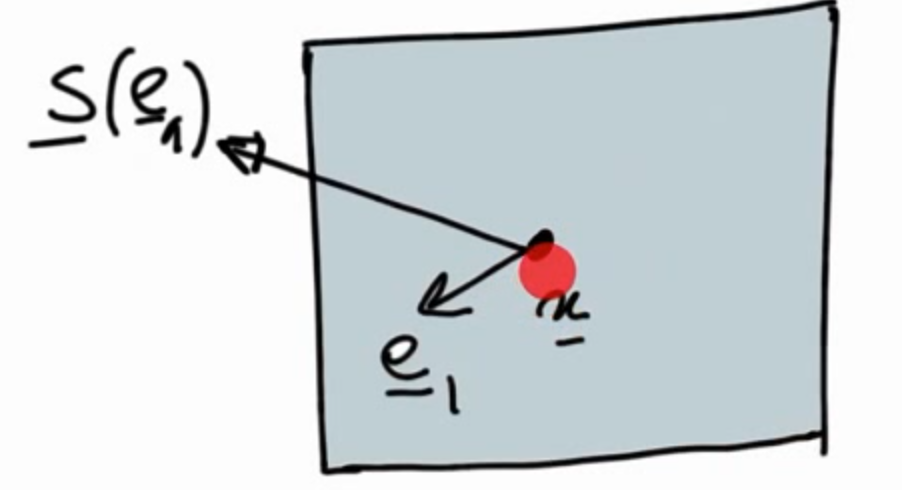
\includegraphics[width=\textwidth]{9b7dab8fdf5aefe607e6e3cc737f5c71-zkSKd1j84w}
     \end{subfigure}
     \hfill
     \begin{subfigure}[b]{0.3\textwidth}
         \centering
         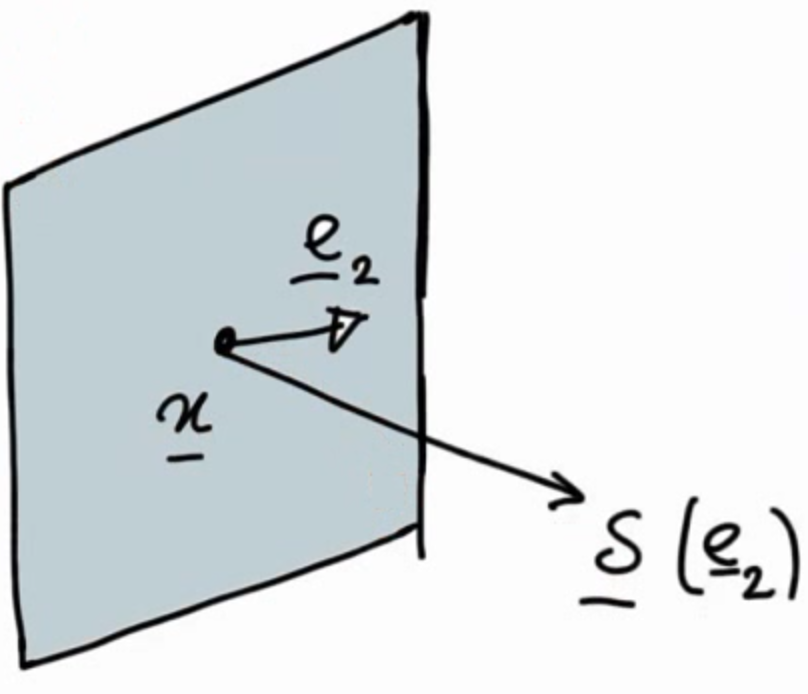
\includegraphics[width=\textwidth]{abf9e33612f83c0690f821f17beddbcc-WYjIv2gsZd}
     \end{subfigure}
     \hfill
     \begin{subfigure}[b]{0.3\textwidth}
         \centering
         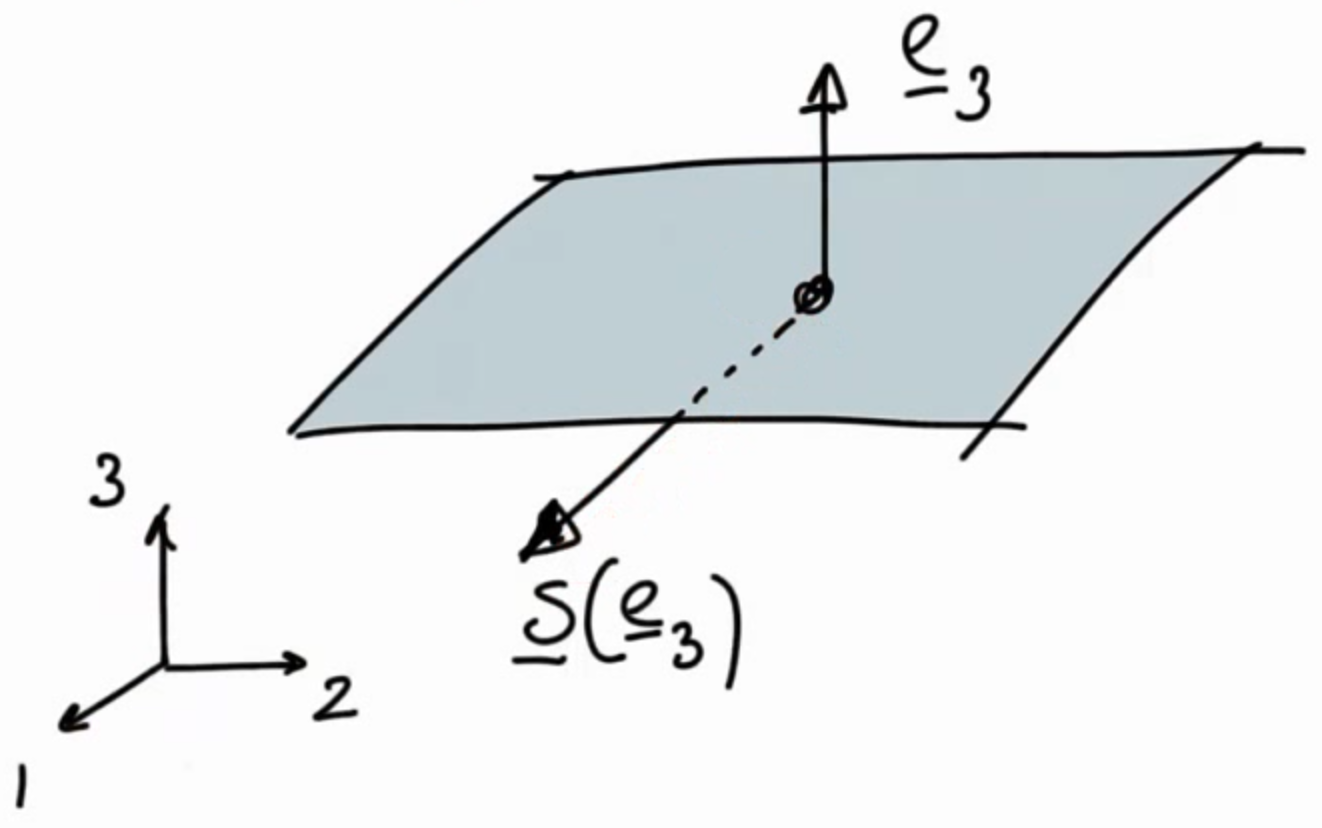
\includegraphics[width=\textwidth]{27a182fb6c39f9ddaef3390d5b6ad56c-gzi3kjO9xo}
     \end{subfigure}
\end{figure}
\FloatBarrier

Ma noi sappiamo che
\begin{equation*}
T_{ij} =\mathbf{e}_{i} \cdotp \mathbf{Te}_{j} =\mathbf{e}_{i} \cdotp \mathbf{s}(\mathbf{e}_{j})
\end{equation*}
Allora deduciamo che lungo le colonne di $\mathbf{T}$ ci sono le componenti dello sforzo agente sulla superficie normale a quella direzione
\begin{equation*}
\begin{array}{ c }
T_{11} =\mathbf{e}_{1} \cdotp \mathbf{s}(\mathbf{e}_{1})\\
T_{21} =\mathbf{e}_{2} \cdotp \mathbf{s}(\mathbf{e}_{1})\\
T_{31} =\mathbf{e}_{3} \cdotp \mathbf{s}(\mathbf{e}_{1})
\end{array} \ \ \Rightarrow \ \ \mathbf{T} =
\left[\begin{array}{c|c|c}
T_{11} & T_{12} & T_{13}\\
T_{21} & T_{22} & T_{23}\\
T_{31} & T_{33} & T_{33}
\end{array}\right] =
\left[\begin{array}{c|c|c}
\mathbf{s}(\mathbf{e}_{1}) & \mathbf{s}(\mathbf{e}_{2}) & \mathbf{s}(\mathbf{e}_{3})\\
\end{array}\right]
\end{equation*}
\begin{itemize}
\item $\mathbf{Tn} \cdotp \mathbf{n}$ è la componente normale dello sforzo
\item $(\mathbf{Tn} \cdotp \mathbf{n})\mathbf{n}$ è lo sforzo normale
\item $\mathbf{Tn} -(\mathbf{Tn} \cdotp \mathbf{n})\mathbf{n}$ è lo sforzo di taglio
\end{itemize}

\fg{0.2}{3b996ed400816581aef9e398849744d4-qfdZFqSGu4}

Essendo $\mathbf{T} \in \mathrm{Sym}$ si può diagonalizzare
\begin{equation*}
\text{rispetto a} \ \hat{\mathbf{e}}_{i}( \exists ) \ \ \Rightarrow \ \ \mathbf{T} =\begin{bmatrix}
\sigma _{1} & 0 & 0\\
0 & \sigma _{2} & 0\\
0 & 0 & \sigma _{3}
\end{bmatrix} \ \ \ \ \mathbf{T}\hat{\mathbf{e}}_{i} =\sigma _{i}\hat{\mathbf{e}}_{i}
\end{equation*}
sulle superfici perpendicolari a $\hat{\mathbf{e}}_{i}$ lo sforzo è puramente normale, \textbf{non c'è sforzo di taglio}.
\begin{itemize}
\item \textbf{Direzioni principali di sforzo} $\hat{\mathbf{e}}_{i}$
\item \textbf{Sforzi principali} $\sigma _{i}$
\end{itemize}
\subsection{Cubo degli sforzi}

\fg{0.3}{f01b25c4c4087680b2b04d1753bb8000-8BEsS0WeFc}

\section{I equazione "indefinita" di moto dei continui}

Scriviamo la I Equazione Cardinale per una regione $\mathcal{P}_{t}$ e sottintendiamo la dipendenza dei termini da $\mathbf{x}$
\begin{align*}
\int _{\mathcal{P}_{t}}\mathbf{b} dV_{x} +\int _{\partial \mathcal{P}_{t}}\mathbf{s}(\mathbf{x} ,\mathbf{n}) dAx & =\int _{\mathcal{P}_{t}} \rho \mathbf{a} dV_{x}\\
\int _{\mathcal{P}_{t}}\mathbf{b} dV_{x} +\int _{\partial \mathcal{P}_{t}}\mathbf{Tn} dAx & =\int _{\mathcal{P}_{t}} \rho \mathbf{a} dV_{x}
\end{align*}
Vale il Teorema della divergenza per tensori
\begin{align*}
\int _{\mathcal{R}}\mathrm{div}(\mathbf{w}) dV_{x} & =\int _{\partial \mathcal{R}}\mathbf{w} \cdotp \mathbf{n} dA_{x}\\
\int _{\mathcal{R}}\mathrm{div}(\mathbf{T}) dV_{x} & =\int _{\partial \mathcal{R}}\mathbf{Tn} dA_{x}
\end{align*}
quindi
\begin{align*}
\int _{\mathcal{P}_{t}}\mathbf{b} dV_{x} +\int _{\partial \mathcal{P}_{t}}\mathbf{T}(\mathbf{x})\mathbf{n}(\mathbf{x}) dAx & =\int _{\mathcal{P}_{t}} \rho \mathbf{a} dV_{x}\\
\int _{\mathcal{P}_{t}}\mathbf{b} dV_{x} +\int _{\mathcal{P}_{t}}\mathrm{div}(\mathbf{T}) dVx & =\int _{\mathcal{P}_{t}} \rho \mathbf{a} dV_{x}\\
\int _{\mathcal{P}_{t}}[\mathbf{b} +\mathrm{div}(\mathbf{T}) -\rho \mathbf{a}] dVx & =0,\ \ \ \ \forall \mathcal{P}_{t}
\end{align*}
essendo nullo per ogni regione di integrazione deve essere nulla l'integranda
\begin{gather*}
\boxed{\mathbf{b} +\mathrm{div}(\mathbf{T}) =\rho \mathbf{a}}\\
\qed 
\end{gather*}
\section{II equazione "indefinita" di moto dei continui}

Scriviamo la II Equazione Cardinale per una regione $\mathcal{P}_{t}$
\begin{align*}
\int _{\mathcal{P}_{t}}(\mathbf{x} -O) \land \mathbf{b} dV_{x} +\int _{\partial \mathcal{P}_{t}}(\mathbf{x} -\mathbf{O}) \land \mathbf{s}(\mathbf{x} ,\mathbf{n}) dAx & =\int _{\mathcal{P}_{t}}(\mathbf{x} -O) \land \rho \mathbf{a} dV_{x}\\
\int _{\mathcal{P}_{t}}(\mathbf{x} -O) \land \mathbf{b} dV_{x} +\int _{\partial \mathcal{P}_{t}}(\mathbf{x} -\mathbf{O}) \land \mathbf{T}(\mathbf{x})\mathbf{n}(\mathbf{x}) dAx & =\int _{\mathcal{P}_{t}}(\mathbf{x} -O) \land \rho \mathbf{a} dV_{x}\\
\int _{\mathcal{P}_{t}}(\mathbf{x} -O) \land \underbrace{(\mathbf{b} -\rho \mathbf{a})}_{\mathbf{b}^{*}} dV_{x} +\int _{\partial \mathcal{P}_{t}}(\mathbf{x} -\mathbf{O}) \land \mathbf{T}(\mathbf{x})\mathbf{n}(\mathbf{x}) dAx & =0
\end{align*}
moltiplichiamo scalarmente per un vettore $\mathbf{w}$
\begin{equation*}
\mathbf{w} \cdotp \int _{\mathcal{P}_{t}}(\mathbf{x} -O) \land \mathbf{b}^{*} dV_{x} +\mathbf{w} \cdotp \int _{\partial \mathcal{P}_{t}}(\mathbf{x} -\mathbf{O}) \land \mathbf{T}(\mathbf{x})\mathbf{n}(\mathbf{x}) dAx=0
\end{equation*}
grazie alle proprietà del prodotto misto\footnote{$a\cdotp b\land c=a\land b\cdotp c$}
\begin{equation*}
\int _{\mathcal{P}_{t}}\mathbf{\textcolor[rgb]{0.82,0.01,0.11}{w}}\textcolor[rgb]{0.82,0.01,0.11}{\land }\textcolor[rgb]{0.82,0.01,0.11}{(}\mathbf{\textcolor[rgb]{0.82,0.01,0.11}{x}}\textcolor[rgb]{0.82,0.01,0.11}{-O}\textcolor[rgb]{0.82,0.01,0.11}{)} \cdotp \mathbf{b}^{*} dV_{x} +\int _{\partial \mathcal{P}_{t}}\mathbf{\textcolor[rgb]{0.82,0.01,0.11}{w}}\textcolor[rgb]{0.82,0.01,0.11}{\land }\textcolor[rgb]{0.82,0.01,0.11}{(}\mathbf{\textcolor[rgb]{0.82,0.01,0.11}{x}}\textcolor[rgb]{0.82,0.01,0.11}{-O}\textcolor[rgb]{0.82,0.01,0.11}{)} \cdotp \mathbf{T}(\mathbf{x})\mathbf{n}(\mathbf{x}) dAx=0
\end{equation*}
possiamo chiamare $\mathbf{\textcolor[rgb]{0.82,0.01,0.11}{w}}\textcolor[rgb]{0.82,0.01,0.11}{\land }\textcolor[rgb]{0.82,0.01,0.11}{(}\mathbf{\textcolor[rgb]{0.82,0.01,0.11}{x}}\textcolor[rgb]{0.82,0.01,0.11}{-O}\textcolor[rgb]{0.82,0.01,0.11}{)}\textcolor[rgb]{0.82,0.01,0.11}{=}\mathbf{\textcolor[rgb]{0.82,0.01,0.11}{u}}\textcolor[rgb]{0.82,0.01,0.11}{(}\mathbf{\textcolor[rgb]{0.82,0.01,0.11}{x}}\textcolor[rgb]{0.82,0.01,0.11}{)}$. A $\mathbf{w}$ corrisponde un tensore antisimmetrico $\mathbf{W}$ tale che $\mathbf{u}(\mathbf{x}) =\mathbf{W}(\mathbf{x} -O)$. Deduciamo per il passaggio successivo questa cosa
\begin{align*}
\frac{\mathbf{u}(\mathbf{x} +\mathbf{h}) -\mathbf{u}(\mathbf{x})}{\mathbf{h}} & =\frac{\mathbf{W}(\mathbf{x} +\mathbf{h} -O) -\mathbf{W}(\mathbf{x} -O)}{\mathbf{h}}\\
 & =\frac{\cancel{\mathbf{W}(\mathbf{x} -O)} +\mathbf{Wh} -\cancel{\mathbf{W}(\mathbf{x} -O)}}{\mathbf{h}} =\mathbf{W}
\end{align*}
Se prendiamo il limite per $\mathbf{h}\rightarrow \mathbf{0}$ otteniamo la derivata nello spazio, cioè il gradiente, del primo termine (mentre il secondo non dipende da $\mathbf{h}$)
\begin{equation*}
\mathbf{W} =\lim\limits _{\mathbf{h}\rightarrow \mathbf{0}}\frac{\mathbf{u}(\mathbf{x} +\mathbf{h}) -\mathbf{u}(\mathbf{x})}{\mathbf{h}} =\mathrm{grad}\mathbf{u}
\end{equation*}
sostituiamo e sottintendiamo la dipendenza da $\mathbf{x}$ per alleggerire la notazione
\begin{align*}
\int _{\mathcal{P}_{t}}\mathbf{\textcolor[rgb]{0.82,0.01,0.11}{u}} \cdotp \mathbf{b}^{*} dV_{x} +\int _{\partial \mathcal{P}_{t}}\mathbf{\textcolor[rgb]{0.82,0.01,0.11}{u}} \cdotp \mathbf{Tn} dAx & =0\\
\int _{\mathcal{P}_{t}}\mathbf{u} \cdotp \mathbf{b}^{*} dV_{x} +\int _{\partial \mathcal{P}_{t}}\mathbf{T}^{T}\mathbf{u} \cdotp \mathbf{n} dAx & =0\\
\int _{\mathcal{P}_{t}}\mathbf{u} \cdotp \mathbf{b}^{*} dV_{x} +\int _{\mathcal{P}_{t}}\mathrm{div}\left(\mathbf{T}^{T}\mathbf{u}\right) dV_{x} & =0
\end{align*}
analizziamo il termine della divergenza
\begin{equation*}
\begin{aligned}
\mathrm{div}\left(\mathbf{T}^{T}\mathbf{u}\right) & =\sum _{k,i}\left( T^{T}_{ik} u_{k}\right)_{,i} =\sum _{k,i}( T_{ki} u_{k})_{,i} & \\
 & =\sum _{k,i} T_{ki,i} u_{k} +T_{ki} u_{k,i} & \\
 & =(\mathrm{div}\mathbf{T}) \cdotp \mathbf{u} +\mathbf{T} \cdotp \mathrm{grad}\mathbf{u} & \text{(valido sempre fino a qui)}\\
 & =(\mathrm{div}\mathbf{T}) \cdotp \mathbf{u} +\mathbf{T} \cdotp \mathbf{W} & \text{(risultato di prima)}
\end{aligned}
\end{equation*}
Sostituiamo
\begin{equation*}
\begin{aligned}
\int _{\mathcal{P}_{t}}\mathbf{u} \cdotp \mathbf{b}^{*} dV_{x} +\int _{\mathcal{P}_{t}}\mathrm{div}\left(\mathbf{T}^{T}\mathbf{u}\right) dV_{x} & =0\\
\int _{\mathcal{P}_{t}}\mathbf{u} \cdotp \mathbf{b}^{*} dV_{x} +\int _{\mathcal{P}_{t}}(\mathrm{div}\mathbf{T} \cdotp \mathbf{u} +\mathbf{T} \cdotp \mathbf{W}) dV_{x} & =0\\
\int _{\mathcal{P}_{t}}\mathbf{u} \cdotp \left(\mathbf{b}^{*} +\mathrm{div}\mathbf{T}\right) dV_{x} +\int _{\mathcal{P}_{t}}(\mathbf{T} \cdotp \mathbf{W}) dV_{x} & =0\\
\int _{\mathcal{P}_{t}}\mathbf{u} \cdotp \underbrace{(\mathbf{b} -\rho \mathbf{a} +\mathrm{div}\mathbf{T})}_{=0\ \text{(I eq. indefinita)}} dV_{x} +\int _{\mathcal{P}_{t}}(\mathbf{T} \cdotp \mathbf{W}) dV_{x} & =0\\
\int _{\mathcal{P}_{t}}(\mathbf{T} \cdotp \mathbf{W}) dV_{x} & =0\ \ \forall \mathcal{P}_{t} ,\forall \mathbf{W} \in \mathrm{Skw}
\end{aligned}
\end{equation*}
essendo nullo per ogni regione di integrazione deduciamo che deve essere nulla l'integranda
\begin{equation*}
\mathbf{T} \cdotp \mathbf{W} =0
\end{equation*}
inoltre $\mathbf{W}$ è un arbitrario tensore antisimmetrico. Essendo $\mathbf{T}$ ortogonale a tutti i tensori antisimmetrici, non può che essere simmetrico!\footnote{Gli spazi dei tensori simmetrici e antisimmetrici sono ortogonali.}
\begin{equation*}
\boxed{\mathbf{T} =\mathbf{T}^{T}}
\end{equation*}
In conclusione abbiamo che\footnote{Si noti che la dimostrazione della seconda \textit{dipende} dalla prima, quindi non si può considerare come un'equazione indipendente a sé stante derivante dai princìpi della fisica.}
\begin{equation*}
\begin{cases}
\mathbf{b} +\mathrm{div}(\mathbf{T}) =\rho \mathbf{a}\\
\mathbf{T} =\mathbf{T}^{T}
\end{cases} \ \ \forall (\mathbf{x} ,t) ,\forall \mathcal{B}_{t}
\end{equation*}
\textbf{Queste relazioni bastano a determinare il moto e gli sforzi, cioè il processo dinamico? No.}

Il moto $\mathbf{x} =\mathbf{f}(\mathbf{p} ,t)$ corrisponde a $3$ equazioni scalari, mentre gli sforzi corrispondono a $6$ equazioni (le sei componenti indipendenti di $\mathbf{T}$). Naturalmente $3+6=9$, mentre l'equazione indefinita $[\mathbf{b} +\mathrm{div}(\mathbf{T}) =\rho \mathbf{a}]$ ci dà solo $3$ equazioni.

È giusto che manchi qualcosa! Per completare la determinazione del moto bisogna specificare se stiamo parlando di corpi elastici, viscoelastici, ecc. tramite le cosiddette \textbf{relazioni costitutive}. Il discorso fatto fin'ora è puramente generale.
\section{Teorema dell'energia cinetica}

Proponiamo ora la dimostrazione del teorema dell'energia cinetica per i corpi continui. Sfruttiamo come primo passo il teorema che ci permette di portare all'interno dell'integrale la derivata temporale, dato che il campo da integrare è moltiplicato dalla densità (questo passaggio \textit{non} è in generale lecito).
\begin{align*}
T & =\frac{1}{2}\int _{\mathcal{P}_{t}} \rho \mathbf{v}^{2} dV_{x}\\
\frac{dT}{dt} & =\frac{1}{2}\int _{\mathcal{P}_{t}} \rho \left(\mathbf{v}^{2}\right)\dot{} dV_{x} =( *)\\
 & \\
 & (\mathbf{v} \cdotp \mathbf{v})\dot{} =\mathbf{a} \cdotp \mathbf{v} +\mathbf{v} \cdotp \mathbf{a} =2\mathbf{v} \cdotp \mathbf{a}\\
 & \rho \mathbf{a} =\mathbf{b} +\mathrm{div}\mathbf{T}\\
 & \\
( *) & =\int _{\mathcal{P}_{t}} \rho \mathbf{a} \cdotp \mathbf{v} dV_{x}\\
 & =\int _{\mathcal{P}_{t}}(\mathbf{b} +\mathrm{div}\mathbf{T}) \cdotp \mathbf{v} dV_{x}\\
 & =\underbrace{\int _{\mathcal{P}_{t}}\mathbf{b} \cdotp \mathbf{v} dV_{x}}_{\text{pot. forze di vol.}} +\int _{\mathcal{P}_{t}}\mathrm{div}\mathbf{T} \cdotp \mathbf{v} dV_{x}\\
 & =\Pi ^{\text{vol}} +\int _{\mathcal{P}_{t}}\mathrm{div}\mathbf{T} \cdotp \mathbf{v} dV_{x} =( **)\\
 & \\
 & \mathrm{div}\left(\mathbf{T}^{T}\mathbf{v}\right) =\mathrm{div}\mathbf{T} \cdotp \mathbf{v} +\mathbf{T} \cdotp \mathrm{grad}\mathbf{v}\\
 & \\
( **) & =\Pi ^{\text{vol}} +\int _{\mathcal{P}_{t}}\left(\mathrm{div}\left(\mathbf{T}^{T}\mathbf{v}\right) -\mathbf{T} \cdotp \mathrm{grad}\mathbf{v}\right) dV_{x}\\
 & =\Pi ^{\text{vol}} +\underbrace{\int _{\mathcal{P}_{t}}\mathrm{div}\left(\mathbf{T}^{T}\mathbf{v}\right) dV_{x}}_{\text{(teo. div.)}} -\int _{\mathcal{P}_{t}}\mathbf{T} \cdotp \mathrm{grad}\mathbf{v} dV_{x}\\
 & =\Pi ^{\text{vol}} +\int _{\partial \mathcal{P}_{t}}\mathbf{T}^{T}\mathbf{v} \cdotp \mathbf{n} dV_{x} -\int _{\mathcal{P}_{t}}\mathbf{T} \cdotp \mathrm{grad}\mathbf{v} dV_{x}\\
 & =\Pi ^{\text{vol}} +\int _{\partial \mathcal{P}_{t}}\mathbf{v} \cdotp \mathbf{Tn} dV_{x} -\int _{\mathcal{P}_{t}}\mathbf{T} \cdotp \mathrm{grad}\mathbf{v} dV_{x} \ \ \ \ \mathbf{Tn} \leftrightarrow \mathbf{s}(\mathbf{n})\\
 & =\Pi ^{\text{vol}} +\Pi ^{\text{contatto}} -\int _{\mathcal{P}_{t}}\mathbf{T} \cdotp \mathrm{grad}\mathbf{v} dV_{x} =( ***)
\end{align*}
Notiamo ora che $\mathrm{grad}\mathbf{v} =\mathbf{D} +\mathbf{W}$, che $\mathbf{W} \in \mathrm{Skw}$ e $\mathbf{T} \in \mathrm{Sym}$, ma dato che gli spazi dei tensori simmetrici e antisimmetrici sono ortogonali otteniamo $\mathbf{T} \cdotp \mathbf{W} =0$, rimane pertanto solo il termine in $\mathbf{D}$.
\begin{align*}
( ***) & =\Pi ^{\text{vol}} +\Pi ^{\text{contatto}} -\int _{\mathcal{P}_{t}}\mathbf{T} \cdotp \mathbf{D} dV_{x}\\
 & =\Pi ^{\text{vol}} +\Pi ^{\text{contatto}} +\Pi ^{\text{forze interne (sforzi)}}
\end{align*}
Riassumiamo il risultato
\begin{gather*}
\boxed{\dot{T} =\Pi ^{\text{vol}} +\Pi ^{\text{contatto}} +\Pi ^{\text{forze interne (sforzi)}}}\\
\qed 
\end{gather*}
\chapter{Relazioni costitutive e fluidi}

Sono le condizioni al contorno che completano le equazioni.

Potrei vincolare una certa parte del corpo a stare fermo sulla parete, oppure potrei vincolare la velocità, o potrei vincolarlo alla presenza di forze.

Una \underline{\textbf{classe costitutiva}} è una restrizione sull'insieme dei processi dinamici.



\textit{Esempio.}
\begin{itemize}
\item classe dei \textbf{corpi elastici:} $\mathbf{T} =\hat{\mathbf{T}}(\mathbf{F})$.

cioè $\mathbf{T}$ è una funzione nota del gradiente di deformazione
\item classe dei \textbf{corpi viscoelastici:} $\mathbf{T} =\hat{\mathbf{T}}(\mathbf{F} ,\dot{\mathbf{F}})$.

spesso questa dipendenza viene indicata come $\mathbf{T} =\hat{\mathbf{T}}(\mathbf{F} ,\mathbf{L})$, dato che $\mathbf{L} =\mathrm{grad}\mathbf{v} =\dot{\mathbf{F}}\mathbf{F}^{-1}$ e quindi vi è comunque dipendenza.
\end{itemize}



Stiamo entrando nel mondo empirico, quindi sarà comune fare una serie di ipotesi semplificative, ma comunque molto comuni nella pratica.

\fg{0.4}{231481073f1e43ca02eaac25cd487dd5-jn9ZcGnn9h}

\begin{oss}
Un tensore $\mathbf{T}$ è \textbf{isotropo} se $\mathbf{T} =\alpha \mathbf{I} ,\ \alpha \in \mathbb{R}$.

Un tensore $\mathbf{T}$ è \textbf{deviatorico} se $\mathrm{tr}(\mathbf{T}) =0$.

Ogni tensore può essere scomposto come somma di un tensore isotropo e uno deviatorico
\begin{equation*}
\boxed{\mathbf{T} =\alpha \mathbf{I} +\mathbf{T}_{0}}
\end{equation*}
\end{oss}
\textit{Dimostrazione.}

Bisogna determinare $\alpha $ e $\mathbf{T}_{0}$, e far vedere che $\mathbf{T}_{0}$ è deviatorico.
\begin{gather*}
\alpha :=\frac{1}{3}\mathrm{tr}(\mathbf{T}) \ \ \ \ \mathbf{T}_{0} :=\mathbf{T} -\alpha \mathbf{I}\\
\mathrm{tr}\mathbf{T}_{0} =\mathrm{tr}\mathbf{T} -\mathrm{tr}( \alpha \mathbf{I}) =\mathrm{tr}\mathbf{T} -\alpha \cdotp \mathrm{tr}\mathbf{I} =\mathrm{tr}\mathbf{T} -\frac{1}{3}\mathrm{tr(}\mathbf{T}\mathrm{)} \cdotp 3=0\qed 
\end{gather*}

\begin{oss}
I tensori isotropi e i tensori deviatorici formano due spazi tra loro \textbf{ortogonali}.
\end{oss}
\textit{Dimostrazione.}
\begin{gather*}
\begin{aligned}
\mathbf{I} \cdotp \mathbf{T}_{0} & =\sum _{i,j} I_{ij}(\mathbf{T}_{0})_{ij} =I_{11}(\mathbf{T}_{0})_{11} +I_{22}(\mathbf{T}_{0})_{22} +I_{33}(\mathbf{T}_{0})_{33}\\
 & =(\mathbf{T}_{0})_{11} +(\mathbf{T}_{0})_{22} +(\mathbf{T}_{0})_{33} =\mathrm{tr}(\mathbf{T}_{0}) =0
\end{aligned}\\
\qed 
\end{gather*}


\underline{\textbf{Vincolo di incompressibilità.}}

Il moto preserva il volume
\begin{equation*}
\text{incompressibile} \ \ \Leftrightarrow \ \ \mathrm{det}\mathbf{F} =1\ \ \Leftrightarrow \ \ \mathrm{div}(\mathbf{v}) =0=\mathrm{tr}\mathbf{D} =\mathbf{I} \cdotp \mathbf{D}
\end{equation*}
Quale reazione vincolare corrisponde a questo vincolo?

Il tensore di Cauchy ha una parte attiva e una parte reattiva. Abbiamo visto che
\begin{equation*}
\Pi ^{\text{forze interne (sforzi)}} =-\int _{\mathcal{P}_{t}}\mathbf{T} \cdotp \mathbf{D} dV_{x}
\end{equation*}
Interpreto il vincolo come ideale e dico che
\begin{equation*}
\Pi ^{\text{forze interne (sforzi)}}_{\text{reattiva}} =0=-\int _{\mathcal{P}_{t}}\mathbf{T}^{R} \cdotp \mathbf{D} dV_{x}
\end{equation*}
Dico che
\begin{equation*}
-\int _{\mathcal{P}_{t}}\mathbf{T}^{R} \cdotp \mathbf{D} dV_{x} =0=-\int _{\mathcal{P}_{t}} \alpha \mathbf{I} \cdotp \mathbf{D} dV_{x} \ \ \Rightarrow \ \ \mathbf{T}^{R} =\alpha \mathbf{I}
\end{equation*}
$\mathbf{T}^{R}$ potrebbe essere qualcosa di diverso? Siccome gli spazi sono ortogonali, se ci mettessi qualcos'altro non avrei più potenza nulla. Quindi
\begin{equation*}
\text{incompressibile} \ \ \Leftrightarrow \ \ \mathbf{T}^{R} =\alpha \mathbf{I}\qed 
\end{equation*}


\textbf{NB.} Questo mi dice che \underline{\textbf{se ho vincolo di incompressibilità}}, il tensore degli sforzi si compone di due parti
\begin{equation*}
\boxed{\mathbf{T} =\mathbf{T}_{\text{attiva}} +\mathbf{T}_{\text{reattiva}}}
\end{equation*}
\begin{itemize}
\item \textit{attiva} viene dal materiale
\item \textit{reattiva} viene dal vincolo
\end{itemize}


\begin{oss}
Se $\mathbf{b}$ è conservativa, esiste un potenziale in funzione della posizione $\beta (\mathbf{x})$.
\end{oss}
\begin{center}

\begin{tabular}{ll}
\textit{Forza per unità di volume} & $\mathbf{b} =-\rho \mathrm{grad} \beta $ \\
\textit{Forza per unità di massa} & $\mathbf{b}_{0} =\frac{\mathbf{b}}{\rho } =-\mathrm{grad} \beta $ \\

\end{tabular}
\end{center}

\section{Fluidi ideali comprimibili}
\begin{equation*}
\boxed{\begin{cases}
\mathbf{T} =-p\mathbf{I} , & p >0\\
p=\hat{p}( \rho ) & 
\end{cases}}
\end{equation*}
la $p$ è positiva perché il fluido spinge, anche se in situazioni singolari il fluido può tirare.

$p$ pressione, $\rho $ densità.



Analizziamo le equazioni di moto
\begin{equation*}
(\mathrm{div}\mathbf{T})_{i} =\sum _{j} T_{ij,j} =\sum _{j}( -pI_{ij})_{,j} =\sum _{j} -p_{,j} I_{ij} =-p_{,i} =-(\mathrm{grad} p)_{i}
\end{equation*}
La prima equazione
\begin{equation*}
\mathbf{b} +\mathrm{div}\mathbf{T} =\rho \mathbf{a}
\end{equation*}
diventa
\begin{equation*}
\begin{cases}
\mathbf{b} -\mathrm{grad} p=\rho \mathbf{a} & \text{prima eq. indefinita}\\
\rho '+\mathrm{div}( \rho \mathbf{v}) =0 & \text{eq. di conservaz. della massa}\\
p=\hat{p}( \rho ) & \text{eq. di stato}
\end{cases}
\end{equation*}


Le incognite sono $\mathbf{v}(\mathbf{x} ,t) ,p(\mathbf{x} ,t) ,\rho (\mathbf{x} ,t)$

Si chiama \textbf{stato stazionario} se $\mathbf{v}(\mathbf{x}) ,p(\mathbf{x}) ,\rho (\mathbf{x})$ sono solo funzioni della posizione e non del tempo.
\subsection{Aggiunta di ipotesi che $\mathbf{b}$ sia conservativa.}

Osserviamo ora che
\begin{equation*}
p=\hat{p}( \rho ) \ \ \rho (\mathbf{x} ,t) \ \ \Rightarrow \ \ \mathrm{\textcolor[rgb]{0.29,0.56,0.89}{grad}}\textcolor[rgb]{0.29,0.56,0.89}{p} =\frac{\partial \hat{p}}{\partial \rho }\mathrm{grad} \rho =\textcolor[rgb]{0.29,0.56,0.89}{\hat{p}}\textcolor[rgb]{0.29,0.56,0.89}{'}\textcolor[rgb]{0.29,0.56,0.89}{(}\textcolor[rgb]{0.29,0.56,0.89}{\rho }\textcolor[rgb]{0.29,0.56,0.89}{)}\mathrm{\textcolor[rgb]{0.29,0.56,0.89}{grad}}\textcolor[rgb]{0.29,0.56,0.89}{\rho }
\end{equation*}
Definiamo una sorta di pressione generalizzata nel seguente modo
\begin{equation*}
\Pi ( \rho ) :=\int ^{\rho }_{\rho _{*}}\frac{\hat{p} '( \lambda )}{\lambda } d\lambda \ \ \Rightarrow \ \ \mathrm{grad} \Pi =\frac{\textcolor[rgb]{0.29,0.56,0.89}{\hat{p}}\textcolor[rgb]{0.29,0.56,0.89}{'}\textcolor[rgb]{0.29,0.56,0.89}{(}\textcolor[rgb]{0.29,0.56,0.89}{\rho }\textcolor[rgb]{0.29,0.56,0.89}{)}}{\rho }\mathrm{\textcolor[rgb]{0.29,0.56,0.89}{grad}}\textcolor[rgb]{0.29,0.56,0.89}{\rho } \ \ \Rightarrow \ \ \boxed{\mathrm{grad} \Pi =\frac{\mathrm{\textcolor[rgb]{0.29,0.56,0.89}{grad}}\textcolor[rgb]{0.29,0.56,0.89}{p}}{\rho }}
\end{equation*}
Sotto l'ipotesi che $\mathbf{b}$ sia conservativa (ipotesi molto comune)
\begin{equation*}
\mathbf{b} -\mathrm{grad} p=\rho \mathbf{a} \ \ \Rightarrow \ \ -\rho \mathrm{grad} \beta -\mathrm{grad} p=\rho \mathbf{a} \ \ \Rightarrow \ \ \boxed{\mathbf{a} =-\mathrm{grad}( \beta +\Pi )}
\end{equation*}
$\mathbf{a}$ è un gradiente! Allora si verifica, come abbiamo visto, che
\begin{equation*}
\{\mathbf{W}( t_{0}) =0\Rightarrow \mathbf{W}( t) =0\} \ \ \ \ \land \ \ \ \ \int _{\gamma _{t}}\mathbf{v} \cdotp d\mathbf{x} =\text{costante}
\end{equation*}
\subsection{Aggiunta di ipotesi di stato stazionario e moto irrotazionale}
\begin{itemize}
\item \textit{stato stazionario} $\Rightarrow \mathbf{v} '=0$

studiamo una soluzione stazionaria senza dipendenza dal tempo
\item \textit{moto irrotazionale} $\Rightarrow \mathrm{rot}\mathbf{v} =0$
\end{itemize}
\begin{gather*}
\mathbf{a} =-\mathrm{grad}( \beta +\Pi ) =\cancel{\mathbf{v} '} +\cancel{\mathrm{rot}\mathbf{v} \land \mathbf{v}} +\frac{1}{2}\mathrm{grad}\left(\mathbf{v}^{2}\right)\\
\begin{array}{ l }
\Rightarrow \ \ \mathrm{grad}\left( \beta +\Pi +\frac{1}{2}\mathbf{v}^{2}\right) =0\\
\Rightarrow \ \ \boxed{\textcolor[rgb]{0.82,0.01,0.11}{\beta +\Pi +}\textcolor[rgb]{0.82,0.01,0.11}{\frac{1}{2}}\mathbf{\textcolor[rgb]{0.82,0.01,0.11}{v}}\textcolor[rgb]{0.82,0.01,0.11}{^{2}}\textcolor[rgb]{0.82,0.01,0.11}{\ }\text{costante nello spazio}}
\end{array}
\end{gather*}
Tale termine è detto \textcolor[rgb]{0.82,0.01,0.11}{Trinomio di Bernoulli.}
\section{Fluidi ideali incomprimibili}
\begin{equation*}
\boxed{\begin{cases}
\mathbf{T} =-p\mathbf{I} & \ \ \cancel{\mathbf{p}( \rho )} \ \ \mathbf{p}(\mathbf{x} ,t) \ \ \rho =\text{costante} =\rho _{*}\\
\mathrm{div}(\mathbf{v}) =0 & 
\end{cases}}
\end{equation*}
Le incognite sono $\mathbf{p}(\mathbf{x} ,t) ,\mathbf{v}(\mathbf{x} ,t)$.
\subsection{Aggiunta di ipotesi che $\mathbf{b}$ sia conservativa.}

Analizziamo le equazioni di moto
\begin{equation*}
\begin{aligned}
\mathbf{b} -\mathrm{grad} p=\rho _{*}\mathbf{a} & \ \ \Rightarrow \ \ -\rho _{*}\mathrm{grad} \beta -\mathrm{grad} p=\rho _{*}\mathbf{a}\\
 & \ \ \Rightarrow \ \ \boxed{\mathbf{a} =-\mathrm{grad}\left(\frac{p}{\rho _{*}} +\beta \right)}
\end{aligned}
\end{equation*}
$\mathbf{a}$ è un gradiente!
\subsection{Aggiunta di ipotesi di stato stazionario e moto irrotazionale}
\begin{equation*}
\begin{array}{ l }
\Rightarrow \ \ \mathrm{grad}\left(\frac{p}{\rho _{*}} +\beta +\frac{1}{2}\mathbf{v}^{2}\right) =0\\
\Rightarrow \ \ \boxed{\textcolor[rgb]{0.82,0.01,0.11}{p+\rho }\textcolor[rgb]{0.82,0.01,0.11}{_{*}}\textcolor[rgb]{0.82,0.01,0.11}{\beta +\rho }\textcolor[rgb]{0.82,0.01,0.11}{_{*}}\textcolor[rgb]{0.82,0.01,0.11}{\frac{\mathbf{v}^{2}}{2}}\textcolor[rgb]{0.82,0.01,0.11}{\ }\text{costante nello spazio}}
\end{array}
\end{equation*}
\textcolor[rgb]{0.82,0.01,0.11}{Trinomio di Bernoulli} nel caso incomprimibile, la $\Pi $ complicata si riduce a $p/\rho _{*}$.



Nel caso statico, le velocità sono nulle
\begin{equation*}
p+\rho _{*} \beta +\cancel{\rho _{*}\frac{\mathbf{v}^{2}}{2}} =\text{costante}
\end{equation*}
inoltre possiamo supporre di avere il potenziale $\beta $ in funzione della quota $\beta =\pm gz$
\begin{itemize}
\item con asse $z$ verso l'alto\footnote{Se $z$ aumenta, andiamo verso l'alto e la pressione diminuisce.}\begin{equation*}
\beta =+gz\ \ \Rightarrow \ \ p=\text{costante} -\rho _{*} gz=p_{0} -\rho _{*} gz
\end{equation*}
\item con asse $z$ verso il basso\footnote{Se $z$ aumenta, andiamo verso il basso e la pressione aumenta.}\begin{equation*}
\beta =-gz\ \ \Rightarrow \ \ p=\text{costante} +\rho _{*} gz=p_{0} +\rho _{*} gz
\end{equation*}al mare mare, quando scendi, la pressione aumenta
\end{itemize}
\subsection{Esempio di statica relativa}

\fg{0.4}{d9275e67f32c1c8ba58b5300c02ba307-lNx4q5dboU}

\begin{equation*}
\mathbf{v}_{\text{rel}} =0\ \ \Rightarrow \ \ p+\rho _{*} \beta +\cancel{\rho _{*}\frac{v^{2}}{2}} =\text{costante nello spazio}
\end{equation*}
$\beta $ comprende peso e forza centrifuga.
\begin{equation*}
\beta =gz-\frac{1}{2}\left( x^{2} +y^{2}\right) \omega ^{2}
\end{equation*}
in quanto avevamo dimostrato che il potenziale della forza di trascinamento è
\begin{equation*}
U_{s} =\frac{1}{2} mr^{2} \omega ^{2} \ \ \Rightarrow \ \ \mathbf{F}_{s} =\mathrm{grad} U_{s} \ \ \Rightarrow \ \ \frac{\mathbf{F}_{s}}{m} =\mathrm{grad}\left(\frac{1}{2} r^{2} \omega ^{2}\right) \ \ \Leftrightarrow \ \ \mathbf{b}_{0} =-\mathrm{grad} \beta 
\end{equation*}
quindi
\begin{equation*}
p+\rho _{*} gz-\frac{1}{2} \rho _{*} \omega ^{2}\left( x^{2} +y^{2}\right) =\text{costante nello spazio}
\end{equation*}
Dov'è che $p$ è costante?
\begin{equation*}
z=\frac{1}{2}\frac{\omega ^{2}}{g}\left( x^{2} +y^{2}\right) +\text{costante}
\end{equation*}
Che sono dei paraboloidi.
\section{Fluidi viscosi (newtoniani)}

Non è isotropo, comprende un altro termine
\begin{equation*}
\boxed{\mathbf{T} =-p\mathbf{I} +2\mu \mathbf{D}}
\end{equation*}
dove
\begin{equation*}
\text{viscosità} \ \mu  >0\ \ \ \ \ \ \ \ \mathbf{D} =\frac{1}{2}\left(\mathrm{grad}\mathbf{v} +\mathrm{grad}\mathbf{v}^{T}\right)
\end{equation*}
Analizziamo le equazioni di moto. Per componenti abbiamo
\begin{equation*}
T_{ik} =-pI_{ik} +2\mu D_{ik} \ \ \ \ D_{ik} =\frac{1}{2}( v_{i,k} +v_{k,i})
\end{equation*}
La divergenza di $\mathbf{T}$ diventa
\begin{align*}
(\mathrm{div}\mathbf{T})_{i} & =\sum _{k} T_{ik,k} =-p_{,i} +\mu \sum _{k}( v_{i,kk} +v_{k,ik})\\
 & =-p_{,i} +\mu \textcolor[rgb]{0.82,0.01,0.11}{\sum _{k}}\textcolor[rgb]{0.82,0.01,0.11}{v}\textcolor[rgb]{0.82,0.01,0.11}{_{i,kk}} +\mu \textcolor[rgb]{0.29,0.56,0.89}{\sum _{k}}\textcolor[rgb]{0.29,0.56,0.89}{v}\textcolor[rgb]{0.29,0.56,0.89}{_{k,ik}}
\end{align*}
\begin{itemize}
\item Termine rosso.

Il \textbf{laplaciano} è definito come

\begin{equation*}
\Delta \varphi :=\sum _{k} \varphi _{,kk}
\end{equation*}

che noi vedremo come traccia del gradiente secondo

\begin{equation*}
\varphi \rightarrow \mathrm{grad} \varphi \rightarrow \mathrm{grad}(\mathrm{grad} \varphi ) \ \ \ \ \mathrm{tr}(\mathrm{gradgrad} \varphi ) =\Delta \varphi \ \ \Rightarrow \ \ \textcolor[rgb]{0.82,0.01,0.11}{(}\textcolor[rgb]{0.82,0.01,0.11}{\Delta }\textcolor[rgb]{0.82,0.01,0.11}{\mathbf{v}}\textcolor[rgb]{0.82,0.01,0.11}{)}\textcolor[rgb]{0.82,0.01,0.11}{_{i}}\textcolor[rgb]{0.82,0.01,0.11}{:=}\textcolor[rgb]{0.82,0.01,0.11}{\sum _{k}}\textcolor[rgb]{0.82,0.01,0.11}{v}\textcolor[rgb]{0.82,0.01,0.11}{_{i,kk}}
\end{equation*}Il laplaciano di uno scalare è uno scalare, il laplaciano di un campo vettoriale è un campo vettoriale.
\item Termine blu.

\begin{equation*}
\textcolor[rgb]{0.29,0.56,0.89}{\sum _{k}}\textcolor[rgb]{0.29,0.56,0.89}{v}\textcolor[rgb]{0.29,0.56,0.89}{_{k,ik}}\textcolor[rgb]{0.29,0.56,0.89}{=}\textcolor[rgb]{0.29,0.56,0.89}{\sum _{k}}\textcolor[rgb]{0.29,0.56,0.89}{v}\textcolor[rgb]{0.29,0.56,0.89}{_{k,ki}}\textcolor[rgb]{0.29,0.56,0.89}{=}\textcolor[rgb]{0.29,0.56,0.89}{(}\mathrm{\textcolor[rgb]{0.29,0.56,0.89}{div}}\textcolor[rgb]{0.29,0.56,0.89}{(}\textcolor[rgb]{0.29,0.56,0.89}{\mathbf{v}}\textcolor[rgb]{0.29,0.56,0.89}{)}\textcolor[rgb]{0.29,0.56,0.89}{)}\textcolor[rgb]{0.29,0.56,0.89}{_{,i}}
\end{equation*}
\end{itemize}
mettendo insieme
\begin{equation*}
\mathrm{div}\mathbf{T} =-\mathrm{grad} p+\mu \Delta \mathbf{v} +\mu \mathrm{grad}(\mathrm{div}(\mathbf{v}))
\end{equation*}
quindi la prima equazione indefinita diventa
\begin{equation*}
\mathbf{b}\underbrace{-\mathrm{grad} p+\mu \Delta \mathbf{v} +\mu \mathrm{grad}(\mathrm{div}(\mathbf{v}))}_{+\mathrm{div}\mathbf{T}} =\rho \mathbf{a}
\end{equation*}
\subsection{Aggiunta di ipotesi che $\mathbf{b}$ sia conservativa e incomprimibilià}
\begin{equation*}
\begin{cases}
\mathbf{b} -\mathrm{grad} p+\mu \Delta \mathbf{v} +\cancel{\mu \mathrm{grad}(\mathrm{div}(\mathbf{v}))} =\rho \mathbf{a}\\
\mathbf{b} =-\rho _{*}\mathrm{grad} \beta \\
\mathrm{div}(\mathbf{v}) =0\\
\rho =\rho _{*}
\end{cases} \ \ \Rightarrow \ \ -\mathrm{grad}\left(\underbrace{\beta +\frac{p}{\rho _{*}}}_{\Pi }\right) +\textcolor[rgb]{0.29,0.56,0.89}{\underbrace{\frac{\mu }{\rho _{*}}}_{\mu _{c}}} \Delta \mathbf{v} =\mathbf{a}
\end{equation*}
$\textcolor[rgb]{0.29,0.56,0.89}{\mu }\textcolor[rgb]{0.29,0.56,0.89}{_{c}}$ è detta \textit{viscosità cinematica.}

Ricordando come abbiamo definito $\Pi $, otteniamo il \textbf{Sistema di Navier-Stokes}, composto da $3+1$ equazioni
\begin{equation*}
\boxed{\begin{cases}
-\mathrm{grad}( \Pi ) +\mu _{c} \Delta \mathbf{v} =\underbrace{\mathbf{v} '+(\mathrm{grad}\mathbf{v})\mathbf{v}}_{\mathbf{a}}\\
\mathrm{div}(\mathbf{v}) =0
\end{cases}}
\end{equation*}
Le incognite sono $\mathbf{v}(\mathbf{x} ,t)$ e $\Pi (\mathbf{x} ,t)$, dentro $\Pi $ c'è $p$.



In questi problemi sono importanti le \textbf{condizioni al contorno e le condizioni iniziali.}

\fg{0.4}{a3883594618a963a6a2fc07af73308ac-UEghLIeyI5}

C'è una specie di linearità nel sistema, ma $(\mathrm{grad}\mathbf{v})\mathbf{v}$ \underline{\textbf{non lo è!}}

Rende questo problema matematicamente impegnativo.

Descrive molti fluidi \underline{\textbf{reali}}, tra cui il sangue!
\begin{oss}
Nel caso di fluidi viscosi newtoniani incomprimibili
\begin{equation*}
\Pi _{\text{int}} =-\int _{\mathcal{P}_{t}}\mathbf{T} \cdotp \mathbf{D} dV_{x} =\cancel{-\int _{\mathcal{P}_{t}} p\mathrm{div}(\mathbf{v}) dV_{x}} -2\mu \int _{\mathcal{P}_{t}}\mathbf{D} \cdotp \mathbf{D} dV_{x} \leqslant 0
\end{equation*}
È importante perché se anche potenza delle forze di contatto e volume sono nulle
\begin{equation*}
\boxed{\frac{dT}{dt} =\cancel{\Pi ^{\text{contatto}}} +\cancel{\Pi ^{\text{volume}}} +\Pi ^{\text{int}} \leqslant 0}
\end{equation*}
C'è una specie di \textit{attrito interno} al fluido viscoso che \textbf{dissipa potenza.}
\end{oss}
\section{Fluidi Non Newtoniani}

Esiste un mondo Non Newtoniano!
\begin{equation*}
\mathbf{T} =-p\mathbf{I} +2\mu \mathbf{D}\textcolor[rgb]{0.29,0.56,0.89}{+\gamma }\mathbf{\textcolor[rgb]{0.29,0.56,0.89}{D}}\textcolor[rgb]{0.29,0.56,0.89}{^{2}}
\end{equation*}
\section{Numero di Reynolds}

\underline{\textbf{Un problema con una data geometria.}}

Nel problema si individua una velocità tipica $u$ e una lunghezza tipica $l$

\fg{0.4}{d67773eb761f90d3a97df1ed4b61c785-GEzfsd1MqY}

Tutte le misure le riferisco a queste, in modo da avere quantità adimensionali da applicare al sistema di Navier-Stokes
\begin{equation*}
\begin{array}{ l l l }
\mathbf{v}^{\star } =\frac{\mathbf{v}}{u} & \text{velocità adimensionale} & \Rightarrow \ \ \mathbf{v} =u\mathbf{v}^{\star }\\
t^{\star } =\frac{tu}{l} & \text{tempo adimensionale} & \Rightarrow \ \ t=\frac{l}{u} t^{\star }\\
\mathbf{x}^{\star } =\frac{\mathbf{x}}{l} & \text{posizione adimensionale} & \Rightarrow \ \ \mathbf{x} =l\mathbf{x}^{\star }
\end{array}
\end{equation*}
Analizziamo i vari termini del sistema di N-S
\begin{equation*}
\begin{array}{ l c }
\textcolor[rgb]{0.82,0.01,0.11}{\mathbf{v}'} =\frac{\partial \mathbf{v}}{\partial t} =\frac{u^{2}}{l}\frac{\partial \mathbf{v}^{\star }}{\partial t^{\star }} =\textcolor[rgb]{0.82,0.01,0.11}{\frac{u^{2}}{l}\left(\mathbf{v}^{\star }\right)'} & \\
\mathrm{grad}\mathbf{v} =\left[\frac{\partial \mathbf{v}}{\partial \mathbf{x}}\right] =\frac{u}{l}\left[\frac{\partial \mathbf{v}^{\star }}{\partial \mathbf{x}^{\star }}\right] =\frac{u}{l}\mathrm{grad}_{\star }\mathbf{v}^{\star } \ \ \Rightarrow \ \ \textcolor[rgb]{0.82,0.01,0.11}{(\mathrm{grad}\mathbf{v})\mathbf{v}=\frac{u^{2}}{l}\left(\mathrm{grad}_{\star}\mathbf{v}^{\star }\right)\mathbf{v}^{\star }} & \\
\textcolor[rgb]{0.82,0.01,0.11}{\Delta \mathbf{v}} =\left[\frac{\partial ^{2}\mathbf{v}}{\partial \mathbf{x}^{2}}\right] =\left[\frac{u}{l^{2}}\frac{\partial ^{2}\mathbf{v}^{\star }}{\partial \left(\mathbf{x}^{\star }\right)^{2}}\right] =\textcolor[rgb]{0.82,0.01,0.11}{\frac{u}{l^{2}}\Delta _{\star }\mathbf{v}^{\star }} & 
\end{array}
\end{equation*}
Osserviamo che
\begin{equation*}
\Pi =\frac{p}{\rho _{0}} +\beta \ \ \ \ [ \Pi ] =\frac{[ p]}{[ \rho _{0}]} =\frac{MLT^{-2} /L^{2}}{ML^{-3}} =L^{2} T^{-2} =\left[ u^{2}\right] \ \ \Rightarrow \ \ \Pi =u^{2} \Pi ^{\star }
\end{equation*}
Ma a noi ne serve il gradiente
\begin{equation*}
\mathrm{\textcolor[rgb]{0.82,0.01,0.11}{grad}}\textcolor[rgb]{0.82,0.01,0.11}{\Pi } =\left[\frac{\partial \Pi }{\partial \mathbf{x}}\right] =\left[\frac{u^{2}}{l}\frac{\partial \Pi ^{\star }}{\partial \mathbf{x}^{\star }}\right] =\textcolor[rgb]{0.82,0.01,0.11}{\frac{u^{2}}{l}}\mathrm{\textcolor[rgb]{0.82,0.01,0.11}{grad}}\textcolor[rgb]{0.82,0.01,0.11}{_{\star }}\textcolor[rgb]{0.82,0.01,0.11}{\Pi }\textcolor[rgb]{0.82,0.01,0.11}{^{\star }}
\end{equation*}
Ottimo, prendiamo N-S
\begin{equation*}
-\mathrm{grad}( \Pi ) +\mu _{c} \Delta \mathbf{v} =\mathbf{v} '+(\mathrm{grad}\mathbf{v})\mathbf{v}
\end{equation*}
e sostituiamo tutti i termini
\begin{equation*}
\begin{aligned}
-\frac{u^{2}}{l}\mathrm{grad}_{\star } \Pi ^{\star } +\mu _{c}\frac{u}{l^{2}} \Delta _{\star }\mathbf{v}^{\star } & =\frac{u}{l^{2}}\left[\left(\mathbf{v}^{\star }\right) '+\left(\mathrm{grad}_{\star }\mathbf{v}^{\star }\right)\mathbf{v}^{\star }\right]\\
-\mathrm{grad}_{\star } \Pi ^{\star } +\textcolor[rgb]{0.29,0.56,0.89}{\frac{\mu _{c}}{ul}} \Delta _{\star }\mathbf{v}^{\star } & =\left(\mathbf{v}^{\star }\right) '+\left(\mathrm{grad}_{\star }\mathbf{v}^{\star }\right)\mathbf{v}^{\star }
\end{aligned}
\end{equation*}
Si definisce \textbf{Numero di Reynolds}
\begin{equation*}
\boxed{\mathrm{Re} =\frac{ul}{\mu _{c}} =\frac{\rho _{0} ul}{\mu }}
\end{equation*}
Quindi N-S adimensionale risulta essere, sottintendendo gli $^{\star }$
\begin{equation*}
-\mathrm{grad} \Pi +\frac{1}{\mathrm{Re}} \Delta \mathbf{v} =\mathbf{v} '+(\mathrm{grad}\mathbf{v})\mathbf{v}
\end{equation*}
Il numero di Reynolds è un numero puro.

Ci sono problemi a $\mathrm{Re}$ grande, a $\mathrm{Re}$ piccolo, con metodi adatti a ciascuno.
\begin{oss}
Se abbiamo due problemi con diversa scala, ma \textbf{medesima geometria e medesimo numero di Reynolds}, hanno le stesse equazioni di N-S che li descrivono (non basta che sia uguale la geometria, tuttavia non serve che abbiano uguale densità, viscosità, ecc., ma conta il numero di Reynolds).
\end{oss}
\section{Problema di esistenza e regolarità di Navier-Stokes}

C'è un fluido immenso che occupa l'universo.

Sia $\mathcal{E}$ lo spazio euclideo, consideriamo un campo di velocità $\mathcal{V}_{0}$ così fatto
\begin{equation*}
\left\{\mathbf{v} \in C^{\infty }(\mathcal{E}) ,\ \mathrm{div}(\mathbf{v}) =0,\ \forall k,n\geqslant 1\ \exists C( k,n) \ \text{t.c.} \ \left\Vert \mathrm{grad}^{n}\mathbf{v}\right\Vert < \frac{C( k,n)}{( 1+| \mathbf{x}| )^{k}} \ \forall \mathbf{x} \in \mathcal{E}\right\}
\end{equation*}
Il gradiente deve in qualche modo diventare piccolo al crescere di $| \mathbf{x}| $.

Definiamo una certa condizione
\begin{equation}
\int _{\mathcal{E}}| \mathbf{v}| ^{2} dV_{x} < C\ \ \ \ \text{('energia cinetica' limitata)} \tag{*}
\end{equation}
\textbf{Domanda:}

$\forall \mathbf{v}_{0} \in \mathcal{V}_{0}$ esistono $p(\mathbf{x} ,t) ,\mathbf{v}(\mathbf{x} ,t) \in C^{\infty }$ che
\begin{enumerate}
\item soddisfano N-S $\forall t$
\item soddisfano (*) $\forall t$
\item $\mathbf{v}(\mathbf{x} ,0) =\mathbf{v}_{0}$ \ \ \ ??
\end{enumerate}



È uno dei problemi del millennio.








































\chapter{Appendice}

$\mathcal{V}$ spazio vettoriale di dimensione $n$

$\mathbf{T} :\mathcal{V}\rightarrow \mathcal{V}$ applicazione lineare $\mathbf{v} '=\mathbf{Tv}$

Chiamiamo $\mathrm{Lin}$ l'insieme dei tensori.



\textbf{\textcolor[rgb]{0.82,0.01,0.11}{Def.}} Le componenti cartesiane di $\mathbf{T}$ rispetto $\{\mathbf{i}_{h}\}$ sono gli scalari $T_{hk} =\mathbf{i}_{h} \cdotp \mathbf{Ti}_{k}$

\textbf{\textcolor[rgb]{0.82,0.01,0.11}{Def.}} $\mathrm{det}(\mathbf{T}) :=\mathrm{det}[\mathbf{T}]_{hk}$

\textbf{\textcolor[rgb]{0.82,0.01,0.11}{Def. }}Ad ogni tensore si associa uno scalare detto \textbf{\textcolor[rgb]{0.82,0.01,0.11}{traccia}} che soddisfa
\begin{itemize}
\item $\mathrm{tr}(\mathbf{A} +\mathbf{B}) =\mathrm{tr}(\mathbf{A}) +\mathrm{tr}(\mathbf{B})$
\item $\mathrm{tr}( \alpha \mathbf{A}) =\alpha \mathrm{tr}(\mathbf{A})$
\item $\mathrm{tr}(\mathbf{a} \otimes \mathbf{b}) =\mathbf{a} \cdotp \mathbf{b}$
\end{itemize}

\textbf{\textcolor[rgb]{0.82,0.01,0.11}{Def.}}\textcolor[rgb]{0,0,0}{ Prodotto tensore} $(\mathbf{a} \otimes \mathbf{b})\mathbf{v} =(\mathbf{b} \cdotp \mathbf{v})\mathbf{a}$

\textbf{\textcolor[rgb]{0.82,0.01,0.11}{Def. }}Trasposto $\mathbf{Ta} \cdotp \mathbf{b} =\mathbf{a} \cdotp \mathbf{T}^{T}\mathbf{b} ,\forall \mathbf{a} ,\mathbf{b} \in \mathcal{V}$
\begin{itemize}
\item Vale $\mathrm{det}(\mathbf{T}) =\mathrm{det}\left(\mathbf{T}^{T}\right)$
\end{itemize}
\section{Dimostrazione 1}

Dimostrare che per una funzione $\mathbf{F} (t)$ definita in un intervallo $(a,b)\subset \mathbb{R}$ a valori in $\mathrm{Lin}$ ed ivi derivabile ed invertibile, risulta
\begin{equation*}
\boxed{(\mathrm{det}\mathbf{F} )\dot{} =(\mathrm{det}\mathbf{F} )\operatorname{tr}\left(\mathbf{F}^{-1}\dot{\mathbf{F}}\right)}
\end{equation*}
\begin{enumerate}
\item Per un tensore $\mathbf{T} \in \mathrm{Lin}$, $\mathrm{det}\mathbf{T}$ soddisfa la relazione\begin{equation*}
\mathbf{Ta} \cdotp \mathbf{Tb} \times \mathbf{Tc} =(\mathrm{det}\mathbf{T})(\mathbf{a} \cdotp \mathbf{b} \times \mathbf{c}) \ \ \forall \mathbf{a} ,\mathbf{b} ,\mathbf{c} \in \mathcal{V}
\end{equation*}

dove per definizione\begin{equation*}
\mathbf{a} \cdotp \mathbf{b} \times \mathbf{c} :=\mathbf{a} \cdotp (\mathbf{b} \times \mathbf{c}) \ \ \ \ \text{(prodotto misto)}
\end{equation*}
\begin{enumerate}
\item cambia segno per uno scambio tra due qualunque fattori
\item non cambia segno per qualunque permutazione ciclica\begin{equation*}
\mathbf{a} \cdotp \mathbf{b} \times \mathbf{c} =\mathbf{c} \cdotp \mathbf{a} \times \mathbf{b} =\mathbf{b} \cdotp \mathbf{c} \times \mathbf{a}
\end{equation*}
\item inoltre simbolicamente\begin{equation*}
\mathbf{a} \cdotp \mathbf{b} \times \mathbf{c} =\mathrm{det}\begin{bmatrix}
a_{1} & a_{2} & a_{3}\\
b_{1} & b_{2} & b_{3}\\
c_{1} & c_{2} & c_{3}
\end{bmatrix} =\mathrm{det}\begin{bmatrix}
a_{1} & b_{1} & c_{1}\\
a_{2} & b_{2} & c_{2}\\
a_{3} & b_{3} & c_{3}
\end{bmatrix}
\end{equation*}
\end{enumerate}

Fissiamo una terna cartesiana ortonormale $\{\mathbf{i}_{h}\}$\begin{equation*}
\mathrm{det}\begin{bmatrix}
T_{11} & T_{12} & T_{13}\\
T_{21} & T_{22} & T_{23}\\
T_{31} & T_{32} & T_{33}
\end{bmatrix} =\mathbf{Ti}_{1} \cdotp \mathbf{Ti}_{2} \times \mathbf{Ti}_{3} =(\mathrm{det}\mathbf{T})\underbrace{(\mathbf{i}_{1} \cdotp \mathbf{i}_{2} \times \mathbf{i}_{3})}_{=1}
\end{equation*}

quindi vale per una terna ortonormale. Per le proprietà del prodotto misto\begin{equation*}
\mathbf{Ti}_{l} \cdotp \mathbf{Ti}_{m} \times \mathbf{Ti}_{p} =(\mathrm{det}\mathbf{T})(\mathbf{i}_{l} \cdotp \mathbf{i}_{m} \times \mathbf{i}_{p}) \ \ \ \ l,m,p=1\dotsc n
\end{equation*}

Consideriamo ora tre generici vettori, per linearità\begin{gather}
\mathbf{a} =\sum\limits ^{n}_{l=1} a_{l}\mathbf{i}_{l} \ \ \ \ \mathbf{b} =\sum\limits ^{n}_{m=1} b_{m}\mathbf{i}_{m} \ \ \ \ \mathbf{c} =\sum\limits ^{n}_{p=1} c_{p}\mathbf{i}_{p} \notag\\
 \notag\\
\begin{aligned}
\mathbf{Ta} \cdotp \mathbf{Tb} \times \mathbf{Tc} & =\mathbf{T}\left(\sum\limits ^{n}_{l=1} a_{l}\mathbf{i}_{l}\right) \cdotp \mathbf{T}\left(\sum\limits ^{n}_{m=1} b_{m}\mathbf{i}_{m}\right) \times \mathbf{T}\left(\sum\limits ^{n}_{p=1} c_{p}\mathbf{i}_{p}\right)\\
 & =\sum\limits ^{n}_{l=1}\sum\limits ^{n}_{m=1}\sum\limits ^{n}_{p=1} a_{l} b_{m} c_{p}(\mathbf{Ti}_{l} \cdotp \mathbf{Ti}_{m} \times \mathbf{Ti}_{p})\\
 & =\sum\limits ^{n}_{l=1}\sum\limits ^{n}_{m=1}\sum\limits ^{n}_{p=1} a_{l} b_{m} c_{p}(\mathrm{det}\mathbf{T})(\mathbf{i}_{l} \cdotp \mathbf{i}_{m} \times \mathbf{i}_{p})\\
 & =(\mathrm{det}\mathbf{T})(\mathbf{a} \cdotp \mathbf{b} \times \mathbf{c})
\end{aligned} \notag\\
 \notag\\
\Rightarrow \ \ \mathbf{Ta} \cdotp \mathbf{Tb} \times \mathbf{Tc} =(\mathrm{det}\mathbf{T})(\mathbf{a} \cdotp \mathbf{b} \times \mathbf{c}) \tag{*}
\end{gather}
\item Dimostriamo che, con $n=3$\begin{equation*}
\mathrm{det}(\mathbf{T} -\lambda \mathbf{I}) =\mathrm{det}\begin{bmatrix}
T_{11} -\lambda  & T_{12} & T_{13}\\
T_{21} & T_{22} -\lambda  & T_{23}\\
T_{31} & T_{32} & T_{33} -\lambda 
\end{bmatrix} =-\lambda ^{3} +I_{T} \lambda ^{2} -II_{T} \lambda +III_{T}
\end{equation*}

dove
\begin{enumerate}
\item $I_{T} =T_{11} +T_{22} +T_{33} =\mathrm{tr}(\mathbf{T})$
\item $II_{T} =T_{22} T_{33} -T_{23} T_{32} +T_{11} T_{33} -T_{13} T_{31} +T_{11} T_{22} -T_{12} T_{21}$ che è uguale a $\frac{1}{2}\left((\mathrm{tr}\mathbf{T})^{2} -\mathrm{tr}\left(\mathbf{T}^{2}\right)\right)$
\item $III_{T} =\mathrm{det}\mathbf{T}$
\end{enumerate}

Usiamo il risultato precedente\begin{equation*}
\begin{aligned}
\mathrm{det}(\mathbf{T} -\lambda \mathbf{I})(\mathbf{a} \cdotp \mathbf{b} \times \mathbf{c}) & =(\mathbf{T} -\lambda \mathbf{I})\mathbf{a} \cdotp (\mathbf{T} -\lambda \mathbf{I})\mathbf{b} \times (\mathbf{T} -\lambda \mathbf{I})\mathbf{c}\\
 & =(\mathbf{Ta} -\lambda \mathbf{a}) \cdotp (\mathbf{Tb} -\lambda \mathbf{b}) \times (\mathbf{Tc} -\lambda \mathbf{c})\\
 & =(\mathbf{Ta} -\lambda \mathbf{a}) \cdotp \left(\mathbf{Tb} \times \mathbf{Tc} -\lambda \mathbf{Tb} \times \mathbf{c} -\lambda \mathbf{b} \times \mathbf{Tc} +\lambda ^{2}\mathbf{b} \times \mathbf{c}\right)\\
 & =\mathbf{Ta} \cdotp \mathbf{Tb} \times \mathbf{Tc} -\lambda \mathbf{Ta} \cdotp \mathbf{Tb} \times \mathbf{c} -\lambda \mathbf{Ta} \cdotp \mathbf{b} \times \mathbf{Tc} +\lambda ^{2}\mathbf{Ta} \cdotp \mathbf{b} \times \mathbf{c}\\
 & \ \ \ \ -\lambda \mathbf{a} \cdotp \mathbf{Tb} \times \mathbf{Tc} +\lambda ^{2}\mathbf{a} \cdotp \mathbf{Tb} \times \mathbf{c} +\lambda ^{2}\mathbf{a} \cdotp \mathbf{b} \times \mathbf{Tc} -\lambda ^{3}\mathbf{a} \cdotp \mathbf{b} \times \mathbf{c}\\
 & =-\lambda ^{3}(\mathbf{a} \cdotp \mathbf{b} \times \mathbf{c}) +\lambda ^{2}(\mathbf{Ta} \cdotp \mathbf{b} \times \mathbf{c} +\mathbf{a} \cdotp \mathbf{Tb} \times \mathbf{c} +\mathbf{a} \cdotp \mathbf{b} \times \mathbf{Tc})\\
 & \ \ \ \ -\lambda (\mathbf{Ta} \cdotp \mathbf{Tb} \times \mathbf{c} +\mathbf{Ta} \cdotp \mathbf{b} \times \mathbf{Tc} +\mathbf{a} \cdotp \mathbf{Tb} \times \mathbf{Tc}) +\mathbf{Ta} \cdotp \mathbf{Tb} \times \mathbf{Tc}\\
 & \\
\mathrm{det}(\mathbf{T} -\lambda \mathbf{I})(\mathbf{a} \cdotp \mathbf{b} \times \mathbf{c}) & =\left( -\lambda ^{3} +I_{T} \lambda ^{2} -II_{T} \lambda +III_{T}\right)(\mathbf{a} \cdotp \mathbf{b} \times \mathbf{c})
\end{aligned}
\end{equation*}

Per il principio di identità dei polinomi\begin{equation*}
\begin{aligned}
I_{T}(\mathbf{a} \cdotp \mathbf{b} \times \mathbf{c}) & =\mathbf{Ta} \cdotp \mathbf{b} \times \mathbf{c} +\mathbf{a} \cdotp \mathbf{Tb} \times \mathbf{c} +\mathbf{a} \cdotp \mathbf{b} \times \mathbf{Tc}\\
II_{T}(\mathbf{a} \cdotp \mathbf{b} \times \mathbf{c}) & =\mathbf{Ta} \cdotp \mathbf{Tb} \times \mathbf{c} +\mathbf{Ta} \cdotp \mathbf{b} \times \mathbf{Tc} +\mathbf{a} \cdotp \mathbf{Tb} \times \mathbf{Tc}\\
III_{T}(\mathbf{a} \cdotp \mathbf{b} \times \mathbf{c}) & =\mathbf{Ta} \cdotp \mathbf{Tb} \times \mathbf{Tc}
\end{aligned}
\end{equation*}

Prendendo il primo, che è la traccia\begin{equation}
\mathrm{tr}(\mathbf{T})(\mathbf{a} \cdotp \mathbf{b} \times \mathbf{c}) =\mathbf{Ta} \cdotp \mathbf{b} \times \mathbf{c} +\mathbf{a} \cdotp \mathbf{Tb} \times \mathbf{c} +\mathbf{a} \cdotp \mathbf{b} \times \mathbf{Tc} \tag{**}
\end{equation}
\item Andiamo alla vera dimostrazione

Consideriamo tre vettori arbitrari $\mathbf{a} ,\mathbf{b} ,\mathbf{c}$ costanti\begin{equation*}
\begin{aligned}
(\mathrm{det}\mathbf{F} )\dot{}(\mathbf{a} \cdotp \mathbf{b} \times \mathbf{c}) & =[ (\mathrm{det}\mathbf{F} )(\mathbf{a} \cdotp \mathbf{b} \times \mathbf{c})]\dot{}\\
 & \overset{( *)}{=}[\mathbf{Fa} \cdotp \mathbf{Fb} \times \mathbf{Fc}]\dot{}\\
 & =\dot{\mathbf{F}}\mathbf{a} \cdotp \mathbf{Fb} \times \mathbf{Fc} +\mathbf{Fa} \cdotp \dot{\mathbf{F}}\mathbf{b} \times \mathbf{Fc} +\mathbf{Fa} \cdotp \mathbf{Fb} \times \dot{\mathbf{F}}\mathbf{c}\\
 & =\textcolor[rgb]{0.82,0.01,0.11}{\mathbf{F}}\left(\textcolor[rgb]{0.82,0.01,0.11}{\mathbf{F}^{-1}}\dot{\mathbf{F}}\mathbf{a}\right) \cdotp \mathbf{Fb} \times \mathbf{Fc} +\mathbf{Fa} \cdotp \textcolor[rgb]{0.82,0.01,0.11}{\mathbf{F}}\left(\textcolor[rgb]{0.82,0.01,0.11}{\mathbf{F}^{-1}}\dot{\mathbf{F}}\mathbf{b}\right) \times \mathbf{Fc} +\mathbf{Fa} \cdotp \mathbf{Fb} \times \textcolor[rgb]{0.82,0.01,0.11}{\mathbf{F}}\left(\textcolor[rgb]{0.82,0.01,0.11}{\mathbf{F}^{-1}}\dot{\mathbf{F}}\mathbf{c}\right)\\
 & \overset{( *)}{=}(\mathrm{det}\mathbf{F})\left(\mathbf{F}^{-1}\dot{\mathbf{F}}\mathbf{a} \cdotp \mathbf{b} \times \mathbf{c}\right) +(\mathrm{det}\mathbf{F})\left(\mathbf{a} \cdotp \mathbf{F^{-1}\dot{\mathbf{F}} b} \times \mathbf{c}\right)\\
 & \ \ \ \ +(\mathrm{det}\mathbf{F})\left(\mathbf{a} \cdotp \mathbf{b} \times \mathbf{F^{-1}\dot{\mathbf{F}} c}\right)\\
 & =(\mathrm{det}\mathbf{F})\left[\mathbf{F}^{-1}\dot{\mathbf{F}}\mathbf{a} \cdotp \mathbf{b} \times \mathbf{c} +\mathbf{a} \cdotp \mathbf{F^{-1}\dot{\mathbf{F}} b} \times \mathbf{c} +\mathbf{a} \cdotp \mathbf{b} \times \mathbf{F^{-1}\dot{\mathbf{F}} c}\right]\\
 & \overset{( **)}{=}(\mathrm{det}\mathbf{F})\mathrm{tr}\left(\mathbf{F}^{-1}\dot{\mathbf{F}}\right)(\mathbf{a} \cdotp \mathbf{b} \times \mathbf{c})
\end{aligned}
\end{equation*}

dividendo per $(\mathbf{a} \cdotp \mathbf{b} \times \mathbf{c}) \neq 0$ otteniamo la tesi\begin{equation*}
(\mathrm{det}\mathbf{F} )\dot{} =(\mathrm{det}\mathbf{F} )\operatorname{tr}\left(\mathbf{F}^{-1}\dot{\mathbf{F}}\right)\qed 
\end{equation*}
\end{enumerate}
\section{Dimostrazione 2}

Sia $\mathcal{R}$ una regione regolare limitata e sia $\mathbf{T} :\mathcal{R}\rightarrow \mathrm{Lin}$ un campo regolare. Dimostrare allora che
\begin{equation*}
\boxed{\int _{\partial \mathcal{R}}\mathbf{Tn} dA=\int _{\mathcal{R}}\mathrm{div}\mathbf{T} dV}
\end{equation*}
dove $\mathbf{n}$ è il versore normale alla superficie orientato nel verso uscente.



Definiamo $\mathrm{div}\mathbf{T}$
\begin{equation*}
\mathbf{c} \cdotp (\mathrm{div}\mathbf{T}) =\mathrm{div}\left(\mathbf{T}^{T}\mathbf{c}\right) \ \ \forall \mathbf{c} \in \mathcal{V} \ \text{costante}
\end{equation*}
Si può dimostrare
\begin{equation*}
(\mathrm{div}\mathbf{T})_{i} =\sum ^{n}_{j=1} T_{ij,j}
\end{equation*}
Per esempio
\begin{equation*}
\mathbf{T} =\begin{bmatrix}
2x^{3} -2y^{2} & 2y & 0\\
2xy & 4y^{2} & 0\\
0 & 0 & z
\end{bmatrix} \ \ \Rightarrow \ \ \mathrm{div}\mathbf{T} =\begin{bmatrix}
6x^{2} +2\\
2y+8y\\
1
\end{bmatrix}
\end{equation*}
Per un campo vettoriale $\mathbf{v} :\mathcal{R}\rightarrow \mathcal{V}$ vale
\begin{equation}
\int _{\partial \mathcal{R}}\mathbf{v} \cdotp \mathbf{n} dA=\int _{\mathcal{R}}\mathrm{div}(\mathbf{v}) dV \tag{*}
\end{equation}
Sia $\mathbf{c}$ un vettore costante
\begin{align*}
\mathbf{c} \cdotp \int _{\partial \mathcal{R}}\mathbf{Tn} dA & =\int _{\partial \mathcal{R}}\mathbf{c} \cdotp \mathbf{Tn} dA=\int _{\partial \mathcal{R}}\mathbf{T}^{T}\mathbf{c} \cdotp \mathbf{n} dA\\
 & \overset{( *)}{=}\int _{\mathcal{R}}\mathrm{div}\left(\mathbf{T}^{T}\mathbf{c}\right) dV=\int _{\mathcal{R}}\mathbf{c} \cdotp (\mathrm{div}\mathbf{T}) dV=\mathbf{c} \cdotp \int _{\mathcal{R}}(\mathrm{div}\mathbf{T}) dV
\end{align*}
Per arbitrarietà di $\mathbf{c}$ segue la tesi
\begin{equation*}
\qed 
\end{equation*}
\section{NB}

\textbf{\textcolor[rgb]{0.82,0.01,0.11}{Def.}} $\mathcal{B}_{*}$ configurazione di riferimento.

\textbf{\textcolor[rgb]{0.82,0.01,0.11}{Def.}} $\mathcal{B}_{t}$ configurazione attuale.

\textbf{\textcolor[rgb]{0.82,0.01,0.11}{Def.}} $\mathbf{X}$ di classe $C^{1}$ invertibile con inversa di classe $C^{1}$ (diffeomorfismo).

\textbf{\textcolor[rgb]{0.82,0.01,0.11}{Def.}} Gradiente di deformazione:
\begin{equation*}
F_{i,K} =\frac{\partial x_{i}}{\partial X_{K}}
\end{equation*}
\begin{itemize}
\item è un \textit{2-point tensor}, una mappa tra la configurazione di riferimento e quella attuale.
\end{itemize}

\textbf{\textcolor[rgb]{0.82,0.01,0.11}{Def.}} $J:=\mathrm{det}\mathbf{F}$
\begin{itemize}
\item Sappiamo che $J\neq 0$ poiché $\mathbf{X}$ è invertibile. Si richiede che sia $J >0,$ per non ottenere volumi negativi.
\end{itemize}

\textbf{\textcolor[rgb]{0.82,0.01,0.11}{Def.}} $\mathbf{B} =\mathbf{FF}^{T}$, Tensore sinistro di Cauchy-Green (nella configurazione attuale).

\textbf{\textcolor[rgb]{0.82,0.01,0.11}{Def.}} $\mathbf{C} =\mathbf{F}^{T}\mathbf{F}$, Tensore destro di Cauchy-Green (nella configurazione di riferimento).

\textbf{\textcolor[rgb]{0.82,0.01,0.11}{Def.}} $\mathbf{L} :=\mathrm{grad}\mathbf{v} =\dot{\mathbf{F}}\mathbf{F}^{-1}$, Tensore gradiente di velocità.

\textbf{\textcolor[rgb]{0.82,0.01,0.11}{Def.}} $\mathbf{L} =\mathbf{D} +\mathbf{W}$
\begin{itemize}
\item $\mathbf{D} =\frac{1}{2}\left(\mathbf{L} +\mathbf{L}^{T}\right) \in \mathrm{Sym}$, Tensore velocità di deformazione
\item $\mathbf{W} =\frac{1}{2}\left(\mathbf{L} -\mathbf{L}^{T}\right) \in \mathrm{Skw}$, Tensore di vorticità.
\end{itemize}
\begin{equation*}
\dot{J} =J\mathrm{tr}\left(\dot{\mathbf{F}}\mathbf{F}^{-1}\right) =J\mathrm{tr} (\mathbf{L} )=J\mathrm{div}(\mathbf{v}) \ \ \Rightarrow \ \boxed{\dot{J} =J\mathrm{div}(\mathbf{v})}
\end{equation*}
Proposizione.
\begin{equation*}
\boxed{\mathrm{tr}\left(\dot{\mathbf{F}}\mathbf{F}^{-1}\right) =\mathrm{tr}\left(\mathbf{F}^{-1}\dot{\mathbf{F}}\right)}
\end{equation*}
\textit{Dimostrazione.}
\begin{gather*}
\begin{array}{ l }
(\mathbf{AB} )_{ij} =\sum _{k} A_{ik} A_{kj}\\
(\mathbf{BA} )_{ij} =\sum _{k} B_{ik} A_{kj}\\
\operatorname{tr} (\mathbf{AB} )=\sum _{i} (AB)_{ii} =\sum _{i}\sum _{k} A_{ik} B_{ki}\\
\operatorname{tr} (\mathbf{BA} )=\sum _{i} (BA)_{ii} =\sum _{i}\sum _{k} B_{ik} A_{ki} =\sum _{i}\sum _{k} B_{ki} A_{ik}
\end{array}\\
\qed 
\end{gather*}
\subsection*{Esercizio}

Studiare la seguente deformazione nota come \underline{\textbf{scorrimento semplice}} (in direzione $X$)
\begin{equation*}
\begin{cases}
x=X+\alpha Y\\
y=Y\\
z=Z
\end{cases}
\end{equation*}
al variare del paramento positivo $\alpha $. Determinare le direzione di minimo e massimo stiramento del piano $z=0$.



Essendo $F_{i,K} =\frac{\partial x_{i}}{\partial X_{K}}$
\begin{equation*}
\mathbf{F} =\begin{bmatrix}
1 & \alpha  & 0\\
0 & 1 & 0\\
0 & 0 & 1
\end{bmatrix} \ \ \Rightarrow \ \mathrm{det}\mathbf{F} =1\ \ \forall \alpha 
\end{equation*}
Abbiamo quindi una deformazione \textbf{isocora} (il volume non varia).
\begin{gather*}
\mathbf{B} =\mathbf{FF}^{T} =\begin{bmatrix}
1 & \alpha  & 0\\
0 & 1 & 0\\
0 & 0 & 1
\end{bmatrix}\begin{bmatrix}
1 & 0 & 0\\
\alpha  & 1 & 0\\
0 & 0 & 1
\end{bmatrix} =\begin{bmatrix}
1+\alpha ^{2} & \alpha  & 0\\
\alpha  & 1 & 0\\
0 & 0 & 1
\end{bmatrix}\\
\mathbf{C} =\mathbf{F}^{T}\mathbf{F} =\begin{bmatrix}
1 & 0 & 0\\
\alpha  & 1 & 0\\
0 & 0 & 1
\end{bmatrix}\begin{bmatrix}
1 & \alpha  & 0\\
0 & 1 & 0\\
0 & 0 & 1
\end{bmatrix} =\begin{bmatrix}
1 & \alpha  & 0\\
\alpha  & 1+\alpha ^{2} & 0\\
0 & 0 & 1
\end{bmatrix}
\end{gather*}
Sia
\begin{equation*}
\mathbf{d} =\cos \vartheta \mathbf{i}_{1} +\sin \vartheta \mathbf{i}_{2} +0\mathbf{i}_{3}
\end{equation*}
\begin{equation*}
\delta (\mathbf{d} )=\sqrt{\mathbf{Cd} \cdot \mathbf{d}} =\sqrt{\mathbf{F}^{T}\mathbf{Fd} \cdot \mathbf{d}} =\sqrt{\mathbf{Fd} \cdot \mathbf{Fd}} =| \mathbf{Fd}| 
\end{equation*}
ma da
\begin{equation*}
\mathbf{Fd} =(\cos \vartheta +\alpha \sin \vartheta )\mathbf{i}_{1} +\sin \vartheta \mathbf{i}_{2}
\end{equation*}
segue
\begin{equation*}
| \mathbf{Fd}| =\sqrt{1+2\alpha \cos \vartheta \sin \vartheta +\alpha ^{2}\sin^{2} \vartheta } =\sqrt{1+\alpha \sin (2\vartheta )+\alpha ^{2}\sin^{2} \vartheta }
\end{equation*}
Imponiamo quindi per trovare il massimo
\begin{equation*}
\frac{\partial \delta ^{2} (\mathbf{d} )}{\partial \vartheta } =0
\end{equation*}
quindi
\begin{align*}
2\alpha \cos (2\vartheta )+2\alpha ^{2}\sin \vartheta \cos \vartheta  & =0\\
\alpha \cos (2\vartheta )+\alpha ^{2}\sin (2\vartheta ) & =0\\
\tan (2\vartheta ) & =-\frac{2}{\alpha }\\
2\vartheta  & =-\arctan\frac{2}{\alpha } +k\pi \\
\vartheta  & =-\frac{1}{2}\arctan\frac{2}{\alpha } +k\frac{\pi }{2}
\end{align*}
da cui $\frac{\pi }{2} < 2\vartheta < \pi $.

Si può quindi facilmente concludere, sfruttando la derivata seconda, che la direzione di minimo stiramento è
\begin{equation*}
\vartheta _{\text{min}} =-\frac{1}{2}\arctan\frac{2}{\alpha }
\end{equation*}
mentre quella di massimo stiramento è
\begin{equation*}
\vartheta _{\text{max}} =\frac{\pi }{2} -\frac{1}{2}\arctan\frac{2}{\alpha }
\end{equation*}
\textbf{NB.} Se avessimo avuto
\begin{equation*}
\begin{cases}
x=X+\alpha tY\\
y=Y\\
z=Z
\end{cases}
\end{equation*}
allora è possibile calcolare il tensore gradiente di velocità, che risulta non nullo
\begin{gather*}
\mathbf{F} =\left[\begin{array}{ c c c }
1 & \alpha t & 0\\
0 & 1 & 0\\
0 & 0 & 1
\end{array}\right]\\
\Rightarrow \ \ J=\dot{\mathbf{F}}\mathbf{F}^{-1} =\begin{bmatrix}
0 & \alpha  & 0\\
0 & 0 & 0\\
0 & 0 & 0
\end{bmatrix}\begin{bmatrix}
1 & -\alpha t & 0\\
0 & 1 & 0\\
0 & 0 & 1
\end{bmatrix} =\begin{bmatrix}
0 & \alpha  & 0\\
0 & 0 & 0\\
0 & 0 & 0
\end{bmatrix}
\end{gather*}
mentre prima era nullo.








\end{document}
